 
 
 

\chapter{Integrating Functions of a Single Variable}\label{ch4}

 
 

The concept of integrals arises naturally when one wants to compute the area bounded by a curve, such as the area of   a circle. Since the ancient time, our ancestors have found a good strategy to deal with such problems. For example, they used the area of polygons to approximate the area of a circle. The circle is partitioned into  sectors, and the area of each sector is approximated by the area of the inscribed triangle (see Figure \ref{figure36}). When the circle is partitioned into more sectors, better approximation is obtained.


 \begin{figure}[ht]
\centering
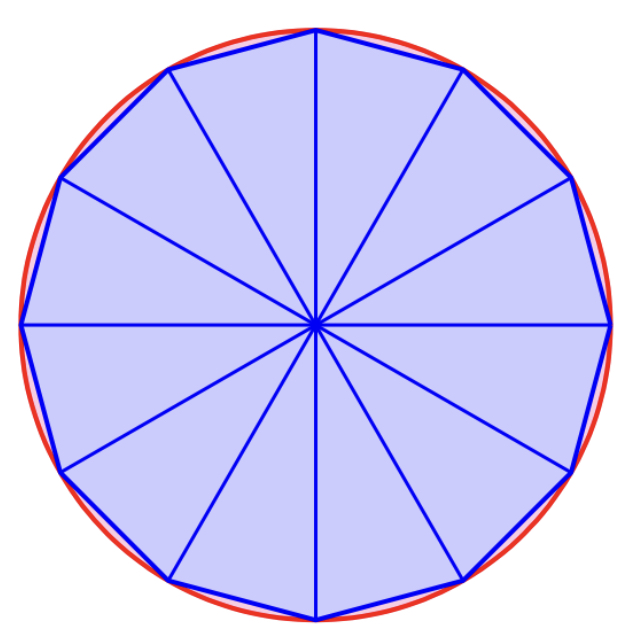
\includegraphics[scale=0.2]{Picture36.png}
\caption{ Approximating the area of a circle by the area of a polygon.\fa}\label{figure36}
\end{figure}

The same idea can be used to find the area enclosed by any curves. This motivated the definition of integrals. For curves defined by continuous functions, it is not difficult to formulate a well-defined definition for integrals. However, mathematicians soon discovered that we need to work with functions that are not continuous as well. The process to make integrals rigorously defined is long and tedious. We will follow the historical path and study the Riemann integrals in this course. This lays down the foundation for advanced theory of integration $\grave{\text{a}}$ la Lebesgue. For practical applications and computations, Riemann integrals are sufficient and easier to calculate.

\section{Riemann Integrals of Bounded Functions }\label{sec4.1}

In this section, we  define the Riemann integral for a function $f:[a,b]\to\mathbb{R}$ that is defined on a closed and bounded interval $[a,b]$. For this purpose, the function is necessarily bounded. In Section \ref{sec4.6}, we will discuss how to deal with functions that are not necessarily bounded, via some limiting processes. 

For  a closed and bounded interval $[a,b]$, we will always assume that $a<b$.
We start by a few definitions.
\begin{definition}{Partitions}
Let $[a, b]$ be a closed and bounded interval. A partition of $[a,b]$ is a finite sequence of points $x_0, x_1, x_2, \ldots, x_k$, where
\[a=x_0<x_1<\cdots<x_{k-1}<x_k=b.\]
 It is denoted by $P=\{x_0, x_1, \ldots, x_k\}$. For each $0\leq i\leq k$, $x_i$ is a partition point. These points partition the interval $[a, b]$ into $k$ subintervals $[x_0, x_1]$, $[x_1, x_2]$, $\ldots$, $[x_{k-1}, x_k]$. The $i^{\text{th}}$-subinterval is $[x_{i-1}, x_i]$.
\end{definition}We have slightly abused notation and used set notation for a partition.  
\begin{example}{}
$P=\{0, 2, 3, 5, 9, 10\}$ is a partition of the interval $[0,10]$ into 5 subintervals 
\[[0, 2], [2, 3], [3, 5], [5, 9]\;\text{and}\;[9,10].\]
\end{example}
We use the lengths of the subintervals to measure how fine a partition is. 
\begin{definition}{Gap of a Partition}
Let $P=\{x_0, x_1, \ldots, x_k\}$ be a partition of the interval $[a,b]$. The gap of the partition $P$, denoted by $|P|$ or $\text{gap}\,P$, is the length of the largest subinterval in the partition. Namely,
\[|P|=\text{gap}\, P=\max\left\{x_i-x_{i-1}\,|\, 1\leq i\leq k\right\}.\]
\end{definition}
\begin{example}{}For the partition $P=\{0, 2, 3, 5, 9, 10\}$ of $[0, 10]$,
\[|P|=\max\{2,1,2,4,1\}=4.\]
\end{example}
A partition where all subintervals have equal lengths is very useful.
\begin{definition}{Regular Partitions}
Let $[a, b]$ be a closed and bounded interval. A regular partition of $[a,b]$ into $k$ intervals is the partition 
$P=\{x_0, x_1, \ldots, x_k\}$, where 
\[|P|=x_1-x_0=x_2-x_1=\cdots=x_k-x_{k-1}=\frac{b-a}{k}.\]This implies that
$\di x_i=x_0+i\frac{b-a}{k}$, $1\leq i\leq k$.

\end{definition}
 \begin{example}{}
The  regular partition of the interval $[0,10]$ into 5 intervals is the partition 
\[P=\{0, 2, 4, 6, 8, 10\}.\]The gap of this partition is
$\di |P|=\frac{10-0}{5}=2$.
\end{example}

Next, we define the Riemann sums and Darboux sums.

\begin{definition}{Riemann Sums}
Let $f:[a,b]\to \mathbb{R}$ be a   function, and let $P=\{x_0, x_1, \ldots, x_k\}$ be a partition of $[a, b]$. For each $1\leq i\leq k$, choose an intermediate point $\xi_i$ in the $i^{\text{th}}$-subinterval $[x_{i-1}, x_i]$. Denote this sequence of points    $\{\xi_i\}_{i=1}^k$ by $A$. Then the Riemann sum of $f$ with respect to the partition $P$ and the intermediate points $A=\{\xi_i\}_{i=1}^k$ is the sum
\[R(f, P, A)=\sum_{i=1}^kf(\xi_i)(x_i-x_{i-1}).\]
\end{definition}

\begin{example}[label=ex230220_1]{}
Consider the function $f:[0, 6]\to\mathbb{R}$, $f(x)=6x-x^2$, and the partition  $P=\{0, 2, 3, 5, 6\}$ of $[0, 6]$. Let 
\[A=\left\{1, 3, 4, 5\right\}.\]Then 
\[R(f, P, A)=5\times 2+9\times 1+8\times 2+5\times   1=40.\]
\end{example}
As shown in Figure \ref{figure37}, the Riemann sum $R(f, P, A)$ is the sum of the areas of rectangles that are used to approximate the region bounded by the curve $y=6x-x^2$ and the $x$-axis. 

 \begin{figure}[ht]
\centering
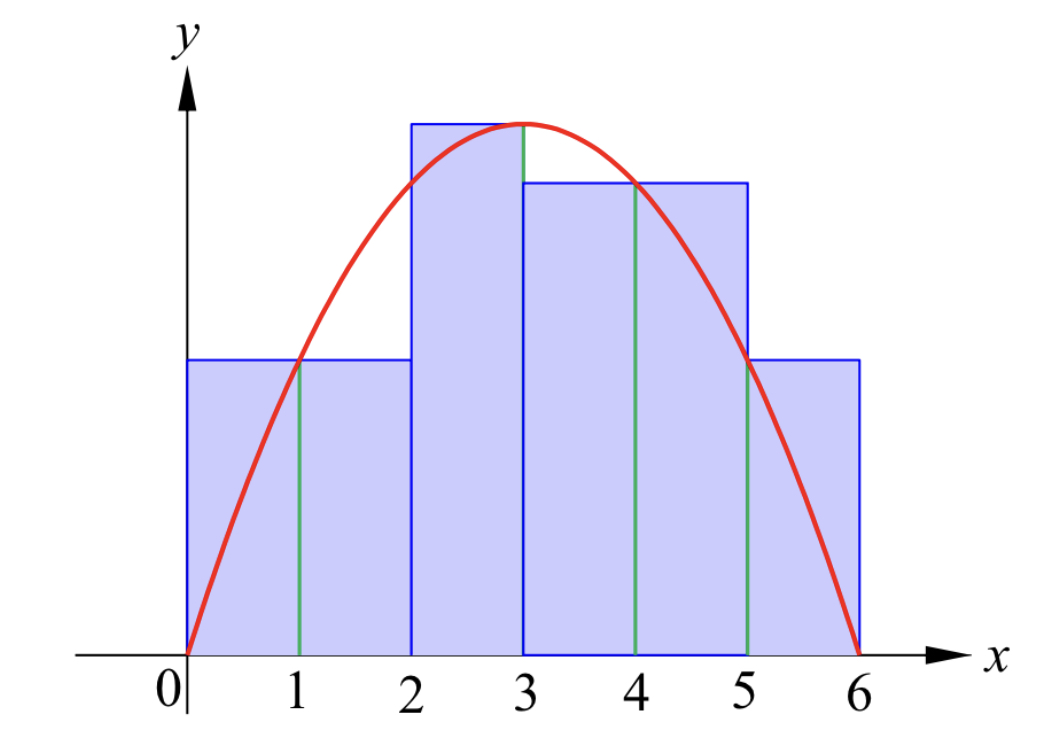
\includegraphics[scale=0.2]{Picture37.png}
\caption{Riemann sum is an approximation of area under a curve.\fa}\label{figure37}
\end{figure}

In general, if $f:[a,b]\to\mathbb{R}$ is a nonnegative function, then a Riemann sum $R(f, P, A)$ is an approximation to the area bounded by the curve $y=f(x)$, the $x$-axis, and the lines $x=a$ and $x=b$. In its definition, we do not need to assume that $f$ is a bounded function. 
Since Riemann sum involves an arbitrary choice of points in each subinterval, to give a bound to Riemann sums, we need the concept of Darboux sums, whose definition requires $f:[a,b]\to\mathbb{R}$ to be a bounded function.

\begin{definition}{Darboux Sums}
Let $f:[a,b]\to \mathbb{R}$ be a bounded function, and let $P=\{x_0, x_1, \ldots, x_k\}$ be a partition of $[a, b]$. For each $1\leq i\leq k$, let
\[m_i =\inf_{x_{i-1}\leq x\leq x_i}f(x),\hspace{1cm}
M_i =\sup_{x_{i-1}\leq x\leq x_i}f(x).\]The Darboux lower sum $L(f,P)$ and the Darboux upper sum $U(f,P)$ are defined by
\begin{align*}
L(f,P)&=\sum_{i=1}^km_i(x_i-x_{i-1}),\\
U(f,P)&=\sum_{i=1}^kM_i(x_i-x_{i-1}).
\end{align*}
\end{definition}
\begin{remark}{}
For convenience, we   denote \[ \inf \{f(x)\,|\,x_{i-1}\leq x\leq x_i\}\quad\text{and}\quad\sup\{f(x)\,|\,x_{i-1}\leq x\leq x_i\}\] by
$\di \inf_{x_{i-1}\leq x\leq x}f(x)$ and $\di \sup_{x_{i-1}\leq x\leq x_i}f(x)$ respectively. The assumption that $f$ is bounded is needed to ensure that $m_i$ and $M_i$ exist for all $1\leq i\leq k$. The reason we use infimum and supremum is obvious, as the function $f$ might not have minimum or maximum on an interval.
\end{remark}
 \begin{figure}[ht]
\centering
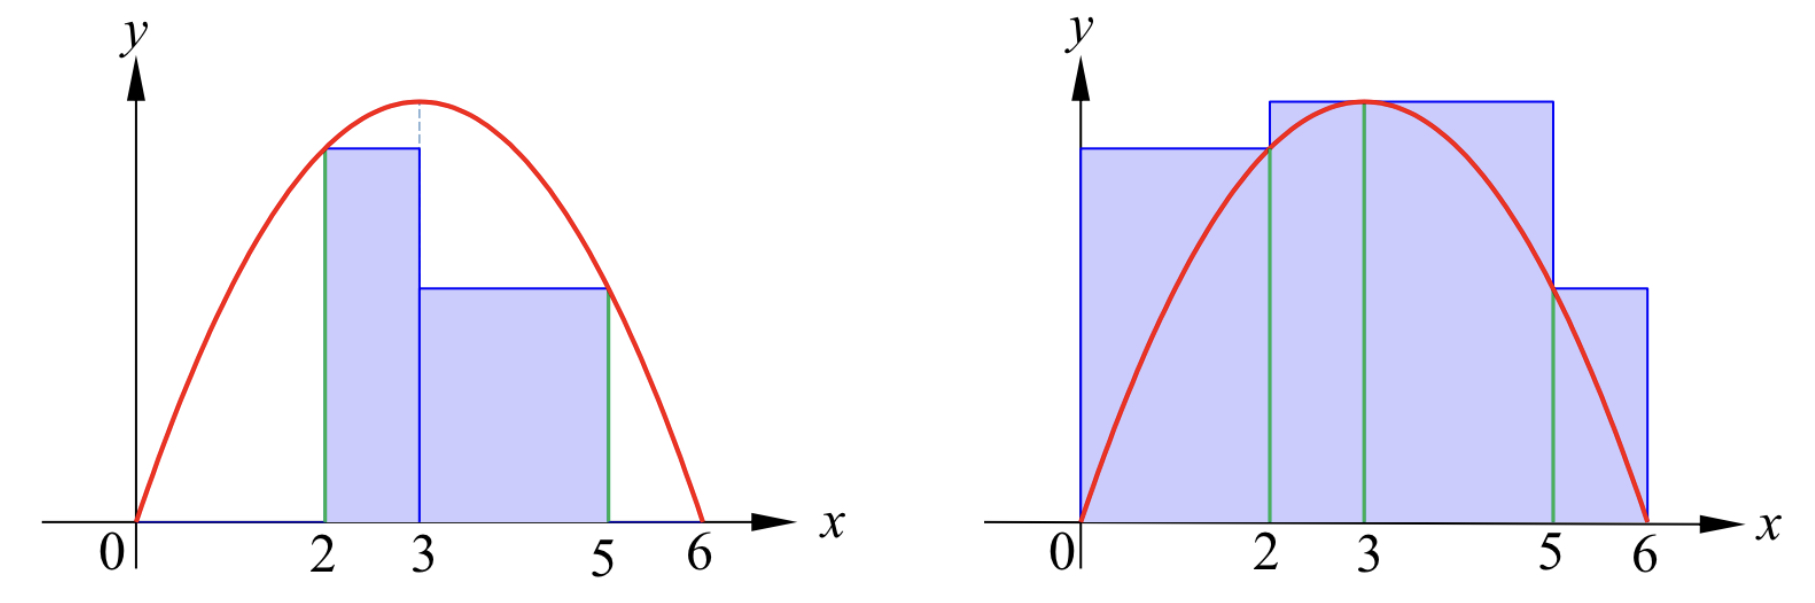
\includegraphics[scale=0.2]{Picture38.png}
\caption{Darboux lower sum and Darboux upper sum.\fa}\label{figure38}
\end{figure}
\begin{example}[label=ex230220_2]{}
For the   function $f:[0, 6]\to\mathbb{R}$, $f(x)=6x-x^2$  and the partition  $P=\{0, 2, 3, 5, 6\}$ of $[0, 6]$ considered in Example \ref{ex230220_1}, we find that

\vspace{0.5cm} ~\hspace{1.5cm}
\begin{tabular}{||c||c|c|c|c||}
\hline
\hline
$i$ &$\;$ interval$\;$ & $x_i-x_{i-1}$ & $m_i$ & $M_i$\\
\hline
\hline
$\;\;1\;\;$ & $[0,2]$ & 2&$\quad 0\quad $ & $\quad 8\quad $\\
\hline
2 & $[2,3]$ &1& 8 & 9\\
\hline
3 & $[3, 5]$ &2&  5&9\\
\hline 
4 & $[5, 6]$ &1& 0 & 5\\
\hline

\hline

\end{tabular}

\vspace{0.5cm}
Hence, the Darboux lower sum $L(f,P)$ and the Darboux upper sum $U(f,P)$ are
\begin{align*}
L(f,P)&=0\times 2+8\times 1+5\times 2+0\times   1=18,\\
U(f,P)&=8\times 2+9\times 1+9\times 2+5\times   1= 48.
\end{align*}
\end{example}
 


\begin{example}{}
If $f:[a,b]\to\mathbb{R}$ is the constant function $f(x)=c$, it is obvious that for any partition $P=\{x_i\}_{i=0}^k$ of $[a,b]$, and for any choices of intermediate points $A=\{\xi_i\}_{i=1}^k$,
\[L(f,P)=U(f,P)=R(f,P,A)=c(b-a).\]
\end{example}

The following can be easily deduced  from the definitions.
\begin{proposition}[label=230304_6]{}
Let $f:[a,b]\to\mathbb{R}$ be a bounded function such that
\[m\leq f(x)\leq M\hspace{1cm}\text{for all}\;a\leq x\leq b.\] For any partition $P=\{x_i\}_{i=0}^k$ of the interval $[a,b]$, and any  choice of intermediate points  $A=\{\xi_i\}_{i=1}^k$ for the partition $P$, we have
\[m(b-a)\leq L(f,P)\leq R(f,P,A)\leq U(f,P)\leq M(b-a).\]
\end{proposition}
\begin{myproof}{Proof}
For any $1\leq i\leq k$, let
\[m_i=\inf_{x_{i-1}\leq x\leq x}f(x),\hspace{1cm}
M_i =\sup_{x_{i-1}\leq x\leq x_i}f(x).\]Then 
\[m\leq m_i\leq f(\xi_i)\leq M_i\leq M.\] Therefore,
\begin{align*}
m(x_i-x_{i-1}) \leq m_i(x_i-x_{i-1})&\leq f(\xi_i)(x_i-x_{i-1})\\&\leq M_i(x_i-x_{i-1})\leq M(x_i-x_{i-1}).\end{align*}
Summing over $i$ from $i=1$ to $i=k$, we obtain
\[m(b-a)\leq L(f,P)\leq R(f,P,A)\leq U(f,P)\leq M(b-a).\]
\end{myproof}

For a  bounded nonnegative   function $f:[a,b]\to \mathbb{R}$,  if the region bounded by the $x$-axis, the curve $y=f(x)$, the lines $x=a$ and $x=b$ has an area, then a Darboux lower sum  is always less than or  equal to the area, and a Darboux upper sum   is always larger than or equal to the area. This leads to the fact that a Darboux lower sum is always less than or equal to a Darboux upper sum. To prove this for any bounded functions, we introduce the concept of refinement.

\begin{definition}{Refinement of a Partition}
Let $P$ and $P^*$ be partitions of the interval $[a,b]$. We say that $P^*$ is refinement of $P$ if every partition point of $P$ is also a partition point of $P^*$. In other words, the set of points in $P$ is a subset of the set of points in $P^*$.
\end{definition}

 \begin{example}[label=ex230220_3]{}
For the partition $P=\{0, 2, 3, 5, 9, 10\}$ of $[0,10]$, \[P^*=\{0, 1, 2, 3, 5, 6, 8, 9, 10\}\] is a refinement.
\end{example}
 \begin{figure}[ht]
\centering
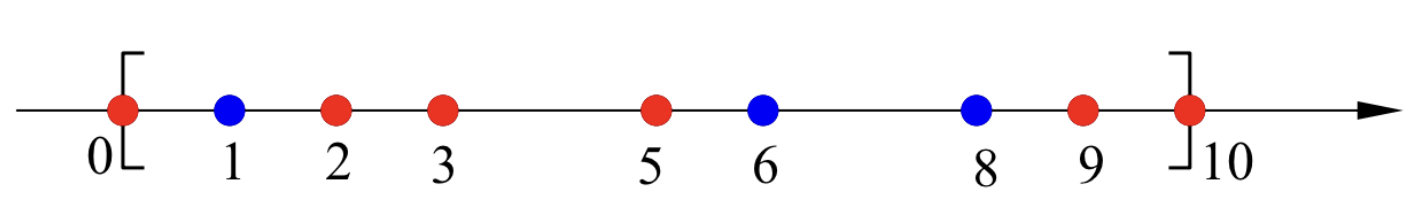
\includegraphics[scale=0.2]{Picture39.png}
\caption{A partition $P$ of $[0,10]$ and its refinement $P^*$.\fa}\label{figure39}
\end{figure}

If $P^*$ is a refinement of $P=\{x_i\}_{i=1}^k$, then for each $1\leq i\leq k$, $P^*$ induces a partition $P_i$ of the interval $[x_{i-1}, x_i]$. 

 \begin{example}[label=ex230220_4]{}
For the partition $P$ and $P^*$ in Example \ref{ex230220_3}, $P^*$ induces the partition $P_1=\{0,1,2\}$, $P_2=\{2,3\}$, $P_3=\{3,5\}$, $P_4=\{5,6,8,9\}$ and $P_5=\{9,10\}$ of the intervals $[0,2]$, $[2,3]$,  $[3,5]$, $[5,9]$ and $[9,10]$ respectively. 
\end{example}

Since the union of all the subintervals in the partition $P_i$, $1\leq i\leq k$ is the collection of all the subintervals in the partition $P^*$, the following is quite obvious.
\begin{proposition}[label=230220_5]{}
Let $f:[a,b]\to\mathbb{R}$ be a bounded function, and let $P=\{x_i\}_{i=0}^k$ be a partition of $[a,b]$. Given a refinement $P^*$ of $P$,  let $P_i$, $1\leq i\leq k$, be the partition that $P^*$ induces on the interval $[x_{i-1}, x_i]$. Then
\[\sum_{i=1}^kL(f,P_i)=L(f,P^*),\hspace{1.5cm} \sum_{i=1}^kU(f,P_i)=U(f,P^*).\]
\end{proposition}

From this, it is quite easy to obtain the following. 
\begin{theorem}[label=230220_6]{}
Let $f:[a,b]\to\mathbb{R}$ be a bounded function, and let $P$ and $P^*$ be   partitions of $[a,b]$. If $P^*$ is a refinement of $P$, then
\[L(f,P)\leq L(f,P^*)\leq U(f,P^*)\leq U(f,P).\]

\end{theorem}
\begin{myproof}{Proof}Let $P=\{x_i\}_{i=0}^k$. For each $1\leq i\leq k$, 
let
\[m_i=\inf_{x_{i-1}\leq x\leq x_i}f(x),\hspace{1cm}M_i=\sup_{x_{i-1}\leq x\leq x_i}f(x).\]
Since 
\[m_i\leq f(x)\leq M_i\hspace{1cm}\text{for all}\;x\in [x_{i-1}, x_i],\]
we find that
\[m_i(x_i-x_{i-1})\leq L(f, P_i)\leq U(f,P_i)\leq M_i(x_i-x_{i-1}).\]Summing over $i$ from $1$ to $k$ gives
\[\sum_{i=1}^{k}m_i(x_i-x_{i-1})\leq\sum_{i=1}^{k} L(f, P_i)\leq \sum_{i=1}^{k}U(f,P_i)\leq \sum_{i=1}^{k}M_i(x_i-x_{i-1}).\]By Proposition \ref{230220_5}, this gives
\[L(f,P)\leq L(f,P^*)\leq U(f,P^*)\leq U(f,P).\]
\end{myproof}

\begin{figure}[ht]
\centering
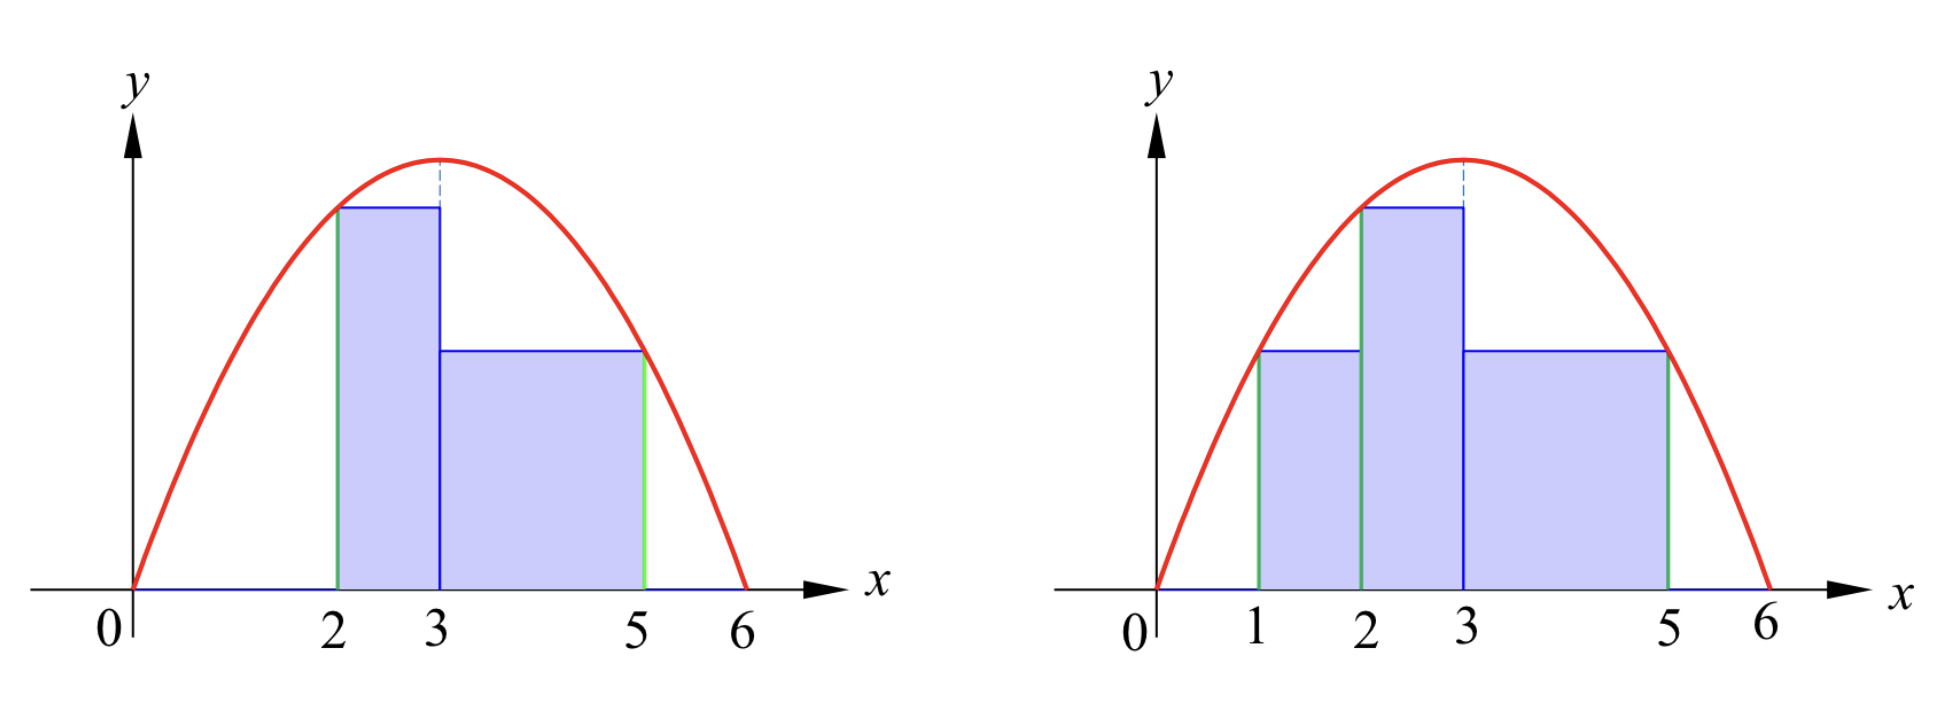
\includegraphics[scale=0.2]{Picture40.png}
\caption{When a partition is refined, Darboux lower sum gets larger.\fa}\label{figure40}
\end{figure}

\begin{figure}[ht]
\centering
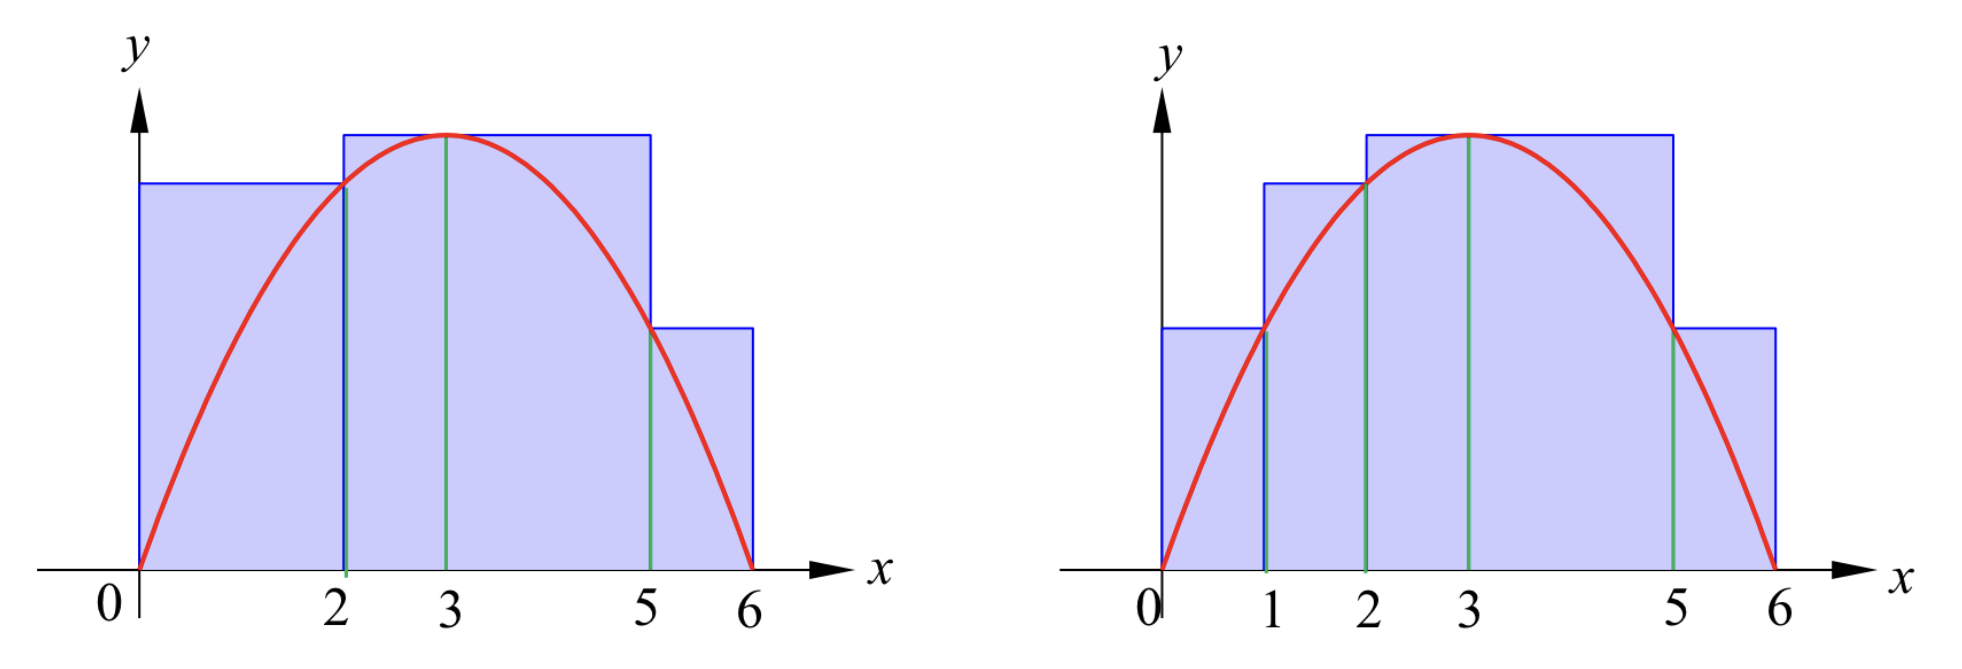
\includegraphics[scale=0.2]{Picture41.png}
\caption{When a partition is refined, Darboux upper sum gets smaller.\fa}\label{figure41}
\end{figure}

If $P_1$ and $P_2$ are partitions of $[a,b]$, a common refinement of $P_1$ and $P_2$ is a partition $P^*$ which contains all the partition points of $P_1$ and $P_2$. Such a common refinement always exists. The smallest one is the one whose set of points is the union of the set of points in $P_1$ and the set of points in $P_2$.
\begin{corollary}[label=230220_7]{}
Let $f:[a,b]\to\mathbb{R}$ be a bounded function, and let $P$ and $P_2$ be any  two partitions of $[a,b]$. Then
\[L(f, P_1)\leq U(f, P_2).\]
\end{corollary}
\begin{myproof}{Proof}
Take a common refinement $P^*$ of the partitions $P_1$ and $P_2$. By Theorem \ref{230220_6},
\[L(f,P_1)\leq L(f,P^*)\leq U(f,P^*)\leq U(f,P_2).\]
\end{myproof}

Given a bounded function $f:[a,b]\to\mathbb{R}$, we consider the set of Darboux lower sums and the set of Darboux upper sums of $f$.
\begin{align*}
S_L(f)&=\left\{L(f,P)\,|\, P\;\text{is a partition of}\;[a,b]\right\},\\
S_U(f)&=\left\{U(f,P)\,|\, P\;\text{is a partition of}\;[a,b]\right\}.
\end{align*}If $m$ and $M$ are lower and upper bounds of $f$, then 
\[m(b-a)\leq L(f,P)\leq U(f,P)\leq M(b-a).\]
This implies that the sets $S_L(f)$ and $S_U(f)$ are bounded. When we use the Darboux lower sums and upper sums to approximate areas, we are interested in the least upper bound of the lower sums and the greatest lower bound of the upper sums.
\begin{definition}{Lower Integrals and Upper Integrals}
Let $f:[a,b]\to\mathbb{R}$ be a bounded function.
\begin{enumerate}[1.]
\item
The lower integral of $f$, denoted by $\di\underline{\int_a^b}f$, is defined as the least upper bound of the Darboux lower sums.
\[\underline{\int_a^b}f=\sup S_L(f)=\sup \left\{L(f,P)\,|\, P\;\text{is a partition of}\;[a,b]\right\}.\]
\item
The upper integral of $f$, denoted by $\di\overline{\int_a^b}f$, is defined as the greatest lower bound of the Darboux upper sums.
\[\overline{\int_a^b}f=\inf S_U(f)=\inf \left\{U(f,P)\,|\, P\;\text{is a partition of}\;[a,b]\right\}.\]
\end{enumerate}
\end{definition}

\begin{example}{}
For the constant function $f:[a.,b]\to\mathbb{R}$, $f(x)=c$, 
\[L(f,P)=U(f,P)=c(b-a)\] for any partition $P$ of $[a,b]$. Thus,
$S_L(f)=S_U(f)=\{c(b-a)\}$, and
\[\underline{\int_a^b}f=\overline{\int_a^b}f=c(b-a).\]
\end{example}

By Corollary \ref{230220_7}, we have the following.
\begin{proposition}{}
Let $f:[a,b]\to\mathbb{R}$ be a bounded function. We have
\[\underline{\int_a^b}f\leq \overline{\int_a^b}f.\]
\end{proposition}
\begin{myproof}{Proof}
By definitions of infimum and supremum, for any positive integer $n$, there are partition $P_1$ and $P_2$ such that
\[L(f,P_1)>\underline{\int_a^b}f-\frac{1}{n},\hspace{1cm}U(f,P_2)< \overline{\int_a^b}f+\frac{1}{n}.\]
These, together with Corollary \ref{230220_7}, give the following.
\[ \overline{\int_a^b}f-\underline{\int_a^b}f>U(f,P_2)-L(f,P_1)-\frac{2}{n}\geq -\frac{2}{n}.\]
Taking the limit $n\to\infty$, we deduce that
\[\overline{\int_a^b}f-\underline{\int_a^b}f\geq 0.\]
\end{myproof}
\begin{highlight}{}
Let $f:[a,b]\to\mathbb{R}$ be a bounded function, and let  $P$ be a partition of $[a,b]$.
\begin{enumerate}[1.]
\item $\di L(f,P)\;\leq \;\underline{\int_a^b} f\;\leq \;\overline{\int_a^b }f \;\leq U(f,P)$.
\item $\di 0\;\leq \;\overline{\int_a^b }f \;-\;\underline{\int_a^b} f\;\leq\;U(f,P)\;-\;L(f,P)$.

\end{enumerate}
\end{highlight}
Notice that if $w$ is a number such that
\[\underline{\int_a^b}f\leq w\leq \overline{\int_a^b}f,\]then
for any partition $P$ of $[a,b]$,
\[L(f,P)\leq w\leq U(f,P).\]
As we mentioned above, for a nonnegative bounded function $f:[a,b]\to\mathbb{R}$, a Darboux lower sum $L(f,P)$ is less  than or equal to the area below the curve $y=f(x)$, while a Darboux upper sum is larger than or equal to the area, if such an area is well-defined. Intuitively, the area would be well-defined if there is a single number $A$ that is larger than or equal to all the Darboux lower sums, and less than or equal to all the Darboux upper sums. This is the case if and only if the lower and the upper integrals are the same. 
\begin{definition}{Riemann Integrability}
Let $f:[a,b]\to \mathbb{R}$ be a bounded function. We say that $f$ is Riemann integrable, or simply integrable, if 
\[\underline{\int_a^b}f= \overline{\int_a^b}f.\]In this case, we define the integral of $f$ over $[a,b]$ as
\[\int_a^b f=\underline{\int_a^b}f=\overline{\int_a^b}f.\]
It is the unique number  that is larger than or equal to all the Darboux lower sums, and less than or equal to all the Darboux upper sums.
\end{definition}

\begin{remark}{}
If $f:[a,b]\to \mathbb{R}$ is a continuous nonnegative function, we are going to prove that $f$ is Riemann integrable.  It follows from our discussions above that 
the integrable $\di\int_a^b f$ is the area bounded by the curve $y=f(x)$, the $x$-axis, and the lines $x=a$ and $x=b$.
\end{remark}

\begin{highlight}{Leibniz Notation}
In Leibniz notation, the integral of $f:[a,b]\to\mathbb{R}$ over $[a,b]$ is denoted by \[\int_a^b f(x)dx.\]
\end{highlight}
\begin{example}{}
A constant functon $f:[a,b]\to\mathbb{R}$, $f(x)=c$  is integrable and 
\[\int_a^b f =c(b-a).\]
\end{example}

Let us look at an example of a function that is not integrable.
 \begin{example}[label=230220_9]
 {Non-Integrability of the Dirichlet's Function} The Dirichlet's function is the function $f:[0,1]\rightarrow\mathbb{R}$ defined by
 \begin{align*}
 f(x)=\begin{cases}1,\quad &\text{if}\; x\;\text{is rational},
 \\0,\quad &\text{if}\; x\;\text{is irrational}.\end{cases}
 \end{align*}
Show that $f$ is not Riemann integrable.
 \end{example}
\begin{solution}{Solution}
Let $P=\{x_i\}_{i=0}^k$ be any partition of the interval $[0,1]$. For any $1\leq i\leq k$, by denseness of the set of rational numbers and the set of irrational numbers, there exist a rational number and an irrational number in the interval $[x_{i-1}, x_i]$.  This shows that \[m_i=0,\hspace{1cm}M_i=1,\hspace{1cm}\text{for all}\;1\leq i\leq k.\]
Hence, 
\begin{align*}L(f,P)&=\sum_{i=1}^k m_i(x_i-x_{i-1})=0,\\ U(f,P)&=\sum_{i=1}^k M_i(x_i-x_{i-1})=1.\end{align*}
This shows that  
\[S_L(f)=\{0\},\hspace{1cm}S_U(f)=\{1\}.\]
Therefore, the lower integral and the upper integral of $f$ are
\[\underline{\int_a^b}f=0,\hspace{1cm}\overline{\int_a^b}f=1\]respectively. Since they are not equal, $f$ is not Riemann integrable.
\end{solution}

An interesting question now is what functions are Riemann integrable. 
Let us first give alternative criteria for Riemann integrability.
\begin{lemma}[label=230220_10]
{}
Let $f:[a,b]\to\mathbb{R}$ be a bounded function. Then the following are equivalent.
\begin{enumerate}[(a)]
\item $f:[a,b]\to\mathbb{R}$  is Riemann integrable.
\item For any $\varepsilon>0$, there exists a partition $P$ of $[a,b]$ such that
\[U(f,P)-L(f,P)<\varepsilon.\]
 

\end{enumerate}
\end{lemma}
\begin{myproof}{Proof}
First, let us prove (a)  implies  (b). If $f$ is Riemann integrable, \[\int_a^bf=\underline{\int_a^b}f =\overline{\int_a^b} f.\] Given $\varepsilon>0$, by definitions of lower and upper integrals as supremums and infimums, there exist partitions $P_1$ and $P_2$ of $[a,b]$ such that
\[L(f,P_1)>\int_a^b f-\frac{\varepsilon}{2}\hspace{1cm}\text{and}\hspace{1cm}
U(f,P_2)<\int_a^b f+\frac{\varepsilon}{2}.\]
This gives 
\[U(f,P_2)-L(f,P_1)<\varepsilon.\]
Let $P$ be a common refinement of $P_1$ and $P_2$. Then
\[L(f,P_1)\leq L(f,P)\leq U(f,P)\leq U(f,P_2).\]
This implies that
\[
U(f,P)-L(f,P) \leq U(f,P_2)-L(f,P_1)< \varepsilon.
\]
Conversely, assume that (b) holds. Then for every positive integer $n$, there is a partition $P_n$ of $[a,b]$ such that\bp
\[0\leq \;U(f,P_n)\;-\;L(f,P_n)<\frac{1}{n}.\]
Therefore,
\[0\leq\overline{\int_a^b }f \;-\;\underline{\int_a^b} f <\frac{1}{n}.\]
Taking the  $n\to \infty$ limit, squeeze theorem implies that
\[\underline{\int_a^b} f\;=\;\overline{\int_a^b }f.\]
This shows that $f$ is Riemann integrable.
\end{myproof}
 
\begin{theorem}[label=230220_11]
{The Archimedes-Riemann Theorem}
Let $f:[a,b]\to\mathbb{R}$ be a bounded function. Then $f:[a,b]\to\mathbb{R}$  is Riemann integrable if and only if there is a sequence $\{P_n\}$ of partitions of $[a,b]$ such that
\begin{equation}\label{eq230220_12}\lim_{n\to \infty}(U(f,P_n)-L(f,P_n))=0.\end{equation}
In this case, the Riemann integral of $f$ over $[a,b]$ can be computed by
\begin{equation}\label{eq230220_13}\int_a^b f=\lim_{n\to\infty}L(f,P_n)=\lim_{n\to\infty}U(f,P_n).\end{equation}
\end{theorem}

This theorems says that the Riemann integrability of a function can be checked by the existence of a sequence of partitions satisfying \eqref{eq230220_12}. Such sequence of partitions can also be used to compute the   Riemann integral. Thus, we give such sequence a special name.
\begin{definition}{Archimedes Sequence of Partitions}
Let $f:[a,b]\to\mathbb{R}$ be a bounded function. A sequence $\{P_n\}$ of partitions of $[a,b]$ is called an Archimedes sequence of partitions for $f$ provided that
\[\lim_{n\to \infty}(U(f,P_n)-L(f,P_n))=0.\]
\end{definition}Hence, Theorem \ref{230220_11} says that $f:[a,b]\to\mathbb{R}$ is Riemann integrable if and only if it has an Archimedes sequence of partitions. 

\begin{myproof}{\linkt Proof of Theorem \ref{230220_11}}
If $f:[a,b]\to\mathbb{R}$ is Riemann integrable,  by Lemma \ref{230220_10}, for every positive integer $n$, there is a partition $P_n$ of $[a,b]$ such that
\[0\leq U(f,P_n)-L(f,P_n)<\frac{1}{n}.\]
 By squeeze theorem,
\[\lim_{n\to\infty}(U(f,P_n)-L(f,P_n))=0.\] Conversely, if there is a sequence $\{P_n\}$ of partitions of $[a,b]$ such that
\[\lim_{n\to \infty}(U(f,P_n)-L(f,P_n))=0,\]  the definition of limit of sequences implies that for every $\varepsilon>0$, there is a positive integer $N$ such that for all $n\geq N$,
\[|U(f,P_n)-L(f,P_n)|<\varepsilon.\]In particular, we find that $P_N$ is a partition of $[a,b]$ satisfying
\[U(f,P_N)-L(f,P_N)<\varepsilon.\]
By Lemma \ref{230220_10} again, we find that $f$ is Riemann integrable.
This means $\di\int_a^bf=\underline{\int_a^b}f =\overline{\int_a^b} f$. Therefore,
\[0\;\leq\; U(f,P_n)\;-\;\int_a^b f\;\leq U(f,P_n)-L(f,P_n).\]
By taking the $n\to \infty$ limit, we find that
\[\lim_{n\to \infty}U(f,P_n)=\int_a^bf.\]Since $\di \lim_{n\to \infty}(U(f,P_n)-L(f,P_n))=0$, we find that
  \[\lim_{n\to \infty}L(f,P_n)=\lim_{n\to \infty}U(f,P_n)=\int_a^bf.\]  
\end{myproof}

Let us look at an example how to apply the Archimedes-Riemann theorem to compute integrals.
\begin{example}[label=ex230221_4]{}
Let $f:[1, 4]\to\mathbb{R}$ be the function $f(x)=x^2 $. Show that $f$ is Riemann integrable and find the integral $\di \int_1^4f(x)dx$.
\end{example}
Here we need the formulas
\[\sum_{i=1}^ni=\frac{n(n+1)}{2},\hspace{1cm}\sum_{i=1}^ni^2=\frac{n(n+1)(2n+1)}{6}.\]
\begin{solution}{Solution}
 Let $n$ be a positive integer, and let $P_n=\{x_0, x_1, \ldots, x_n\}$ be the regular partition of $[1,4]$ into $n$  intervals. Then
\[x_i=1+\frac{3i}{n}.\]
Notice that  the function $f:[1, 4]\to\mathbb{R}$, $f(x)=x^2 $ is an increasing function. Therefore, on the interval $[x_{i-1}, x_i]$, 
\[m_i=f(x_{i-1})=\left(1+\frac{3i-3}{n}\right)^2,\hspace{1cm}M_i=f(x_i)=\left(1+\frac{3i}{n}\right)^2.\]
From this, we find that
\begin{align*}
L(f,P_n)&=\sum_{i=1}^nm_i(x_i-x_{i-1})=\frac{3}{n}\sum_{i=1}^n\left(1+\frac{6(i-1)}{n}+\frac{9(i-1)^2}{n^2}\right)\\
&=\frac{3}{n}\left(n+3(n-1)+\frac{3(n-1)(2n-1)}{2n}\right)\\
&=\frac{3}{2n^2}(14n^2-15n+3),
\end{align*}\bs
\begin{align*}
U(f,P_n)&=\sum_{i=1}^nM_i(x_i-x_{i-1})=\frac{3}{n}\sum_{i=1}^n\left(1+\frac{6i}{n}+\frac{9i^2}{n^2}\right)\\
&=\frac{3}{n}\left(n+3(n+1)+\frac{3(n+1)(2n+1)}{2n}\right)\\
&=\frac{3}{2n^2}(14n^2+15n+3).
\end{align*}Moreover,
\[U(f,P_n)-L(f,P_n)=\frac{45}{n}.\]
It follows that
\[\lim_{n\to\infty}\left(U(f,P_n)-L(f,P_n)\right)=0.\]This proves that $\{P_n\}$ is an Archimedes sequence of partitions for $f$. Therefore, $f$ is Riemann integrable, and
\[\int_1^4f(x)dx=\lim_{n\to\infty}U(f,P_n)=\lim_{n\to\infty} \frac{3}{2 }\left(14 +\frac{15}{n}+\frac{3}{n^2}\right)=21.\]
\end{solution}

The following gives an $\varepsilon-\delta$ characterization of Riemann integrability   in terms of Darboux sums.
\begin{theorem}[label=230221_2]{Equivalent Definitions of Riemann Integrability}
Let  $f:[a,b]\to\mathbb{R}$ be a bounded function. Then the following two statements are equivalent.
\begin{enumerate}[(i)]
\item $f:[a,b]\to\mathbb{R}$ is Riemann integrable, in the sense that $\di \underline{\int_a^b }f=\overline{\int_a^b} f$.
\item 
For any $\varepsilon>0$, there exists a $\delta>0$ so that   if $P=\{x_i\}_{i=0}^{k}$ is a partition of $[a,b]$ with $|P|<\delta$,  then
\[U(f,P)-L(f,P)<\varepsilon.\]
\end{enumerate}
 
 
\end{theorem}
 By Lemma  \ref{230220_10}, $f:[a,b]\to\mathbb{R}$ is Riemann integrable if and only if for every $\varepsilon>0$, there is a partition $P$ satisfying $U(f,P)-L(f,P)<\varepsilon$. The highly nontriviality of this theorem is   the existence of a single partition satisfying $U(f,P)-L(f,P)<\varepsilon$ is equivalent to the existence of a positive number $\delta$ such that \emph{all} partitions $P$ with gaps less than $\delta$   satisfy $U(f,P)-L(f,P)<\varepsilon$.

\begin{myproof}{Proof}
 (ii) implies (i) follows trivially from  Lemma  \ref{230220_10}.

  

Now assume that (i) holds.
Since $f:[a,b]\to\mathbb{R}$ is bounded, there exists a positive number $M$ such that
\[|f(x)|\leq M\hspace{1cm}\text{for all}\;x\in [a,b].\]
Given $\varepsilon>0$,  Lemma \ref{230220_10} implies that  there is a partition \[P_0=\{\widetilde{x}_0, \widetilde{x}_1, \ldots, \widetilde{x}_s\}\] of $[a,b]$ such that
\[U(f,P_0)-L(f,P_0)<\frac{\varepsilon}{2}.\]
Take
\[\delta=\frac{\varepsilon}{8sM}.\] Then $\delta>0$. If $P=\{x_0, x_1, \ldots, x_k\}$ is a partition of $[a,b]$ with $|P|<\delta$, we want to show that
\[U(f, P)-L(f,P)=\sum_{i=1}^k(M_i-m_i)(x_i-x_{i-1})<\varepsilon.\]
Here\[m_i=\inf_{x_{i-1}\leq x\leq x_i}f(x),\hspace{1cm}M_i=\sup_{x_{i-1}\leq x\leq x_i}f(x).\]   
 Let
\[E_1=\left\{1\leq i\leq k\,|\, \exists j,\;\widetilde{x}_j\in [x_{i-1}, x_i]\right\}\]
be the set that contains those indices $i$ where the interval $[x_{i-1}, x_i]$ contains a partition point of $P_0$, and
let $E_2=\{1, 2, \ldots, k\}\setminus E_1$ be the set of those indices that are not in $E_1$. 
\bp
  By definition, the point $\widetilde{x}_0$ can only be in $[x_0, x_1]$, and the point $\widetilde{x}_s$ can only be in $[x_{k-1}, x_k]$. For any $1\leq j\leq s-1$, $\widetilde{x}_j$ can be in at most two different subintervals of $P$. Hence, $E_1 $ contains at most $2s$ elements.
 
 

Splitting the sum over $i$ to a sum over $E_1$ and a sum over $E_2$, we have
\[U(f,P)-L(f,P)=\sum_{i\in E_1}(M_i-m_i)(x_i-x_{i-1})+\sum_{i\in E_2}(M_i-m_i)(x_i-x_{i-1}).\] 
First we estimate the sum over $E_1$. 
 Since \[-M\leq f(x)\leq M\quad\text{ for all }\;x\in [a,b],\] we find that for any $1\leq i\leq k$,
\[0\leq M_i-m_i\leq 2M.\]
Since $x_i-x_{i-1}\leq|P|<\delta$, we have 
\[\sum_{i\in E_1}(M_i-m_i)(x_i-x_{i-1})\leq \sum_{i\in E_1}2M(x_i-x_{i-1})\leq 2M\delta |E_1|\leq 4sM\delta \leq\frac{\varepsilon}{2}.\]Let $P^*$ be the common refinement of $P$ and $P_0$ obtained by taking the union of their partition points. By our definitions of $E_1$ and $E_2$, for each $i$ in $E_2$, $[x_{i-1}, x_i]$ is also a partition interval in $P^*$. 
 Therefore,
\begin{align*} \sum_{i\in E_2}\left(M_i-m_i\right)(x_i-x_{i-1}) &\leq U(f,P^*)-L(f,P^*)\\&\leq U(f,P_0)-L(f,P_0)<\frac{\varepsilon}{2}.\end{align*}
 The two estimates above imply that
\[U(f,P)-L(f,P)<  \varepsilon,\]
which completes the proof that (i)  implies (ii).
\end{myproof}


A disadvantage of working with Darboux sums is we need to figure out the infimum and supremum of a function over the partition intervals. Let us turn to Riemann sums.

\begin{lemma}[label=230221_3]{}
Let $f:[a,b]\to\mathbb{R}$ be a bounded function, and let $P=\{x_i\}_{i=0}^k$ be a partition of $[a,b]$.
 For every  $\varepsilon>0$, there exist   choices of intermediate points $A$ and  $B$ for the partition $P$ such that
\begin{align*}
0\leq R(f,P,A)-L(f,P)<\varepsilon,\quad
 0\leq U(f, P)- R(f,P,B) <\varepsilon.\end{align*}
 
\end{lemma}
\begin{myproof}{Proof}For $1\leq i\leq k$, let
$\di m_i=\inf_{x_{i-1}\leq x\leq x_i}f(x)$ and $\di M_i=\sup_{x_{i-1}\leq x\leq x_i}f(x)$.
By definitions of infimum and supremum, for each $1\leq i\leq k$, there are points $\xi_i$ and $\eta_i$ in $[x_{i-1}, x_i]$ such that
\begin{gather*}
m_i\leq f(\xi_i)<m_i+\frac{\varepsilon}{ (b-a)},\\  M_i-\frac{\varepsilon}{ (b-a)}<f(\eta_i)\leq M_i.\end{gather*}
Multiply  by $(x_i-x_{i-1})$ and sum  over $i$, we find that
\begin{equation*} \begin{split}
\sum_{i=1}^km_i(x_i-x_{i-1})\leq \sum_{i=1}^kf(\xi_i)(x_i-x_{i-1}) <\sum_{i=1}^km_i(x_i-x_{i-1})+ \varepsilon,\\
\sum_{i=1}^kM_i(x_i-x_{i-1})- \varepsilon<\sum_{i=1}^kf(\eta_i)(x_i-x_{i-1})\leq  \sum_{i=1}^kM_i(x_i-x_{i-1}).
\end{split}\end{equation*}
Let $A=\{\xi_i\}_{i=1}^k$ and  $B=\{\eta_i\}_{i=1}^k$. They are choices of intermediate points for the partition $P$.  The two inequalities above give
\begin{gather*}
L(f,P)\leq R(f,P,A)<L(f,P)+\varepsilon,\\ U(f,P)-\varepsilon<R(f,P,B)\leq U(f,P),\end{gather*}which are the desired results.
\end{myproof}

The following gives an $\varepsilon-\delta$ definition for Riemann integrability of a bounded function.
\begin{theorem}[label=230220_15]{Equivalent Definitions of Riemann Integrability}
Let $f:[a,b]\to\mathbb{R}$ be a bounded function. Consider  the following two definitions for $f$ to be Riemann integrable.
\begin{enumerate}[(i)]
\item $\di \underline{\int_a^b }f=\overline{\int_a^b} f$.

\item There is a number $I$ such that for any $\varepsilon>0$, there exists a $\delta>0$ so that   if $P=\{x_i\}_{i=0}^{k}$ is a partition of $[a,b]$ with $|P|<\delta$, $A=\{\xi_i\}_{i=1}^k$ is a choice of intermediate points for $P$, then
\[|R(f,P,A)-I|<\varepsilon.\]

\end{enumerate}
These two statements are equivalent, and in case $f$ is Riemann integrable, \[I=\underline{\int_a^b }f=\overline{\int_a^b} f=\int_a^b f.\]
\end{theorem}
Note that statement  (ii) can be  expressed as saying the limit of Riemann sums
\[I=\lim_{|P| \to 0}R(f, P, A)\]exists.
 

\begin{myproof}{Proof}
 
Assume that (i) holds. 
Let \[I=\underline{\int_a^b }f=\overline{\int_a^b} f.\]
Given $\varepsilon>0$, by Theorem \ref{230221_2}, there exists a $\delta>0$ such that if $P=\{x_i\}_{i=0}^k$ is a partition of $[a,b]$ with $|P|<\delta$, then 
\[U(f,P)-L(f,P)<\varepsilon.\]\bp
If $A=\{\xi_i\}_{i=1}^k$ is any choice of intermediate points for the partition $P$,  
\[L(f,P)\leq R(f, P, A)\leq U(f,P).\] Since we also have
\[L(f,P)\leq I\leq U(f,P),\]we find that
\[|R(f, P, A)-I|\leq  U(f,P)-L(f,P)<\varepsilon.\]
This proves that (i) implies (ii).



Conversely,   assume that (ii) holds. By Lemma \ref{230220_10}, to show that (i) holds, it suffices to prove that
  for any $\varepsilon>0$, there is a partition $P$ of $[a,b]$ so that
\[U(f,P)-L(f,P)<\varepsilon.\]
Given $\varepsilon>0$, (ii) implies   there is  a $\delta>0$ such that if $P=\{x_i\}_{i=0}^{k}$ is a partition of $[a,b]$ with $|P|<\delta$, $A=\{\xi_i\}_{i=1}^k$ is a choice of intermediate points for the partition $P$, then
\begin{equation}\label{eq230220_16}|R(f,P,A)-I|<\frac{\varepsilon}{4}.\end{equation}Here $I$ is the limit of Riemann sums implied by (ii).  Let $P=\{x_i\}_{i=0}^n$ be  a regular partition into $n$ intervals, where $n$ is large enough so that \[|P|=\frac{b-a}{n} <\delta.\] By Lemma \ref{230221_3}, there exist choices of intermediate points $A$ and $B$ for the partition $P$ which satisfy
\[U(f,P)<R(f,P,A)+\frac{\varepsilon}{4},\hspace{1cm} L(f,P)>R(f,P,B)-\frac{\varepsilon}{4}.\] 
These imply that
\[U(f,P)-L(f,P)<R(f,P,A)-R(f,P,B)+\frac{\varepsilon}{2}.\]
 \bp By \eqref{eq230220_16},
\[|R(f,P,A)-R(f,P,B)|\leq |R(f,P,A)-I|+|R(f,P,B)-I|<\frac{\varepsilon}{2}.\]
This proves that
\[U(f,P)-L(f,P)<\varepsilon,\]which completes the proof that  (ii)  implies  (i). 

 
\end{myproof}
As a consequence of Theorem \ref{230221_2} and Theorem \ref{230220_15}, we have the following.
\begin{corollary}[label=230618_1]{}
Let $f:[a,b]\to\mathbb{R}$ be a bounded function that is Riemann integrable, and let $\{P_n\}$ be a sequence of partitions of $[a,b]$ such that
\[\lim_{n\to \infty}|P_n|=0.\]Then 
 \begin{enumerate}[(a)]
\item
$\di \int_a^b f=\lim_{n\to \infty}U(f,P_n)= \lim_{n\to \infty}L(f,P_n)$
\item $\di \int_a^b f=\lim_{n\to \infty}R(f,P_n, A_n)$, where for each $n\in\mathbb{Z}^+$, $A_n$ is a choice of intermediate points for the partition $P_n$.
\end{enumerate}
\end{corollary}
This corollary says that if we \emph{ know apriori } that $f:[a,b]\to\mathbb{R}$ is Riemann integrable, then we can evaluate the integral by a sequence of partitions whose gaps goes to 0, using either the Darboux upper sums, or the Darboux lower sums, or Riemann sums for any choice of intermediate points.  



\begin{myproof}{Proof}
Let $I=\di\int_a^bf$. Given $\varepsilon>0$, Theorem \ref{230221_2} and Theorem \ref{230220_15} imply that there is a $\delta>$ such that for any partition $P$ with $|P|<\delta$, and any choice of intermdiates points $A$ for the partition $P$,  
\[U(f,P)-L(f,P)<\varepsilon \hspace{1cm}\text{and}\hspace{1cm}|R(f, P, A)-I|<\varepsilon.\]\bp
Since $\di\lim_{n\to \infty}|P_n|=0$, there is a positive integer $N$ so that for all $n\geq N$, $|P_n|<\delta$. This implies that
for all $n\geq N$, 
\[U(f,P_n)-L(f,P_n)<\varepsilon \quad\text{and}\quad|R(f, P_n, A_n)-I|<\varepsilon.\]
Since $L(f,P_n)\leq I\leq U(f,P_n)$,
we find that
\[|U(f,P_n)-I|<\varepsilon\quad\text{and}\quad|L(f,P_n)-I|<\varepsilon \quad\text{for all}\;n\geq N.\]
These prove that
\[I=\lim_{n\to \infty}U(f,P_n) =\lim_{n\to \infty}L(f,P_n)=\lim_{n\to \infty}R(f,P_n, A_n).\]
\end{myproof}
\begin{highlight}{}For every positive integer $n$, take $P_n$ to be the regular partition of $[a,b]$ into $n$ intervals.  This gives a sequence of partitions $\{P_n\}$ with \[\lim_{n\to \infty}|P_n|=\lim_{n\to\infty}\frac{b-a}{n}=0.\] For the choices of intermediate points $A_n$, one can take the left end point of each interval, or the right end point, or the midpoint. \end{highlight}
\begin{example}{}
We are going to prove in Section \ref{sec4.3} that a continuous function is integrable. The function $f:[0, 6]\to\mathbb{R}$, $f(x)=6x-x^2 $ is continuous. Use Riemann sums to evaluate the integral $\di \int_0^6f(x)dx$.
\end{example}
\begin{solution}{Solution}
For a positive integer $n$, let $P_n=\{x_i\}_{i=0}^n$ be the regular partition of $[0,6]$ into $n$ intervals. Then
\[x_i=\frac{6i}{n},\hspace{1cm} 0\leq i\leq n.\]\bs
Let $A_n=\{\xi_i\}_{i=1}^n$, where
\[\xi_i=x_i=\frac{6i}{n}, \quad 1\leq i\leq n.\]  Then
\begin{align*}
R(f,P_n,A_n)&=\sum_{i=1}^nf(\xi_i)(x_i-x_{i-1})\\&=\frac{6}{n}\sum_{i=1}^n\left(\frac{36i}{n}-\frac{36i^2}{n^2}\right)\\
&=\frac{216}{n^2}\left(\frac{n (n+1)}{2}-\frac{ (n+1)(2n+1)}{6}\right)\\
&=\frac{36(n^2-1)}{n^2}.
\end{align*}
Therefore,
\[\int_0^6f(x)dx=\lim_{n\to\infty}R(f,P_n,A_n)=36.\]
\end{solution}
\vp
\noindent
{\bf \large Exercises  \thesection}
\setcounter{myquestion}{1}


\begin{question}{\themyquestion}
Let $f:[0, 2]\to\mathbb{R}$ be the function $f(x)=4-x^2 $. Given a positive integer $n$, let $P_n$ be the regular partition of $[0,2]$ into $n$ subintervals.
\begin{enumerate}[(a)]
\item Compute $L(f,P_n)$ and $U(f, P_n)$.
\item Show directly that $\di \lim_{n\to\infty}\left(U(f,P_n)-L(f,P_n)\right)=0$.
\item Use part (b) to conclude that $f$ is Riemann integrable and find the integral $\di \int_0^2f(x)dx$.
\end{enumerate}
\end{question}
 \atc



\begin{question}{\themyquestion}Given that the functon $f:[0, 4]\to\mathbb{R}$, $f(x)=x^2-2x+3$ is Riemann integrable. Use Riemann sums to evaluate the integral $\di \int_0^4f(x)dx$.
\end{question}
\vp

\section{Properties of Riemann Integrals  }\label{sec4.2}
In this section, we derive some properties of the Riemann integrals.
First we show that integral of a nonnegative function is nonnegative.
\begin{theorem}[label=230221_5]{}
If $f:[a,b]\to\mathbb{R}$ is a bounded function that is Riemann integrable, and \[f(x)\geq 0\hspace{1cm} \text{for all}\;x\in [a, b],\] then \[\int_a^b f\geq 0.\]
\end{theorem}
\begin{myproof}{Proof}
Since $f$ is Riemann integrable,  
\[\int_a^b f=\lim_{n\to \infty}L(f,P_n),\]
where $P_n$ is the regular partition of $[a,b]$ into $n$ intervals. 
Since $f(x)\geq 0$ for all $x\in [a, b]$, we find that\[L(f,P_n)\geq 0\hspace{1cm}\text{for all }\;n\in\mathbb{Z}^+.\] Therefore,
\[\int_a^b f\geq 0.\]
\end{myproof}

Linearity is always an important property. 
\begin{theorem}[label=230221_6]{Linearity of Integrals}
Let $f:[a,b]\to\mathbb{R}$ and $g:[a,b]\to\mathbb{R}$ be bounded functions. If $f$ and $g$ are Riemann integrable, then for any constants $\alpha$ and $\beta$, $\alpha f+\beta g:[a,b]\to\mathbb{R}$ is also Riemann integrable, and
\[\int_a^b(\alpha f+\beta g)=\alpha\int_a^b f+\beta \int_a^b g.\]
\end{theorem}
\begin{myproof}{Proof}
Here we   use   the fact that a function $h:[a,b]\to\mathbb{R}$ is Riemann integrable if and only if the limit
$\di \lim_{|P|\to 0}R(h,P,A)$ exists.  Since  $f:[a,b]\to\mathbb{R}$ and $g:[a,b]\to\mathbb{R}$ are bounded, $\alpha f+\beta g$ is also bounded. Since  $f:[a,b]\to\mathbb{R}$ and $g:[a,b]\to\mathbb{R}$ are Riemann integrable, 
\[\int_a^b f=\lim_{|P|\to 0}R(f,P,A),\hspace{1cm}\int_a^bg=\lim_{|P|\to 0}R(g,P,A).\]
Notice that for any partition $P=\{x_i\}_{i=0}^k$ of $[a,b]$, and any choice of intermediate points $A=\{\xi_i\}_{i=1}^k$ for the partition $P$,
\begin{align*}R(\alpha f+\beta g, P, A)&=\sum_{i=1}^k\left(\alpha f(\xi_i)+\beta g(\xi_i)\right)(x_i-x_{i-1})\\
&=\alpha R(f,P,A)+\beta R(g,P,A).\end{align*}
Limit laws imply that
\begin{align*}\lim_{|P|\to 0}R(\alpha f+\beta g, P, A)&=\alpha\lim_{|P|\to 0}R(f,P,A)+\beta\lim_{|P|\to 0}R(g,P,A)\\&=\alpha \int_a^b f+\beta\int_a^b g.\end{align*}
This proves that $\alpha f+\beta g $ is  Riemann integrable and
\[\int_a^b(\alpha f+\beta g)=\alpha\int_a^b f+\beta \int_a^b g.\]
\end{myproof}

From the previous two theorems, we   obtain a comparison theorem for integrals.
\begin{theorem}{Monotonicity}
Let $f:[a,b]\to\mathbb{R}$ and $g:[a,b]\to\mathbb{R}$ be bounded functions. If $f$ and $g$ are Riemann integrable, and 
\[f(x)\geq g(x)\hspace{1cm}\text{for all}\;x\in [a,b],\]
then
\[\int_a^b f\geq \int_a^b g.\]
\end{theorem}
\begin{myproof}{Proof}
Define $h:[a,b]\to\mathbb{R}$ to be the function
$h(x)=f(x)-g(x)$.
Then 
$h(x)\geq 0$ for all $x\in [a,b]$. 
By Theorem \ref{230221_6}, $h$ is Riemann integrable and 
\[\int_a^b h=\int_a^b f-\int_a^b g.\]
By Theorem \ref{230221_5}, $\di\int_a^b h\geq 0$. Hence,
\[\int_a^b f\geq \int_a^b g.\]
\end{myproof}
We can apply the monotonicity theorem to obtain  bounds for  an integral  from the lower bound and the upper bound of the function.
\begin{example}{}
Let $f:[a,b]\to\mathbb{R}$ be a Riemann integrable funtion satisfying 
\[m\leq f(x)\leq M\hspace{1cm}\text{for all}\;x\in [a,b].\]
Then
\[m(b-a)\;\leq\;\int_a^b f\;\leq\; M(b-a).\]
\end{example}

When an interval is partitioned into a finite collection of intervals,
the integral over the whole interval is expected to equal to the sum of the intergrals over the subintervals. It is enough for us to consider two subintervals.
\begin{theorem}{Additivity}
Let $f:[a,b]\to\mathbb{R}$ be a bounded function, and let $c$ be a point in $(a,b)$.
\begin{enumerate}[(a)]
\item
If $f:[a,b]\to\mathbb{R}$ is Riemann integrable, then  $f:[a,c]\to\mathbb{R}$  and $f:[c,b]\to\mathbb{R}$  are Riemann integrable.
\item If $f:[a,c]\to\mathbb{R}$  and $f:[c,b]\to\mathbb{R}$  are Riemann integrable, then $f:[a,b]\to\mathbb{R}$ is Riemann integrable. 
\end{enumerate}In either case,
\[\int_a^b f=\int_a^c f+\int_c^b f.\]
\end{theorem}

\begin{myproof}{Proof}
We use  Lemma \ref{230220_10}.  First we prove (a). Given $\varepsilon>0$, since $f:[a,b]\to\mathbb{R}$ is Riemann integrable, there is a partition $P$ of $[a,b]$ such that
\[U(f,P)-L(f,P)<\varepsilon.\]
Let $P^*$ be the partition of $[a,b]$ that is obtained  by taking the union of the partition points in $P$ and $P_0=\{a, c, b\}$. If $P$ already contains $c$ as a partition point, then $P^*=P$. In any case, $P^*$ is a refinement of $P$.   Therefore,
\[U(f,P^*)-L(f,P^*)\leq U(f,P)-L(f,P)<\varepsilon.\]
Consider $P^*$ as a refinement of $P_0$, let $P_1$ be the partition of $[a,c]$   induced by $P^*$, and let $P_2$ be the partition of $[c, b]$ induced by $P^*$. Then
\[L(f,P^*)=L(f,P_1)+L(f,P_2), \hspace{1cm}U(f,P^*)=U(f,P_1)+U(f,P_2).\]
These imply that
\[(U(f,P_1)-L(f,P_1))+(U(f,P_2)-L(f,P_2))=U(f,P^*)-L(f,P^*)<\varepsilon.\]
\bp Since $U(f,P_1)-L(f,P_1)\geq 0$ and $U(f,P_2)-L(f,P_2)\geq 0$, we find that
\[U(f,P_1)-L(f,P_1)<\varepsilon\quad\text{and}\quad U(f,P_2)-L(f,P_2)<\varepsilon.\]
By Lemma \ref{230220_10},  we conclude that $f:[a,c]\to\mathbb{R}$  and $f:[c,b]\to\mathbb{R}$  are Riemann integrable.
 
Next, we prove (b). Given $\varepsilon>0$,  since $f:[a,c]\to\mathbb{R}$  and $f:[c,b]\to\mathbb{R}$  are Riemann integrable, there exists a partition $P_1$ of $[a,c]$, and a partition $P_2$ of $[c,b]$ such that 
\[U(f,P_1)-L(f,P_1)<\frac{\varepsilon}{2}\quad\text{and}\quad U(f,P_2)-L(f,P_2)<\frac{\varepsilon}{2}.\]
Let $P$ be the partition of $[a,b]$ obtained by taking the union of the partition points in $P_1$ and $P_2$. Then 
\[L(f,P )=L(f,P_1)+L(f,P_2), \hspace{1cm}U(f,P )=U(f,P_1)+U(f,P_2).\]Therefore,
\[U(f,P)-L(f,P)=(U(f,P_1)-L(f,P_1))+(U(f,P_2)-L(f,P_2))<\varepsilon.\]
This proves that $f:[a,b]\to\mathbb{R}$ is Riemann integrable.

Now we prove the last statement.
For any positive integer $n$,   let $P_{1,n}$ be the regular partition of $[a,c]$ into $n$ intervals, and let $P_{2,n}$ be the regular partition of $[c,b]$ into $n$ intervals. Then let $P_n$ be the partition of $[a,b]$ obtained by taking the union of the partition points in $P_{1,n}$ and $P_{2,n}$.  For the Darboux upper sums, we have 
\[U(f,P_n)=U(f,P_{1,n})+U(f,P_{2,n}).\] 
Taking the $n\to \infty$ limits on both sides, we conclude that
\[\int_a^b f=\int_a^c f+\int_c^b f.\]
\end{myproof}
\begin{highlight}{Extension of Definition of Integrals}
The additivity allows us to extend the definition of the integral $\di \int_a^b f$ to the case where $a\geq b$. We define
\[\int_a^a f=0.\] If $a>b$, define
\[\int_a^b f=-\int_b^a f.\]
Then one can check that 
as long as two of the three  integrals $\di\int_a^b f$, $\di \int_a^cf$, $\di \int_c^bf$ exist, the third one also exists, and we always have
\[\int_a^b f=\int_a^c f+\int_c^b f.\]

\end{highlight}

Using induction, we can extend the additivity theorem.
\begin{corollary}[label=230221_9]{General Additivity Theorem}
Let $f:[a,b]\to\mathbb{R}$ be a bounded function, and let $P_0=\{a_0, a_1, \ldots, a_k\}$ be a partition of $[a,b]$. Then $f:[a,b]\to\mathbb{R}$ is Riemann integrable if and only if for each $1\leq i\leq k$, $f:[a_{i-1},a_i]\to\mathbb{R}$ is Riemann integrable. In this case,
\[\int_a^b f(x)dx=\int_{a}^{a_1}f+\int_{a_1}^{a_2}f+\cdots+\int_{a_{k-2}}^{a_{k-1}}f+\int_{a_{k-1}}^bf.\]
\end{corollary}
\vp
\noindent
{\bf \large Exercises  \thesection}
\setcounter{myquestion}{1}

\begin{question}{\themyquestion}
Given that $f:[2, 7]\to\mathbb{R}$ is a function satisfying
\[-3\leq f(x)\leq 11\hspace{1cm} \text{for all}\;x\in [2, 7].\]
Find a lower bound and an upper bound for $\di \int_2^7f(x)dx$. 
\end{question}

\atc
\begin{question}{\themyquestion}
Given that $f:[a,b]\to\mathbb{R}$ and $g:[a,b]\to\mathbb{R}$ are bounded functions,  $P$ is a partition of $[a,b]$, and $c$ and $d$ are two points in $[a, b]$ with $c<d$. Prove the following.
\begin{enumerate}[(a)]
\item $\di\inf_{c\leq x\leq d}(f+g)(x)\geq \inf_{c\leq x\leq d}f(x)+\inf_{c\leq x\leq d}g(x)$.
\item  $\di\sup_{c\leq x\leq d}(f+g)(x)\leq \sup_{c\leq x\leq d}f(x)+\sup_{c\leq x\leq d}g(x)$.
\item $L(f+g, P)\geq L(f, P)+L(g, P)$.
\item $U(f+g,P)\leq U(f,P)+U(g,P)$.
\end{enumerate}
  Then use (c) and (d) to give a proof of the following statement: If  $f:[a,b]\to\mathbb{R}$ and $g:[a,b]\to\mathbb{R}$ are Riemann integrable, then $f+g:[a,b]\to\mathbb{R}$ is also Riemann integrable, and
\[\int_a^b(f+g)=\int_a^b f+\int_a^b g.\]
\end{question}

 

 
\vp

\section{Functions that are Riemann Integrable}\label{sec4.3}
In this section, we are going to derive Riemann integrability of a few classes of functions. The first class of functions that are of interest is the class of continuous  functions. If $f:[a,b]\to\mathbb{R}$ is a continuous function, then $f([a,b])$ is sequentially compact. In particular, $f([a,b])$ is bounded. Hence, if $f:[a,b]\to\mathbb{R}$ is a continuous function, it is bounded. 
The crucial property for a continuous function defined on a closed and bounded interval to be integrable is   uniform continuity.  

\begin{theorem}[label=230221_7]{}
Let $f:[a,b]\to\mathbb{R}$ be a continuous function. Then $f:[a,b]\to\mathbb{R}$ is Riemann integrable.
\end{theorem}
\begin{myproof}{Proof}
Since  $f:[a,b]\to\mathbb{R}$ is a continuous function defined on a closed and bounded interval, it is uniformly continuous. Given $\varepsilon>0$, there exists $\delta>0$ such that for any $u$ and $v$ in $[a,b]$ with $|u-v|<\delta$,
\[|f(u)-f(v)|< \frac{\varepsilon}{b-a}.\]
Let $P=\{x_i\}_{i=0}^k$ be a partition of $[a,b]$ with $|P|<\delta$. For any $1\leq i\leq k$, $f:[x_{i-1},x_i]\to\mathbb{R}$ is continuous. By extreme value theorem, there exists $u_i$ and $v_i$ in $[x_{i-1}, x_i]$ such that
\[m_i=\inf_{x_{i-1}\leq x\leq x_i}f(x)=f(u_i),\hspace{1cm}M_i=\sup_{x_{i-1}\leq x\leq x_i}f(x)=f(v_i).\]Then
\[|u_i-v_i|\leq x_i-x_{i-1}\leq |P|<\delta.\]
Therefore,
\[M_i-m_i=f(v_i)-f(u_i)< \frac{\varepsilon}{b-a}.\]\bp
Hence,
\begin{align*}
U(f,P)-L(f,P)&=\sum_{i=1}^k (M_i-m_i)(x_i-x_{i-1}) \\&<\frac{\varepsilon}{b-a}\sum_{i=1}^k(x_i-x_{i-1}) =\varepsilon.\end{align*}
This proves that $f:[a,b]\to\mathbb{R}$ is Riemann integrable.
\end{myproof}

\begin{highlight}{}
It follows from this theorem that all the following classes of functions are integrable on a  closed and bounded interval that is contained in their domains.
\begin{enumerate}[$\bullet$\;\;]
\item Polynomials
\item Rational Functions
\item Exponential Functions
\item Logarithmic Functions
\item Trigonometric Functions

\end{enumerate}
\end{highlight} 

\begin{figure}[ht]
\centering
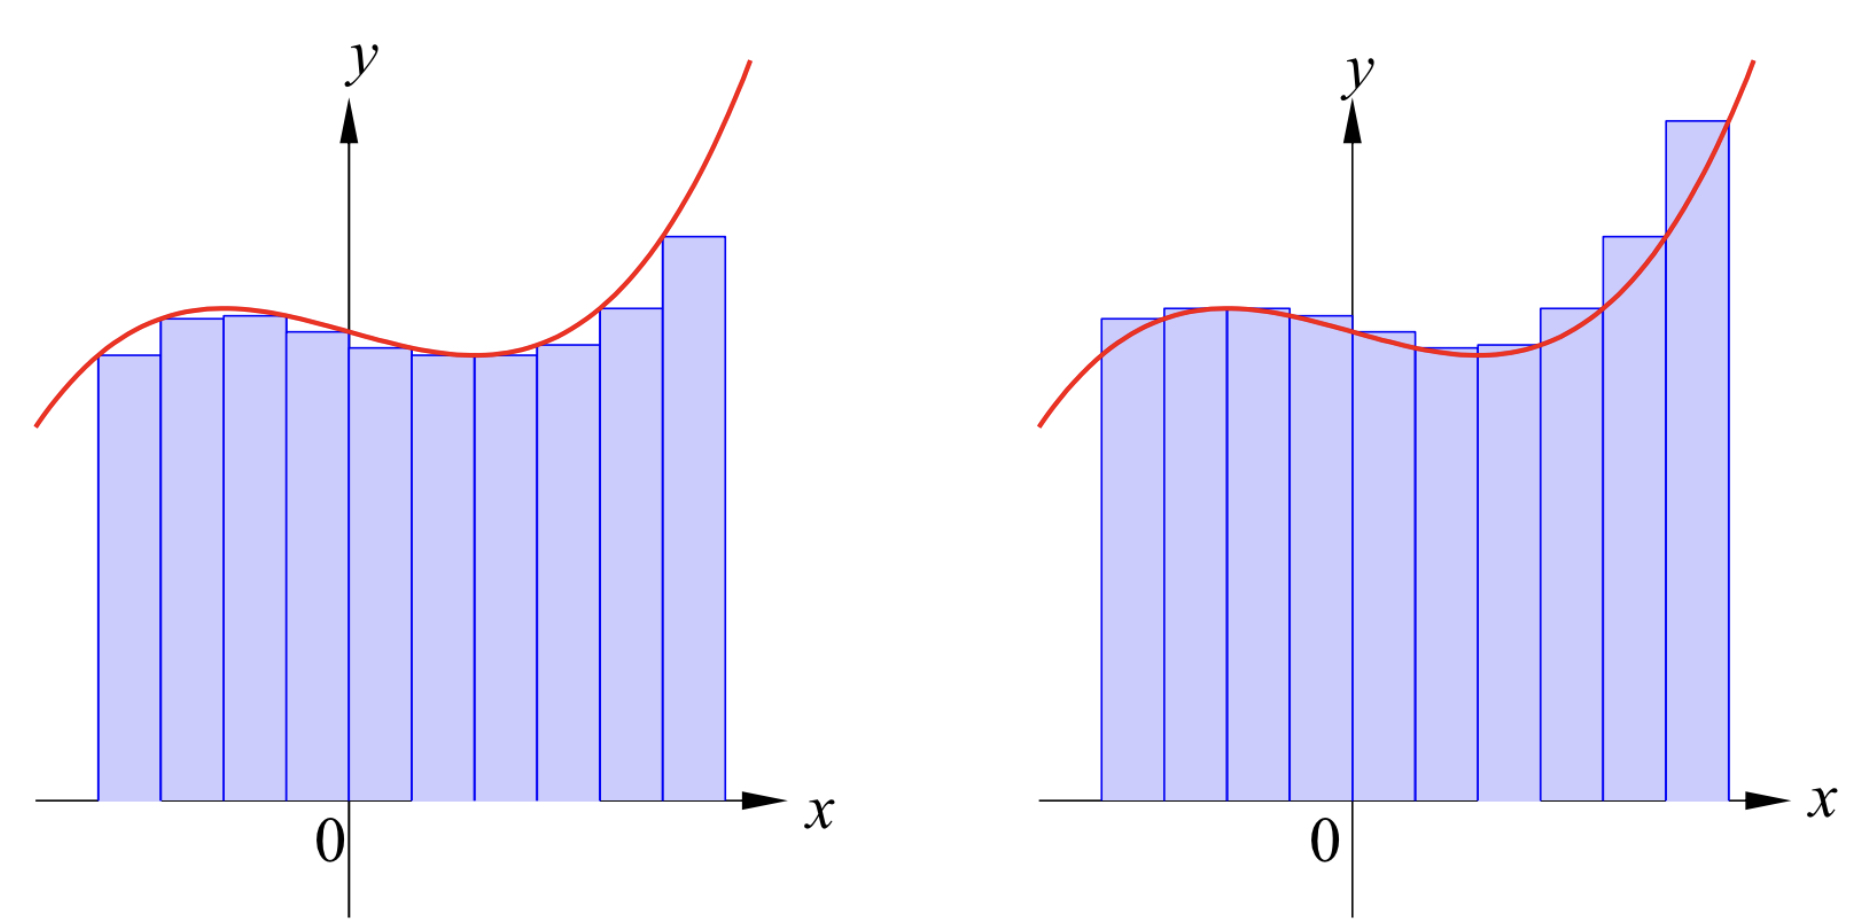
\includegraphics[scale=0.2]{Picture70.png}
\caption{Darboux lower sum underestimates area while Darboux upper sum overestimates area.  }\label{figure70}
\end{figure}
Let us revisit the concept of area, which is our original motivation to define integrals.
\begin{remark}{Area}
Let $f:[a,b]\to \mathbb{R}$ be a continuous function such that $f(x)\geq 0$ for all $x\in [a,b]$, and let $R$ be the region bounded between the $x$-axis, the lines $x=a$ and $x=b$, as well as the curve $y=f(x)$. 
\end{remark}\begin{highlight}{}Given $P$ a partition of $[a,b]$, the Darboux lower sum $L(f,P)$ is a sum of areas of rectangles that are inside $R$. The Darboux upper sum $U(f,P)$ is a sum of areas of rectangles whose union contains $R$. Therefore, if $R$ has a area $A$, $L(f,P)$ is less than or equal to  $A$, while $U(f,P)$ is larger than or equal to $A$. Since $f$ is continuous, the Riemann integral $\di I=\int_a^b f(x)dx$ exists. By definition, $I$ is the unique number such that
\[L(f,P)\leq I\leq U(f,P)\] for all partitions $P$ of $[a,b]$. Therefore, we define the area of $R$ to be this number $I$. Namely,
\[\text{Area of}\, R=\int_a^b f(x)dx.\]\end{highlight}

 




There are also other classes of functions that are Riemann integrable, which are useful. First, we relax the continuity condition slightly in the previous theorem.

\begin{theorem}[label=230221_8]{}
Let $f:[a,b]\to\mathbb{R}$ be a bounded  function that is continuous on $(a, b)$. Then $f:[a,b]\to\mathbb{R}$ is Riemann integrable.
\end{theorem}
Here we only assume $f$ is continuous on $(a,b)$. The function can take on any values on the boundary points $a$ and $b$.
\begin{myproof}{Proof}
Since  $f:[a,b]\to\mathbb{R}$ is bounded, there is a positive constant $M$ such that
\[|f(x)|\leq M\hspace{1cm}\text{for all}\;x\in [a,b].\]
Given $\varepsilon>0$, let 
\[r=\min\left\{\frac{\varepsilon}{8M}, \frac{b-a}{3}\right\}.\]Then $r>0$ and $a+r<b-r$. The function $f:[a+r, b-r]\to\mathbb{R}$ is continuous.  By Theorem \ref{230221_7}, $f:[a+r, b-r]\to\mathbb{R}$ is Riemann integrable.

 Therefore, there is a partition $P_1$ of $[a+r, b-r]$ such that
\[U(f,P_1)-L(f,P_1)<\frac{\varepsilon}{2}.\]
Let $P$ be the partition of $[a,b]$ obtained by adding the points $a$ and $b$ to $P_1$.  Then
\begin{align*}U(f,P)-L(f,P)&=U(f,P_1)-L(f,P_1)\\&\quad +r\left(\sup_{a\leq x\leq a+r}f(x)-\inf_{a\leq x\leq a+r}f(x)\right)\\&\quad +r\left(\sup_{b-r\leq x\leq b}f(x)-\inf_{b-r\leq x\leq b}f(x)\right)\\
&<\frac{\varepsilon}{2}+4Mr\\
&\leq \frac{\varepsilon}{2}+\frac{\varepsilon}{2}=\varepsilon.\end{align*}
This proves that $f:[a,b]\to\mathbb{R}$ is Riemann integrable.

\end{myproof}

As we can see in the proof above, the integral $\di\int_a^b f$ does not depend on the function value at the end points. In fact, this is true for  any finite number of points.
\begin{theorem}[label=230222_2]{}
Let $f:[a,b]\to\mathbb{R}$  be a bounded function that is Riemann integrable. Assume that $g:[a,b]\to\mathbb{R}$ is a function  and $S=\{ a_1, a_2, \ldots, a_k\}$ is a finite subset of $[a,b]$ such that
\[g(x)=f(x)\hspace{1cm}\text{for all}\; x\in [a,b]\setminus S.\]
Then  $g:[a,b]\to\mathbb{R}$ is Riemann integrable, and
\[\int_a^b g=\int_a^b f.\]
\end{theorem}

\begin{myproof}{Proof}
 

Let $h:[a,b]\to\mathbb{R}$ be the function $h(x)=g(x)-f(x)$. Then   $h(x)=0$ for $x\in  [a,b]\setminus S$. Since $S$ is a finite set, $h$ is bounded, and so there is a positive constant $M$ such that $|h(x)|\leq M$ for all $x\in [a,b]$. Given a positive integer $n$, let $P_n=\{x_0, x_1, \ldots, x_n\}$  be the regular partition of $[a,b]$ into $n$ intervals. There are at most $2k$ of the intervals $[x_{i-1}, x_i]$ that contains a point of $S$. In these intervals, 
\[-M\leq \inf_{x_{i-1}\leq x\leq x_i}h(x)\leq \sup_{x_{i-1}\leq x\leq x_i}h(x)\leq  M.\] If $[x_{i-1},x_i]$   does not contain any points of $S$, then 
\[\inf_{x_{i-1}\leq x\leq x_i}h(x)=\sup_{x_{i-1}\leq x\leq x_i}h(x)=0.\]
These imply that
\[U(h,P_n) =\sum_{i=1}^n \sup_{x_{i-1}\leq x\leq x_i}h(x) (x_{i}-x_{i-1})\leq  \frac{2Mk(b-a)}{n}.\]
\[L(h,P_n) =\sum_{i=1}^n \inf_{x_{i-1}\leq x\leq x_i}h(x) (x_{i}-x_{i-1})\geq   -\frac{2Mk(b-a)}{n}.\]
\bp
Therefore,
\[-\frac{2Mk(b-a)}{n}\leq L(h,P_n)\leq U(h,P_n)\leq \frac{2Mk(b-a)}{n}.\]
Taking $n\to \infty$ limits, we find that
\[\lim_{n\to\infty}  U(h,P_n)=\lim_{n\to\infty}L(h,P_n) =0.\]By the Archimedes-Riemann theorem, $h:[a,b]\to\mathbb{R}$
 is Riemann integrable and
$\di  \int_a^b h=0$.
Therefore, $g=h+f$ is also Riemann integrable and 
\[\int_a^b g=\int_a^bh+\int_a^bf=\int_a^b f.\]
\end{myproof}


\begin{remark}{}
If $f:(a,b)\to\mathbb{R}$ is a bounded function, we can extend the function to $[a,b]$ and discuss its integrability. By Theorem \ref{230222_2}, this is not affected by how we define the function at $x=a$ and $x=b$. In case the extension is Riemann integrable, we still denote the integral by $\di\int_a^b f$.
\end{remark}
\begin{definition}{Piecewise Continuous Functions}
We say that a function $f:[a,b]\to\mathbb{R}$ is piecewise continuous if there is a partition $P_0=\{a_0, a_1, \ldots, a_k\}$ of $[a,b]$ such that for each $1\leq i\leq k$, $f:(a_{i-1}, a_i)\to \mathbb{R}$ is continuous. 
\end{definition} 

Using the general additivity theorem (Corollary \ref{230221_9}) and Theorem \ref{230221_8}, we obtain the following immediately.
\begin{theorem}[label=230221_10]{}
Let $f:[a,b]\to\mathbb{R}$ be a function that is bounded and piecewise continuous. Then $f:[a,b]\to\mathbb{R}$ is Riemann integrable.
\end{theorem}

\begin{example}[label=ex230221_10]{}
The function $f:[-1, 2]\to\mathbb{R}$ defined by
\[f(x)=\begin{cases} 2-x,\quad &\text{if}\; -1\leq x<0,\\
x^2,\quad &\text{if}\; \quad 0\leq x\leq 2,\end{cases}\]is piecewise continuous and bounded. Hence,  $f:[-1, 2]\to\mathbb{R}$ is Riemann integrable.
\end{example}

 \begin{figure}[ht]
\centering
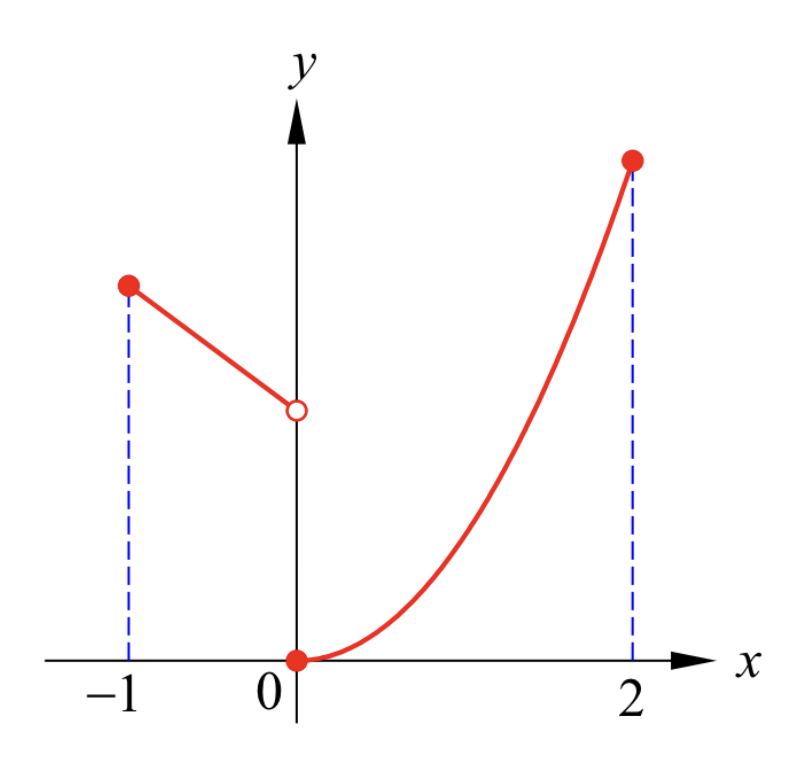
\includegraphics[scale=0.2]{Picture42.png}
\caption{The piecewise continuous function defined in Example \ref{ex230221_10}.\fa}\label{figure42}
\end{figure}
A special class of function that is bounded and piecewise continuous is the class of step functions. 
\begin{definition}{Step Functions}
We say that   $f:[a,b]\to\mathbb{R}$ is a step function if there is a partition $P_0=\{a_0, a_1, \ldots, a_k\}$ of $[a,b]$ such that for each $1\leq i\leq k$, $f:(a_{i-1}, a_i)\to\mathbb{R}$ is a constant function.
\end{definition}
By previous theorem, a step function is Riemann integrable. In fact, it is easy to compute its integral.
\begin{proposition}{}
Let $P_0=\{a_0, a_1, \ldots, a_k\}$ be a partition of $[a,b]$, and let $f:[a,b]\to\mathbb{R}$ be a step function such that for $1\leq i\leq k$,
\[f(x)=c_i,\quad\text{when}\quad a_{i-1}< x< a_i.\] Then $f:[a,b]\to\mathbb{R}$  is Riemann integrable  and
\[\int_a^b f=\sum_{i=1}^k c_i(a_i-a_{i-1}).\]
\end{proposition}

\begin{example}[label=ex230221_14]{}
Let $f:[0,5]\to\mathbb{R}$ be the function defined as 
\begin{align*}
f(x)=\begin{cases} 1,\quad &\text{if}\;0\leq x\leq \di 1,\\
\di\left\lfloor 5/x\right\rfloor,\quad &\text{if}\; \di 1< x\leq 5.\end{cases}
\end{align*}Show that $f$ is Riemann integrable and find $\di\int_0^5 f$. 
\end{example}


\begin{solution}{Solution}
The function $f$ is given explicitly by
\begin{align*}
f(x)=\begin{cases} 1,\quad &\text{if}\hspace{0.7cm} 0\leq x\leq \di 1,\\4,\quad &\text{if}\hspace{0.7cm} \di 1< x\leq 5/4,\\
3,\quad &\text{if}\;\; \di 5/4< x\leq 5/3,\\
2,\quad &\text{if}\; \;\di 5/3<x\leq 5/2,\\
1,\quad &\text{if}\; \;\di 5/2< x\leq 5.
 \end{cases}
\end{align*}
This is a step function. Hence, it is integrable, and
\[\int_0^5f=1\times 1+4\times \frac{1}{4}+3\times \frac{5}{12}+2\times\frac{5}{6}+1\times\frac{5}{2}=\frac{89}{12}.\]
\end{solution}
 \begin{figure}[ht]
\centering
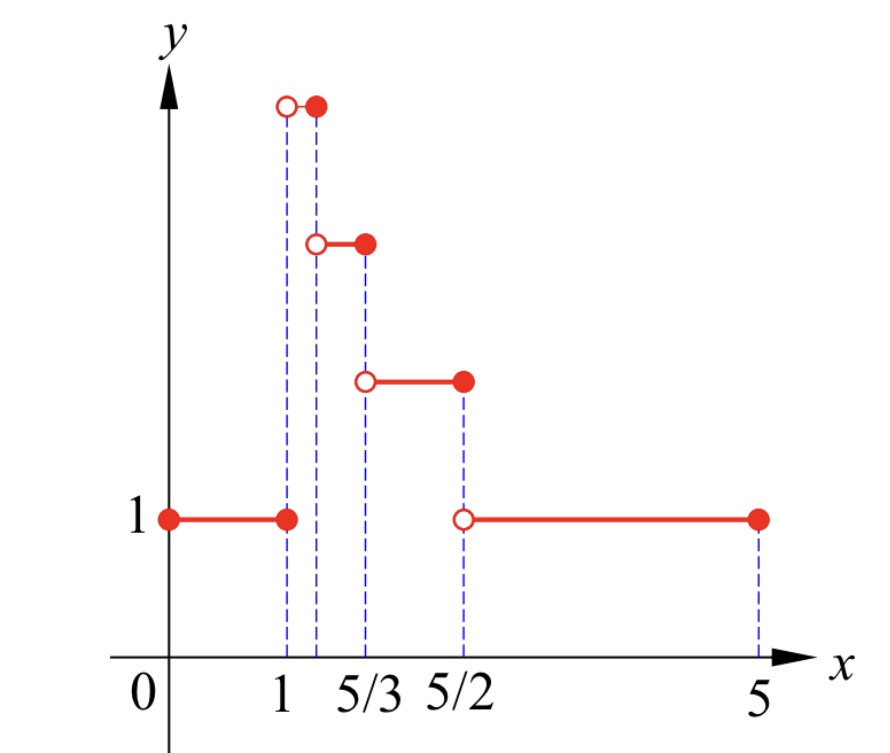
\includegraphics[scale=0.2]{Picture43.png}
\caption{The   function defined in Example \ref{ex230221_14}.\fa}\label{figure43}
\end{figure}

The following theorem shows that  monotonic functions are also Riemann integrable.
\begin{theorem}{}
If  $f:[a,b]\to\mathbb{R}$   is a monotonic function, then   it  is Riemann integrable.
\end{theorem}
\begin{myproof}{Proof} Without loss of generality, assume that $f:[a,b]\to\mathbb{R}$ is an increasing function. If $P=\{x_i\}_{i=0}^k$ is a partition of $[a,b]$, then for any $1\leq i\leq k$,
\[m_i=\inf_{x_{i-1}\leq x\leq x_i}f(x)=f(x_{i-1}),\hspace{1cm}M_i=\inf_{x_{i-1}\leq x\leq x_i}f(x)=f(x_i).\]
Therefore,
\[U(f,P)-L(f,P)=\sum_{i=1}^n\left(f(x_i)-f(x_{i-1}\right)(x_i-x_{i-1}).\]
For each positive integer $n$, let $P_n$ be the regular partition of $[a, b]$ into $n$ intervals. Then
\begin{align*}U(f, P_n)-L(f, P_n)&=\frac{b-a}{n}\sum_{i=1}^n\left(f(x_i)-f(x_{i-1})\right)\\&=\frac{(b-a)\left(f(b)-f(a)\right)}{n}.\end{align*}
\bp
This implies that
\[\lim_{n\to \infty}\left(U(f, P_n)-L(f, P_n)\right)=\lim_{n\to \infty}\frac{(b-a)\left(f(b)-f(a)\right)}{n}=0.\]
In other words, $\{P_n\}$ is an Archimedes sequence of partitions for $f$. By the Archimedes-Riemann theorem, this proves that $f$ is Riemann integrable.
\end{myproof}
\begin{example}{}
Let $f:[0,1]\to\mathbb{R}$ be the function defined by $f(0)=1$, and for each positive integer $n$, 
\[f(x)=1-\frac{1}{n+1},\hspace{1cm}\text{when}\; \frac{1}{n+1}<x\leq\frac{1}{n}.\]
One can verify that $f:[0,1]\to\mathbb{R}$ is a decreasing function. Hence, it is Riemann integrable.
However, $f$ is not a piecewise continuous function, since it has discontinuities at infinitely many points. 
\end{example}

The Riemann integrability of a function implies the Riemann integrability of its absolute value.
\begin{theorem}[label=230221_15]{}
Let $f:[a,b]\to\mathbb{R}$   be a bounded function. If  $f:[a,b]\to\mathbb{R}$ is Riemann integrable, then the function  $|f|:[a,b]\to\mathbb{R}$ is Riemann integrable.
\end{theorem}

\begin{myproof}{Proof}We will first prove the following: For any $c$ and $d$ in $[a,b]$ with $c<d$,
\begin{equation}\label{eq230221_19}\sup_{c\leq x\leq d}|f(x)|-\inf_{c\leq x\leq d}|f(x)|\leq  \sup_{c\leq x\leq d}f(x) -\inf_{c\leq x\leq d}f(x).\end{equation}
 There are two sequences of points $\{u_n\}$ and $\{v_n\}$ in $[c,d]$ such that
\[\lim_{n\to\infty}|f(u_n)|=\inf_{c\leq x\leq d}|f(x)|,\hspace{1cm}\lim_{n\to\infty}|f(v_n)|=\sup_{c\leq x\leq d}|f(x)|.\]\bp
Since $u_n$ and $v_n$ are points in $[c,d]$, we find that
\[|f(v_n)|-|f(u_n)|\leq|f(v_n)-f(u_n)|\leq \sup_{c\leq x\leq d}f(x) -\inf_{c\leq x\leq d}f(x).\]
Passing to the $n\to\infty$ limit, we obtain \eqref{eq230221_19}.

 
 
Now, given $\varepsilon>0$, since $f:[a,b]\to\mathbb{R}$ is Riemann integrable, there is a partition $P=\{x_i\}_{i=0}^k$ of $[a,b]$ such that 
\[U(f,P)-L(f,P) <\varepsilon.\]
But then \begin{align*}
&U(|f|,P)-L(|f|,P)\\&=\sum_{i=1}^n\left(\sup_{x_{i-1}\leq x\leq x_i}|f(x)|-\inf_{x_{i-1}\leq x\leq x_i}|f(x)|\right)(x_i-x_{i-1})\\
&\leq \sum_{i=1}^n\left(\sup_{x_{i-1}\leq x\leq x_i}f(x)-\inf_{x_{i-1}\leq x\leq x_i}f(x)\right)(x_i-x_{i-1})\\&=U(f,P)-L(f,P)<\varepsilon.\end{align*}This prove that $|f|:[a,b]\to\mathbb{R}$ is Riemann integrable.
\end{myproof}

\begin{figure}[ht]
\centering
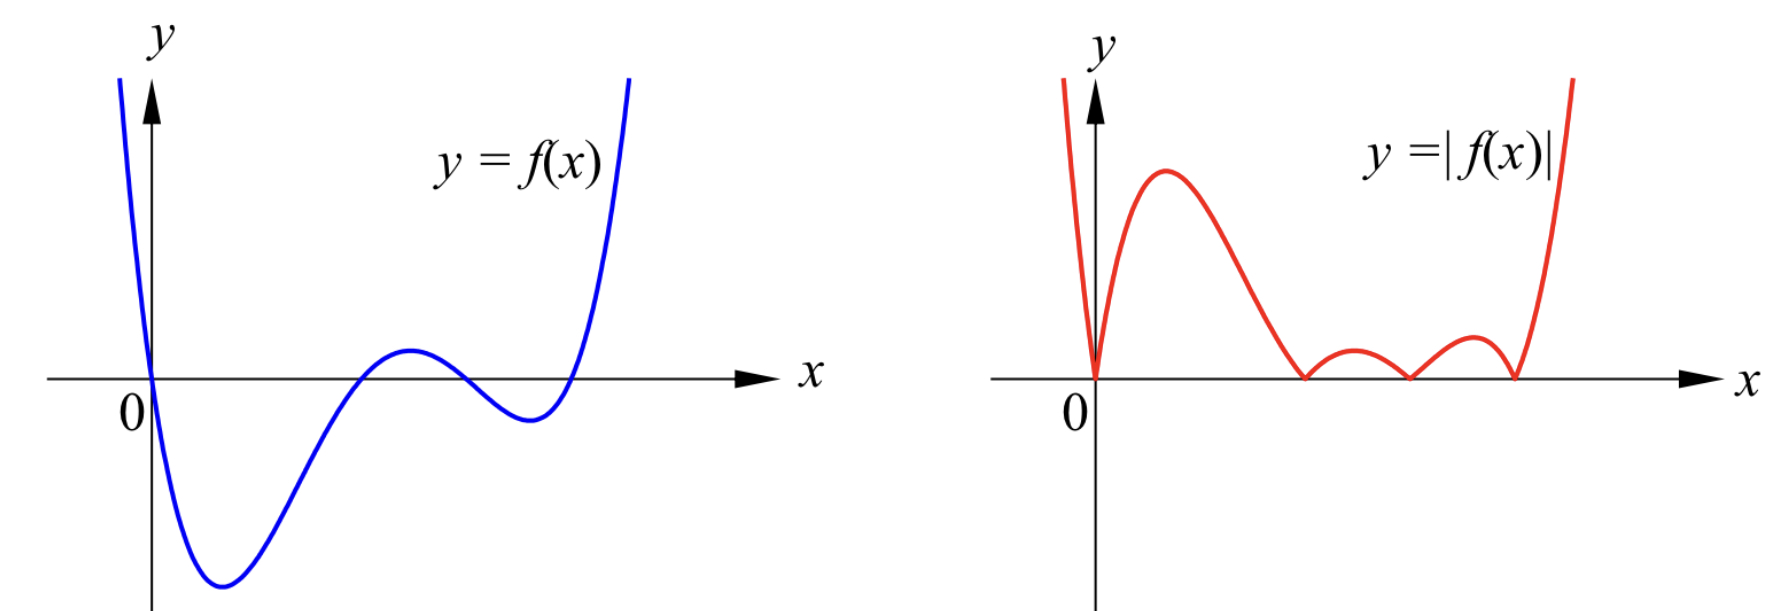
\includegraphics[scale=0.2]{Picture44.png}
\caption{A function $y=f(x)$ and its absolute value $y=|f(x)|$.\fa}\label{figure44}
\end{figure}
\begin{remark}{}
The converse of Theorem \ref{230221_15} is not true. Namely, if a function $f:[a,b]\to\mathbb{R}$ is bounded, $|f|:[a,b]\to\mathbb{R}$ is Riemann integrable does not imply that $f:[a,b]\to\mathbb{R}$ is Riemann integrable. For a counter example, consider the function $f:[0,1]\to\mathbb{R}$ defined as
\[f(x)=\begin{cases} 1,\quad &\text{if $x$ is rational},\\-1,\quad & \text{if $x$ is irrational}.\end{cases} \]
One can prove that $f:[0,1]\to\mathbb{R}$ is not integrable, exactly the same way as in Example \ref{230220_9}. On the other hand, since $|f|:[0,1]\to\mathbb{R}$ is a constant function, it is Riemann integrable.
\end{remark}


 The following theorem says that the product of Riemann integrable functions is Riemann integrable.
\begin{theorem}{}
Let $f:[a,b]\to\mathbb{R}$ and  $g:[a,b]\to\mathbb{R}$ be bounded functions. If  $f:[a,b]\to\mathbb{R}$ and  $g:[a,b]\to\mathbb{R}$ are Riemann integrable, then the function  $(fg):[a,b]\to\mathbb{R}$ is also Riemann integrable.
\end{theorem}
\begin{myproof}{Proof}We will apply Lemma \ref{230220_10} to prove the Riemann integrability of the function  $h=(fg):[a,b]\to\mathbb{R}$.
Since  $f:[a,b]\to\mathbb{R}$ and  $g:[a,b]\to\mathbb{R}$ are bounded functions, there is a positive number $M$ so that 
\[|f(x)|\leq M\quad\text{and}\quad|g(x)|\leq M\hspace{1cm}\text{for all}\;x\in [a,b].\]
We claim that for any $c$ and $d$ in $[a,b]$ with $c<d$,
\begin{equation}\label{230524_1}\begin{split}&\sup_{c\leq x\leq d}h(x)-\inf_{c\leq x\leq d}h(x)\\&\leq M\left(\sup_{c\leq x\leq d}f(x)-\inf_{c\leq x\leq d}f(x)+\sup_{c\leq x\leq d}g(x)-\inf_{c\leq x\leq d}g(x)\right).\end{split}\end{equation}\bp
 There are two sequences of points $\{u_n\}$ and $\{v_n\}$ in $[c,d]$ such that
\[\lim_{n\to\infty}h(u_n)=\inf_{c\leq x\leq d}h(x),\hspace{1cm}\lim_{n\to\infty}h(v_n)=\sup_{c\leq x\leq d}h(x).\] 
Notice that
\begin{align*}
|h(v_n)-h(u_n)|&=|g(v_n)(f(v_n)-f(u_n))+f(u_n)(g(v_n)-g(u_n))|\\
&\leq |g(v_n)||f(v_n)-f(u_n)|+|f(u_n)||g(v_n)-g(u_n)|\end{align*}  Since $u_n$ and $v_n$ are in $[c,d]$, we find that
\[|f(v_n)-f(u_n)|\leq \sup_{c\leq  x\leq d}f(x)-\inf_{c\leq x\leq d}f(x),\]
\[|g(v_n)-g(u_n)|\leq \sup_{c\leq  x\leq d}g(x)-\inf_{c\leq x\leq d}g(x).\]
Therefore,
\begin{align*}
&|h(v_n)-h(u_n)|\\&\leq M\left(\sup_{c\leq  x\leq d}f(x)-\inf_{c\leq x\leq d}f(x)+\sup_{c\leq x\leq d}g(x)-\inf_{c\leq x\leq d}g(x)\right).
\end{align*}Passing to the $n\to\infty$ limit gives \eqref{230524_1}.

Now given $\varepsilon>0$, there are partitions $P_1$ and $P_2$ of $[a,b]$ such that
\begin{gather*}U(f,P_1)-L(f,P_1)<\frac{\varepsilon}{2M},\\
U(g,P_2)-L(g,P_2)<\frac{\varepsilon}{2M}.\end{gather*}
Let $P^*=\{x_0, x_1, \ldots, x_k\}$ be  a common refinement of $P_1$ and $P_2$. Then
\begin{gather*}
U(f,P^*)-L(f,P^*)<\frac{\varepsilon}{2M},\\
U(g,P^*)-L(g,P^*)<\frac{\varepsilon}{2M}.\end{gather*}


 
\bp
 It follows that
\begin{align*}
&U(h,P^*)-L(h,P^*)\\&=\sum_{i=1}^k\left(\sup_{x_{i-1}\leq x\leq x_i}h(x)-\inf_{x_{i-1}\leq x\leq x_i}h(x)\right)(x_i-x_{i-1})\\
&\leq M\sum_{i=1}^k\left(\sup_{x_{i-1}\leq x\leq x_i}f(x)-\inf_{x_{i-1}\leq x\leq x_i}f(x)\right)(x_i-x_{i-1})\\
&\quad +M\sum_{i=1}^k\left(\sup_{x_{i-1}\leq x\leq x_i}g(x)-\inf_{x_{i-1}\leq x\leq x_i}g(x)\right)(x_i-x_{i-1})\\
&=M\left(U(f,P^*)-L(f,P^*)+U(g,P^*)-L(g,P^*)\right)\\
&<M\times\left(\frac{\varepsilon}{2M}+\frac{\varepsilon}{2M}\right)=\varepsilon.
\end{align*}This proves that $(fg):[a,b]\to\mathbb{R}$ is   Riemann integrable.
\end{myproof}
\vp
\noindent
{\bf \large Exercises  \thesection}
\setcounter{myquestion}{1}
 
\begin{question}{\themyquestion}
Given that $f:[-1,1]\to\mathbb{R}$ is the function defined by
\[f(x)=\begin{cases} \di \sin\left(\frac{4}{x}\right),\quad &\text{if}\;x\neq 0,\\
0,\quad &\text{if}\;x= 0.\end{cases}\]Explain why $f:[-1,1]\to\mathbb{R}$ is Riemann integrable.
\end{question}
\atc

\begin{question}{\themyquestion}
Let $f:[a,b]\to\mathbb{R}$ be a bounded function. If $f:[a,b]\to\mathbb{R}$ is Riemann integrable, show that
\[\left|\int_a^b f(x)dx\right|\leq \int_a^b |f(x)|dx.\]
\end{question}
\atc
\begin{question}{\themyquestion}
Let $f:[0,6]\to\mathbb{R}$ be the function defined as 
\begin{align*}
f(x)=\begin{cases} -2,\quad &\text{if}\;0\leq x<\di 1,\\
\di\left\lfloor 4/x\right\rfloor,\quad &\text{if}\; \di 1\leq x\leq 6.\end{cases}
\end{align*}Show that $f$ is Riemann integrable and find $\di\int_0^6 f$. 
\end{question}
\atc



\begin{question}{\themyquestion}
Let $f:\mathbb{R}\to\mathbb{R}$ be the function defined as
\[f(x)=\left(x-\lfloor x\rfloor\right)^2.\]
Explain why the function $f$ is Riemann integrable on any closed and bounded interval $[a,b]$.
\end{question}

\atc

\begin{question}[label=ex230224_7]{\themyquestion}
Let $f:[a,b]\to\mathbb{R}$ and $g:[a,b]\to\mathbb{R}$ be bounded functions. Define the function
$h:[a,b]\to\mathbb{R}$ by
\[h(x)=\max\{f(x), g(x)\}.\]
\begin{enumerate}[(a)]
\item
Show that
\[h=\frac{f+g+|f-g|}{2}.\]
\item If  $f:[a,b]\to\mathbb{R}$ and $g:[a,b]\to\mathbb{R}$ are Riemann integrable, show that $h:[a,b]\to\mathbb{R}$ is also Riemann integrable.
\end{enumerate}
\end{question}
\atc
 \begin{question}{\themyquestion\;\;[Cauchy Schwarz Inequality]}
Let $f:[a,b]\to\mathbb{R}$ and $g:[a,b]\to\mathbb{R}$ be bounded functions that are Riemann integrable. Prove that
\[\left(\int_a^b f(x)g(x)dx\right)^2\leq \left(\int_a^bf(x)^2dx\right)\left(\int_a^bg(x)^2dx\right).\]
\end{question}
\vp
\section{The Fundamental Theorem of Calculus}\label{sec4.4}
In this section, we prove the fundamental theorem of calculus, which gives a relation between integration and differentiation. It also provides a useful method to compute integrals of certain functions. 
We first prove a few results about integrals.

 Given that a function $f:[a,b]\to\mathbb{R}$ is bounded and Riemann integrable on $[a,b]$, it is Riemann integrable on any interval $[c,d]$ that is contained in the interval $[a,b]$. Thus,  we can define a new function $F:[a,b]\to\mathbb{R}$ by
\[F(x)=\int_a^x f(u)du.\]
By definition, $F(a)=0$. 
For any $c$ and $d$ in $[a, b]$, one can check that
\[F(d)-F(c)=\int_a^df(u)du-\int_a^cf(u)du=\int_c^df(u)du.\]
The followng theorem says that  $F:[a,b]\to\mathbb{R}$ is a continuous function.
\begin{theorem}[label=230222_11]{}
Let $f:[a,b]\to\mathbb{R}$ be a bounded function that is Riemann integrable, and let $F:[a,b]\to\mathbb{R}$ be the function defined by \[F(x)=\int_a^x f(u)du.\]Then $F:[a,b]\to\mathbb{R}$ is a Lipschitz function, and hence it is continuous.
\end{theorem}
\begin{myproof}{Proof}
It is sufficient to prove that $F:[a,b]\to\mathbb{R}$ is Lipschitz. The continuity follows. Since $f:[a,b]\to\mathbb{R}$ is bounded, there is a positive constant $M$ such that
\[|f(x)|\leq M\hspace{1cm}\text{for all}\;x\in [a,b].\]\bp

For any $x_1$ and $x_2$ in $[a,b]$ with $x_1<x_2$, we have
\[ F(x_2)-F(x_1)= \int_{x_1}^{x_2}f(u)du.\]
Therefore,
\begin{align*}
|F(x_2)-F(x_1)|&=\left|\int_{x_1}^{x_2}f(u)du\right|\leq \int_{x_1}^{x_2}|f(u)|du\\&\leq \int_{x_1}^{x_2}Mdu=M(x_2-x_1)=M|x_2-x_1|.
\end{align*}This proves that $F:[a,b]\to\mathbb{R}$ is a Lipschitz function wth Lipschitz constant $M$. 
\end{myproof}


The next is a mean value theorem for integrals.
\begin{theorem}{Mean Value Theorem for Integrals}
Let $f:[a,b]\to\mathbb{R}$ be a continuous function. Then there exists $c$ in $[a,b]$ such that
\[\frac{1}{b-a}\int_a^bf(x)dx=f(c).\]
\end{theorem}This theorem is known as the mean value theorem since 
\[\frac{1}{b-a}\int_a^bf(x)dx\]can be interpreted as the average of the values of $f$ over the interval $[a,b]$. 
\begin{myproof}{Proof}
Since $f:[a,b]\to\mathbb{R}$ is a continuous function, the extreme value theorem says that there are points $u$ and $v$ in $[a,b]$ such that
\[f(u)\leq f(x)\leq f(v)\hspace{1cm}\text{for all}\;x\in [a,b].\]This implies that
\[f(u)(b-a)\leq \int_a^b f(x)dx\leq f(v)(b-a).\]\bp

Therefore, the number
\[w=\frac{1}{b-a}\int_a^bf(x)dx\]satisfies
\[f(u)\leq w\leq f(v).\]
By intermediate value theorem, there is a point $c$ in $[a,b]$ such that $f(c)=w$. This gives
\[\frac{1}{b-a}\int_a^bf(x)dx=f(c).\]
\end{myproof}
In fact, one can argue that the number $c$ can be chosen to be in  $(a,b)$.  

\begin{example}[label=ex230222_5]{}
Let $f:[a,b]\to\mathbb{R}$ be a continuous function. If  $f(x)\geq m$ for all $x\in [a,b]$ and 
\[\int_a^b f(x)dx=m(b-a),\]prove that
\[f(x)=m\hspace{1cm}\text{for all}\;x\in [a,b].\]
\end{example}
\begin{solution}{Solution}
Let $g:[a,b]\to\mathbb{R}$ be the function $g(x)=f(x)-m$. Then $g:[a,b]\to\mathbb{R}$ is a continuous function and $g(x)\geq 0$ for all $x\in [a,b]$. Moreover,
\[\int_a^b g(x)dx=\int_a^b f(x)dx-\int_a^b mdx=0.\]
We want to show that $g(x)=0$ for all $x\in [a,b]$. Suppose to the contrary that there is a point $x_0$ in $[a,b]$ such that $g(x_0)\neq 0$. Then $g(x_0)>0$. Since $g$ is continuous, there exists a $\delta>0$ such that for all $x\in (x_0-\delta,x_0+\delta)\cap (a,b)$, 
\[g(x)>\frac{g(x_0)}{2}.\]\bs
Without loss of generality, assume that $\delta<\di\frac{b-a}{2}$. Then either $x_0-\delta>a$ or $x_0+\delta<b$. In any case, $(x_0-\delta,x_0+\delta)\cap (a,b)=(c,d)$ is an interval of length at least $\delta$. But then
\begin{align*}\int_a^b g(x)dx&=\int_{a}^cg(x)dx+\int_c^dg(x)dx+\int_d^bg(x)dx\\&\geq 0\times (c-a)+(d-c)\frac{g(x_0)}{2}+0\times (b-d)\\&=(d-c)\frac{g(x_0)}{2}>0,\end{align*}
which is a contradiction. Therefore, we must have $g(x)=0$ for all $x\in [a,b]$.
\end{solution}

\begin{remark}{}
In the mean value theorem for integrals, we can strengthen the theorem to have the point $c$  being a point in the open interval $(a,b)$. In the proof, we have shown that for $w=\di\int_a^b f(x)dx$,
 \[f(u)\leq w\leq f(v).\] Here $f(u)$ is the minimum value of $f:[a,b]\to\mathbb{R}$, and $f(v)$ is the maximum value. By Example \ref{ex230222_5}, if $w=f(u)$, then $f$ is a constant. In this case, we can take $c$ to be any point in $(a,b)$. If $w=f(v)$, the same reasoning as in Example \ref{ex230222_5} also shows that $f$ is a constant, and so $c$ also can be any point in $(a,b)$. If $w\neq f(u)$ and $w\neq f(v)$, then $c$ is a point strictly between $u$ and $v$, and thus it is strictly between $a$ and $b$.
\end{remark}

Now we turn to the fundamental theorem of calculus. Consider the case that an object is moving with speed $v(t)$ at time $t$. To find $s(t)$, the distance  travelled up to time $t$, we can partition the time interval $[0, t]$ into a finite number of subintervals $[0, t_1], [t_1, t_2], \ldots, [t_{k-1}, t_k]$, where $t_k=t$. For each time interval $[t_{i-1}, t_i]$, where $1\leq i\leq k$, take a point $t_i^*\in [t_{i-1}, t_i]$, and approximate the average speed over the time interval $[t_{i-1}, t_i]$ by the speed at time $t_i^*$, $v(t_i^*)$. Then the distance travelled up to time $t$ is approximately 
\[\sum_{i=1}^k v(t_i^*)(t_i-t_{i-1}).\]
We recognize that this is  a Riemann sum of the speed function $v(t)$. The distance travelled $s(t)$ should be calculated as the limit where the gap of the partition goes to zero. In other words,
\[s(t)=\int_0^t v(\tau)d\tau.\]In Chapter \ref{ch3}, we have motivated that $v(t)=s'(t)$. Hence, 
\[s(t)=\int_0^ts'(\tau)d\tau,\]which means that differentiation and integration are inverse processes of each other. The fundamental theorem of calculus gives a rigorous setting for this.
\begin{theorem}{Fundamental Theorem of Calculus I}
Let $f:[a,b]\to\mathbb{R}$ be a bounded function that is Riemann integrable, and let $F:[a,b]\to\mathbb{R}$ be the function defined by
\[F(x)=\int_a^xf(u)du.\]
If $x_0$ is a point in $ (a,b)$, and $f$ is continuous at $x_0$, then $F$ is differentiable at $x_0$ and
\[F'(x_0)=f(x_0).\]
\end{theorem}
 
\begin{myproof}{Proof of Fundamental Theorem of Calculus I}
We need to show that the limit
\[\lim_{h\to 0}\frac{F(x_0+h)-F(x_0)}{h}\] exists and is equal to $f(x_0)$. Given $\varepsilon>0$, since $f$ is continuous at $x_0$, there is a $\delta>0$ such that $(x_0-\delta,x_0+\delta)\subset (a,b)$ and 
\begin{equation}\label{eq230222_10}\left|f(x)-f(x_0)\right|<\frac{\varepsilon}{2}\hspace{1cm}\text{for all}\; x\in (x_0-\delta, x_0+\delta).\end{equation}
\bp
For $h\in (-\delta, \delta)$,
\begin{align*}
F(x_0+h)-F(x_0)-f(x_0)h&=\int_{x_0}^{x_0+h}f(u)du-f(x_0)h\\&=\int_{x_0}^{x_0+h}\left(f(u)-f(x_0)\right)du.\end{align*}
Eq. \eqref{eq230222_10} implies that
\[\left|F(x_0+h)-F(x_0)-f(x_0)h\right|\leq\frac{\varepsilon}{2}|h|.\]
Hence, if $h\in (-\delta, \delta)\setminus\{0\}$, 
\[\left|\frac{F(x_0+h)-F(x_0)}{h}-f(x_0) \right|\leq\frac{\varepsilon}{2}<\varepsilon.\]
This proves that
\[\lim_{h\to 0}\frac{F(x_0+h)-F(x_0)}{h}=f(x_0).\]
\end{myproof}
In fact, the point $x_0$ can be $a$ or $b$ if we consider one-sided derivatives.

\begin{example}[label=20230527]{}
Consider the piecewise continuous function $f:[0,2]\to\mathbb{R}$ given by 
\[f(x)=\begin{cases} -1,\quad&\text{if}\; 0\leq x<1,\\
2,\quad&\text{if}\; 1\leq x<2,\\
1,\quad &\text{if}\;\quad x=2.\end{cases}\]
We find that
\[F(x)=\int_0^x f(u)du=\begin{cases} -x,\quad&\text{if}\; 0\leq x<1,\\
2x-3,\quad&\text{if}\; 1\leq x\leq 2.\end{cases}\]\be
The function $F:[0,2]\to\mathbb{R}$ is   continuous.
For $x\in (0,1)$, $F$ is differentiable and $F'(x)=-1=f(x)$. For  $x\in (1,2)$, $F$ is differentiable and $F'(x)=2$. However, $F$ is not differentiable at $x=1$ since
\[\lim_{x\to 1^-}\frac{F(x)-F(1)}{x-1}=-1,\hspace{1cm}\lim_{x\to 1^+}\frac{F(x)-F(1)}{x-1}=2.\]
\end{example2}
\begin{figure}[ht]
\centering
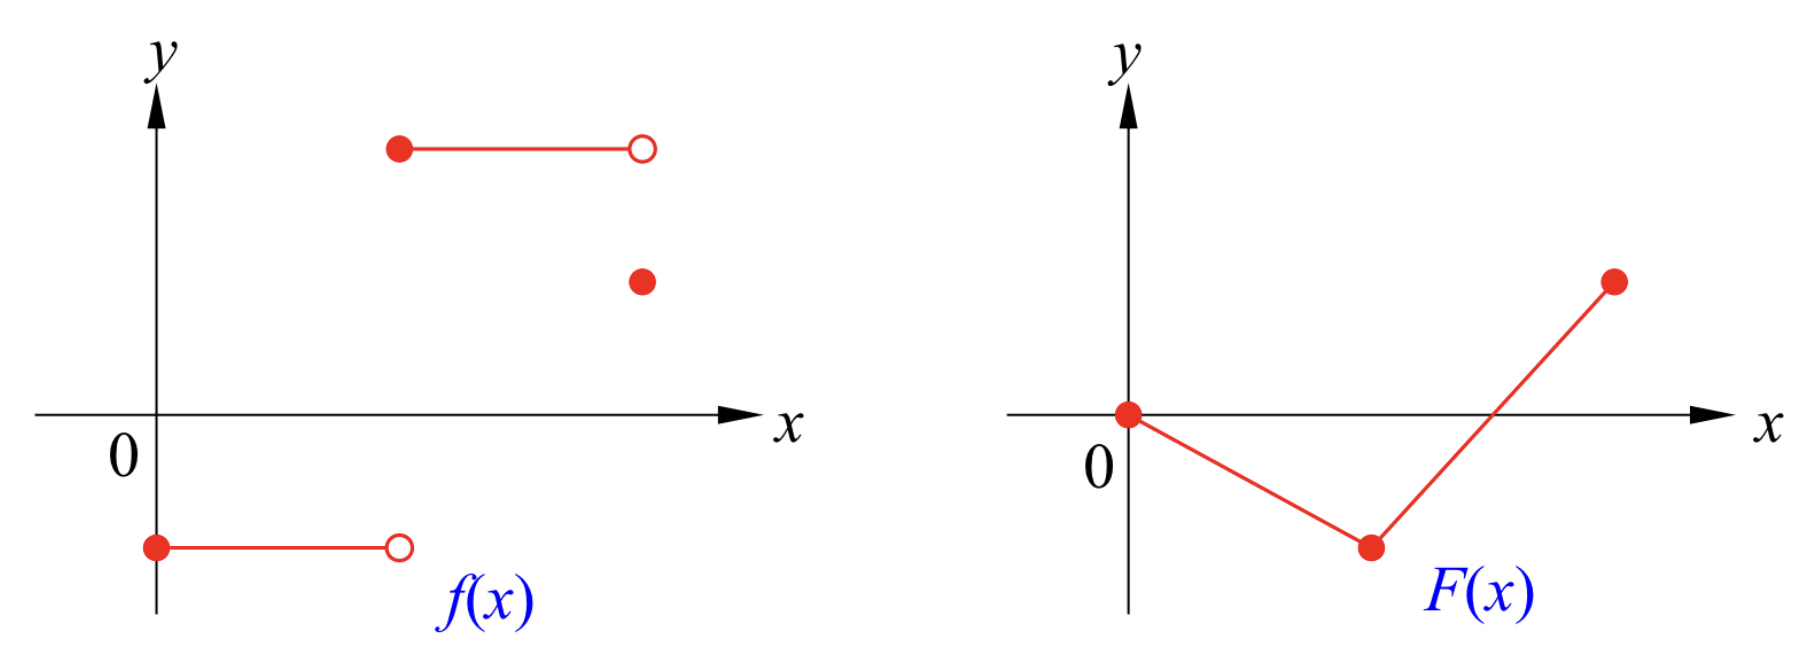
\includegraphics[scale=0.2]{Picture69.png}
\caption{The function  $f:[0,2]\to\mathbb{R}$  and  $F:[0,2]\to\mathbb{R}$ in Example \ref{20230527}.}\label{figure69}
\end{figure}
\begin{example}{}
Evaluate the following derivatives.
\begin{enumerate}[(a)]
\item
$\di\frac{d}{dx}\int_0^x\sin(u^2)du$
\item
$\di\frac{d}{dx}\int_x^{1}\sin(u^2)du$
\item
$\di\frac{d}{dx}\int_x^{x^2}\sin(u^2)du$
\end{enumerate}
\end{example}
\begin{solution}{Solution}
The function $f:\mathbb{R}\to\mathbb{R}$, $f(x)=\sin(x^2)$ is continuous. Hence, it is Riemann integrable over any closed and bounded intervals. Let
\[F(x)=\int_0^xf(u)du=\int_0^x\sin(u^2)du.\]\bs
 By fundamental theorem of calculus I, $F'(x)=f(x)=\sin(x^2)$.
\begin{enumerate}[(a)]
\item$\di \frac{d}{dx}\int_0^x\sin(u^2)du=\frac{d}{dx}F(x) =\sin (x^2)$.
\item $\di \frac{d}{dx}\int_x^{1}\sin(u^2)du=\frac{d}{dx}\left(F(1)-F(x)\right) =-F'(x)= -\sin(x^2)$.
\item $\di \frac{d}{dx}\int_x^{x^2}\sin(u^2)du=\frac{d}{dx}\left(F(x^2)-F(x)\right)=2xF'(x^2)-F'(x) $\\~$~\hspace{5cm}~$$=2x\sin(x^4)-\sin(x^2)$.
\end{enumerate}

\end{solution}

Now we turn to the second fundamental theorem of calculus, which provides a mean for   calculating integrals of continuous functions.
\begin{theorem}{Fundamental Theorem of Calculus II}
Let $F:[a,b]\to\mathbb{R}$ be a continuous function, and let $f:[a,b]\to\mathbb{R}$ be a bounded function that is continuous on $(a,b)$. If 
\[F'(x)=f(x)\hspace{1cm}\text{for all}\;x\in (a,b),\]
Then
\[\int_a^b f(x)dx=F(b)-F(a).\]
\end{theorem}
Recall that if the functions $F(x)$ and $f(x)$ are related by
\[F'(x)=f(x)\hspace{1cm}\text{for all}\;x\in (a,b),\]$F$ is called an antiderivative of $f$. Hence, the fundamental theorem of calculus II states that if the function $f:(a,b)\to\mathbb{R}$ is continuous and it has an antiderivative $F(x)$ which can be extended to a continuous function $F:[a,b]\to\mathbb{R}$, then 
\[\int_a^bf(x)dx=\left[ F(x)\right]_{ a}^{ b}=F(b)-F(a).\]
We will present two proofs of the fundamental theorem of calculus II. The first one uses fundamental theorem of calculus I.
\begin{myproof}{First  Proof of Fundamental Theorem of Calculus II}
Since $f:[a,b]\to\mathbb{R}$ is a bounded function that is continuous on $(a,b)$, it is integrable over any subinterval of $[a,b]$. Let $G:[a,b]\to\mathbb{R}$ be the function defined by
\[G(x)=\int_a^xf(u)du.\]By default, $G(a)=0$.  By Theorem \ref{230222_11}, $G$ is continuous on $[a,b]$.  By fundamental theorem of calculus I, 
\[G'(x)=f(x)\hspace{1cm} \text{for all}\;x\in (a,b).\]Hence, $F:[a,b]\to\mathbb{R}$ and $G:[a,b]\to\mathbb{R}$ are continuous functions satisfying
\[G'(x)=F'(x)\hspace{1cm} \text{for all}\;x\in (a,b).\] By Theorem \ref{thm230215_3}, there is a constant $C$ such that 
\[G(x)=F(x)+C.\]
Since $G(a)=0$, we find that 
$C=-F(a)$. Therefore, 
\[G(x)=F(x)-F(a),\]and so
\[\int_a^bf(x)dx=G(b)=F(b)-F(a).\]
\end{myproof}
In different textbooks, the ordering of the two fundamental theorem of calculus might be different. One can use one to deduce the other. This is why a   proof of the fundamental theorem of calculus II without using the fundamental theorem of calculus I is of interest.


\begin{myproof}{Second Proof of Fundamental Theorem of Calculus II}
Here we use the Lagrange mean value theorem. Since $f:[a,b]\to\mathbb{R}$ is a bounded function that is continuous on $(a,b)$, it is integrable. Now if $P=\{x_i\}_{i=0}^k$ is a partition of $[a,b]$, for each $1\leq i\leq k$, the mean value theorem implies that there is a $\xi_i\in (x_{i-1}, x_i)$ such that
\[F(x_i)-F(x_{i-1})=F'(\xi_i)(x_i-x_{i-1})=f(\xi_i)(x_i-x_{i-1}).\]
Summing over $i$ gives
\[F(b)-F(a)=\sum_{i=1}^k\left(F(x_i)-F(x_{i-1})\right)=\sum_{i=1}^k f(\xi_i)(x_i-x_{i-1})=R(f,P,A),\]where $A=\{\xi_i\}_{i=1}^k$. Since
\[L(f,P)\leq R(f,P,A)\leq U(f,P),\]we find that
\[L(f,P)\leq F(b)-F(a)\leq U(f,P).\]
Notice that this is true for any partition $P$ of $[a,b]$. By definitions of the lower integral and the upper integral, we find that
\[\underline{\int_a^b}f\;\leq\;F(b)-F(a)\;\leq\;\overline{\int_a^b}f.\]
Since $f:[a,b]\to\mathbb{R}$ is Riemann integrable, the lower integral and the upper integral are the same. Thus,
\[\int_a^b f=\underline{\int_a^b}f=\overline{\int_a^b}f=F(b)-F(a).\]
 

\end{myproof}


We can relax the conditions in the fundamental theorem of calculus II to let $f$ to be a piecewise continuous function.
\begin{corollary}{Generalized Fundamental Theorem of Calculus II}
 Let $S=\{a_0, a_1, \ldots, a_k\}$ be a finite subset of $[a,b]$ that contains $a$ and $b$, and let $f:[a,b]\to\mathbb{R}$ be a bounded function that is continuous on $[a,b]\setminus S$. If $F:[a,b]\to\mathbb{R}$ is a continuous function, differentiable on $[a,b]\setminus S$, and
\[F'(x)=f(x)\hspace{1cm}\text{for all}\;x\in [a,b]\setminus S,\] then
\[\int_a^b f(x)dx=F(b)-F(a).\]
\end{corollary}
\begin{myproof}{Proof}
We can assume that
\[a=a_0<a_1<\ldots<a_k=b.\]
Since $f:[a,b]\to\mathbb{R}$ is bounded and piecewise continuous, it is Riemann integrable. Moreover, by the generalized additivity theorem, we have
\[\int_a^bf(x)dx=\sum_{i=1}^k\int_{a_{i-1}}^{a_i}f(x)dx.\]
Applying the fundamental theorem of calculus II to each of the integrals $\di \int_{a_{i-1}}^{a_i}f(x)dx$, we find that
\[\int_a^b f(x)dx=\sum_{i=1}^k (F(a_i)-F(a_{i-1}))=F(b)-F(a).\]This completes the proof.
Note that it is crucial here that $F$ is continuous on $[a,b]$.
\end{myproof}

As is well known, the fundamental theorem of calculus provides a practical method for computing integrals of  functions that have antiderivatives. 
\begin{example}
{}
Compute the integral of the piecewise continuous function   $f:[-1, 2]\to\mathbb{R}$,
\[f(x)=\begin{cases} 2-x,\quad &\text{if}\; -1\leq x<0,\\
x^2,\quad &\text{if}\; \quad 0\leq x\leq 2,\end{cases}\] that is defined in Example \ref{ex230221_10}. 
\end{example}
\begin{solution}{Solution}
Using additivity,
\[\int_{-1}^2f(x)dx=\int_{-1}^0f(x)dx+\int_0^2f(x)dx.\]
Using fundamental theorem of calculus II, 
\[\int_{-1}^0f(x)dx=\int_{-1}^0(2-x)dx=\left[2x-\frac{x^2}{2}\right]_{-1}^0=0-\left(-\frac{5}{2}\right)=\frac{5}{2},\]
\[\int_0^2f(x)dx=\int_0^2x^2dx=\left[\frac{x^3}{3}\right]_0^2=\frac{8}{3}-0=\frac{8}{3}.\]
Hence,
\[\int_{-1}^2f(x)dx=\frac{5}{2}+\frac{8}{3}=\frac{31}{6}.\]

\end{solution}

\begin{remark}{Alternative Proof of Mean Value Theorem for Integrals}
Using the fundamental theorem of calculus, we can give an alternative proof of the mean value theorem for integrals as follows. Since the function $f:[a,b]\to\mathbb{R}$ is continuous, the function $F:[a,b]\to\mathbb{R}$ defined by
\[F(x)=\int_a^xf(u)du\] is continuous on $[a,b]$, differentiable on $(a,b)$, and $F'(x)=f(x)$ for all $x\in (a,b)$. By Lagrange mean value theorem, there is a $c\in (a,b)$ such that
\[\frac{1}{b-a}\int_a^bf(x)dx=\frac{F(b)-F(a)}{b-a}=F'(c)=f(c).\]
 
\end{remark}

Finally, we can prove the existence and uniqueness theorem mentioned in Chapter \ref{ch3}, Theorem \ref{thm230217_3}.
\begin{theorem}[label=thm230222_13]{Existence and Uniqueness Theorem}
Let $(a,b)$ be an open interval that contains the point $x_0$, and let $y_0$ be any real number.  Given that $f:(a,b)\to\mathbb{R}$ is a continuous function, there exists a unique differentiable function $F:(a,b)\to\mathbb{R}$ such that \[F'(x)=f(x)\quad \text{for all}\;x\in (a, b), \hspace{1cm}F(x_0)=y_0.\]
\end{theorem}
\begin{myproof}{Proof}
As we mentioned before, the uniqueness follows from the identity criterion. For the existence, notice that $f$ is continuous on any closed and bounded interval that is contained in $(a,b)$. Hence, we can define the function $F:(a,b)\to\mathbb{R}$ by
\[F(x)=\int_{x_0}^xf(u)du+y_0.\] 
Then $F(x_0)=y_0$ by default. By fundamental theorem of calculus, $F'(x)=f(x)$ for all $x\in (a,b)$.
\end{myproof}


Let us look at some other examples how integrals can be applied.  
\begin{example}{}
Find the limit 
\[\lim_{n\to\infty}\frac{1}{n}\sum_{k=1}^n\sin\left(\frac{\pi k}{n}\right).\]
\end{example}
\begin{solution}{Solution}
We try to identify \[\frac{1}{n}\sum_{k=1}^n\sin\left(\frac{\pi k}{n}\right)\] as a Riemann sum. For $1\leq k\leq n$, let $\xi_k=\di\frac{\pi k}{n}$.  These are equally spaced points in the interval $[0, \pi]$. This motivates us to define the function $f:[0,\pi]\to\mathbb{R}$, $f(x)=\sin x$. Since $f$ is a continuous function, it is Riemann integrable. Let $P_n$ be the regular partition of $[0,\pi]$ into $n$ intervals. Then with $A_n=\{\xi_k\}_{k=1}^n$, we have
\[R(f,P_n,A_n)=\sum_{k=1}^n\sin \left(\frac{\pi k}{n}\right)\frac{\pi }{n}.\]Since $f$ is Riemann integrable,
\[\lim_{n\to\infty}R(f, P_n, A_n)=\int_0^{\pi}f(x)dx.\]
By fundamental theorem of calculus,
\[\int_0^{\pi}f(x)dx=\int_0^{\pi}\sin xdx=\left[-\cos x\right]_0^{\pi}=2.\]
Therefore,
\[\lim_{n\to\infty}\frac{1}{n}\sum_{k=1}^n\sin\left(\frac{\pi k}{n}\right)=\frac{1}{\pi} \lim_{n\to\infty}R(f, P_n, A_n)=\frac{2}{\pi}.\]
\end{solution}
\vp
\noindent
{\bf \large Exercises  \thesection}
\setcounter{myquestion}{1}

 \begin{question}{\themyquestion}
Evaluate the following derivatives.
\begin{enumerate}[(a)]
\item
$\di\frac{d}{dx}\int_0^xe^{u^2}du$
\item
$\di\frac{d}{dx}\int_x^{1}\cos(u^2)du$
\item
$\di\frac{d}{dx}\int_x^{x^3}\sqrt{2+\sin u}\;du$
\end{enumerate}
\end{question}
\atc

 \begin{question}{\themyquestion}
Let $f:[-2, 6]\to\mathbb{R}$ be the function defined by
\[f(x)=\begin{cases} x^2-x,\quad & \text{if}\; -2\leq x<1,\\ \di x-\frac{1}{x},\quad &\text{if}\;\quad 1\leq x\leq 6.\end{cases} \]
Find a continuous function $F:[-2,6]\to\mathbb{R}$ such that $F$ is differentiable on $(-2,6)$, $F(0)=0$, and 
\[F'(x)=f(x)\hspace{1cm}\text{for all}\;x\in (-2,6).\]

\end{question}
\atc


 \begin{question}{\themyquestion}
Find the limit 
\[\lim_{n\to\infty}\frac{1^7+2^7+\cdots+n^7}{n^8}.\]
\end{question}
\atc
 \begin{question}{\themyquestion}
Find the limit 
\[\lim_{n\to\infty}\frac{1}{n}\sum_{k=1}^n\cos^2\left(\frac{2\pi k}{n}\right).\]
\end{question}
\vp





\section{Integration by Substitution and Integration by Parts}\label{sec4.5}


In this section, we prove the integration by substitution formula and integration by parts formula. We will only deal with the case where the function that we are integrating is continuous in the interior of the integration interval. For general case where the function is piecewise continuous, one can apply the additivity theorem.

\subsection{Integration by Substitution}
\begin{theorem}[label=230223_5]{Integration by Substitution}
Let  $g:[a,b]\to\mathbb{R}$ be a function that satisfies the following conditions:
\begin{enumerate}[(i)]
\item $g$ is continuous and one-to-one on $[a,b]$;
\item $g$  is continuously differentiable on $(a,b)$;
\item $g'(x)$ is bounded on $(a,b)$.
\end{enumerate}  Then $g  $ maps the interval $[a,b]$ onto  a closed and bounded interval $[c,d]$ with end points $g(a)$ and $g(b)$.   If $f:[c,d]\to\mathbb{R}$ is a   function that is   bounded and continuous on $(c,d)$, then the function $h:[a,b]\to \mathbb{R}$,
\[h(x)=f(g(x))g'(x)\]is  Riemann integrable and
\begin{equation}\label{eq230223_1}\int_a^bh(x)dx=\int_a^b f(g(x))g'(x)dx=\int_{g(a)}^{g(b)}f(u)du.\end{equation}
This is equivalent to
\begin{equation}\label{eq230223_2}\int_c^d f(u)du=\int_a^bf(g(x))|g'(x)|dx.\end{equation}
\end{theorem}
The function $g:[a,b]\to\mathbb{R}$ that satisfies all the three given conditions defines  a \emph{smooth} change of variables $u=g(x)$ from $x$ to $u$, in the sense that $g$ is continuously differentiable on $(a,b)$. 

\begin{myproof}{Proof}
Since $g$ is one-to-one, we have $g((a,b))\subset (c,d)$. Therefore, the function $h:[a,b]\to\mathbb{R}$, $h(x)=f(g(x))g'(x)$ is continuous and bounded on $(a,b)$, and hence, it is Riemann integrable.  For any $x\in [a,b]$, let
\begin{gather*}H_1(x) =\int_a^xh(u)du=\int_a^x f(g(u))g'(u)du,\\
F(x)=\int_c^xf(u)du,\\H_2(x) =\int_{g(a)}^{g(x)}f(u)du=F(g(x))-F(g(a)).\end{gather*}
Then $H_1(a)=H_2(a)=0$.
By fundamental theorem of calculus, $H_1$ and $H_2$ are differentiable on $(a,b)$, and for any $x\in (a,b)$,
\[H_1'(x)=h(x)=f(g(x))g'(x),\hspace{1cm} H_2'(x)=f(g(x))g'(x).\]
 Since $H_1'(x)=H_2'(x)$ for all $x\in (a,b)$, and $H_1(a)=H_2(a)$, we conclude that
$H_1(x)=H_2(x)$ for all $x\in [a,b]$. Namely,
\[\int_a^b f(g(x))g'(x)dx=\int_{g(a)}^{g(b)}f(u)du.\]
From this, we see that integration by substitution is just the inverse of the chain rule for differentiation.
To prove the equivalence of \eqref{eq230223_1} and \eqref{eq230223_2}, we consider two cases.

\textbf{Case I:}  $g$ is strictly increasing on $[a,b]$.\\In this case, $g'(x)\geq 0$, and $c=g(a)$, $d=g(b)$. So \eqref{eq230223_1} is equivalent to \eqref{eq230223_2}.

\textbf{Case II:} $g$ is strictly decreasing.\\In this case, $g'(x)\leq 0$, $g(a)=d$ and $g(b)=c$. Therefore,
\[\int_a^bf(g(x))|g'(x)|dx=-\int_a^bf(g(x))g'(x)dx\] and
\[\int_{g(a)}^{g(b)}f(u)du=\int_d^c f(u)du=-\int_c^df(u)du.\]Thus, \eqref{eq230223_1} and \eqref{eq230223_2} are equivalent.

\end{myproof}

  

If we impose the condition that $f$ is continuous at the boundary points $c$ and $d$, the condition that $g$ is one-to-one can be removed. The points $g(a)$ and $g(b)$ might not be the boundary points of the interval $J=g([a, b])$, but the proof still holds.
\begin{theorem}{General Integration by Substitution}
Let  $g:[a,b]\to\mathbb{R}$ be a function that satisfies the following conditions:
\begin{enumerate}[(i)]
\item $g$ is continuous  on $[a,b]$;
\item $g$  is continuously differentiable on $(a,b)$;
\item $g'(x)$ is bounded on $(a,b)$.
\end{enumerate}  Then $g$ maps $[a,b]$ to a closed and bounded  interval $J$.  If $f:J\to\mathbb{R}$ is a continuous  function, then the function $h:[a,b]\to \mathbb{R}$,
\[h(x)=f(g(x))g'(x)\]is  Riemann integrable and
\[\int_a^bh(x)dx=\int_a^b f(g(x))g'(x)dx=\int_{g(a)}^{g(b)}f(u)du.\]
 
\end{theorem}

\begin{example}{}
 Evaluate the integral $\di \int_{-2}^3x\sqrt{16+x^2}dx$. 
\end{example}\begin{solution}{Solution} Let $f(x)=\sqrt{x}$ and $g(x)=16+x^2$. The function $g$ is continuously differentiable, with $g'(x)=2x$, and it maps the interval $[-2, 3]$ onto the interval $[16, 25]$. However, it is not one-to-one. The function $f$ is continuous on $[16, 25]$, so we can  apply the integration by substitution. In practice, we will do substitution by letting $u=16+x^2$, and find that \[\frac{du}{dx}=2x.\]\bs
This implies that we can replace $xdx$ by $du/2$. When $x=-2$, $u=20$; when $x=3$, $u=25$. Thus,
\[\int_{-2}^3x\sqrt{16+x^2}dx=\frac{1}{2}\int_{20}^{25}\sqrt{u}du=\left[\frac{1}{3}u^{\frac{3}{2}}\right]_{20}^{25}=\frac{125-20\sqrt{20}}{3}.\]
Students are invited to split the integral into a sum of two integrals, one over the interval $[-2,0]$, and one over the interval $[0, 3]$. The function $g(x)$ is one-to-one on each of these two intervals. Check that the same answer is obtained.


\end{solution}
As we mentioned before, if the change of variables  is given by a one-to-one function $u=g(x)$, the function $f$ does not need to be continuous at the boundary points. Using addivitivity theorem, Theorem \ref{230223_5} still holds when $f$ is a bounded piecewise continuous function.
\begin{example}
{}Let $a$ be a positive number, and let $f:[0,a]\to\mathbb{R}$ be a piecewise continuous function that is bounded.
Show that 
\[\int_0^af(x)dx=\int_0^af(a-x)dx.\]
\end{example}
\begin{solution}{Solution}
We consider the change of variables $u=g(x)=a-x$. This is a strictly monotonic function with $g'(x)=-1$. Therefore, $du=-dx$. When $x=0$, $u=a$; when $x=a$, $u=0$. Hence,
\[\int_0^af(x)dx= \int_a^0f(a-u)(-du)=\int_0^af(a-x)dx.\]
\end{solution}
\begin{example}
{}Let $a$ be a positive number, and let $f:[-a,a]\to\mathbb{R}$ be a piecewise continuous function that is bounded.
\begin{enumerate}[(a)]
\item If $f$ is an even function, show that 
\[\int_{-a}^a f(x)dx=2\int_0^af(x)dx.\]
\item If $f$ is an odd function, show that 
\[\int_{-a}^a f(x)dx=0.\]

\end{enumerate}
\end{example}
\begin{solution}{Solution}Notice that
\[\int_{-a}^af(x)dx=\int_{-a}^0f(x)dx+\int_0^af(x)dx.\]For the   integral 
$\di \int_{-a}^0f(x)dx$, 
we consider the change of variables $u=g(x)= -x$. This is a strictly monotonic function with $g'(x)=-1$. Therefore, $du=-dx$. When $x=-a$, $u=a$; when $x=0$, $u=0$. Hence,
\[\int^0_{-a}f(x)dx= \int_a^0f(-u)(-du)=\int_0^af(-x)dx.\] 
\begin{enumerate}[(a)]
\item
When $f$ is an even function, $f(-x)=f(x)$ for all $x\in [0,a]$. Therefore,
\[\int_{-a}^af(x)dx= \int_0^af(x)dx+\int_0^af(x)dx=2\int_0^af(x)dx.\]
\item[(b)] When  $f$ is an odd function, $f(-x)=-f(x)$ for all $x\in [0,a]$. Therefore,
\[\int_{-a}^af(x)dx= -\int_0^af(x)dx+\int_0^af(x)dx=0.\]
\end{enumerate}
\end{solution}

\begin{figure}[ht]
\centering
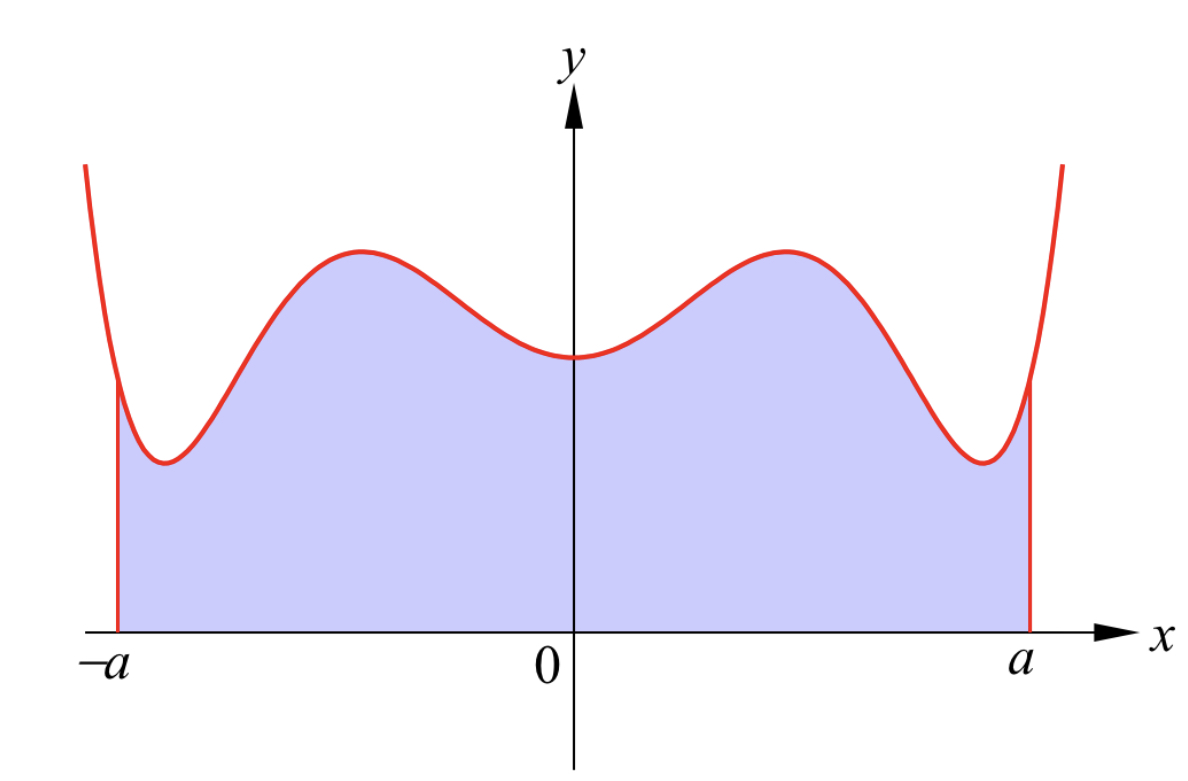
\includegraphics[scale=0.2]{Picture46.png}
\caption{An even function.\fa}\label{figure46}
\end{figure}

\begin{figure}[ht]
\centering
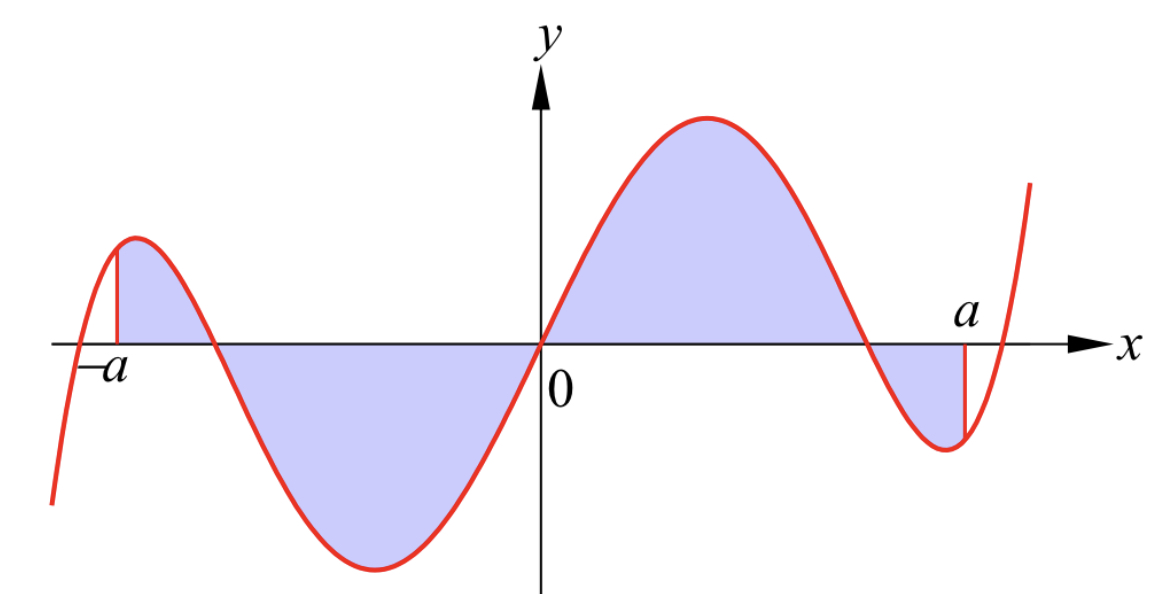
\includegraphics[scale=0.2]{Picture47.png}
\caption{An odd function.\fa}\label{figure47}
\end{figure}
\begin{example}{Area of a Circle}
 Find the area of a circle of radius $r$.

 
\begin{center}
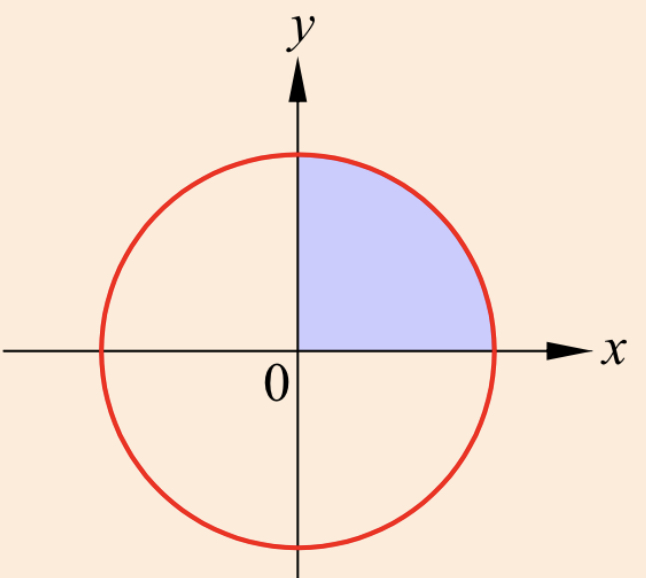
\includegraphics[scale=0.2]{Picture45.png}\end{center}
 
 
\end{example}
 
\begin{solution}{Solution}
A circle of radius $r$ with center at the origin has equation $x^2+y^2=r^2$. By symmetry, it is enough for us to find the area in the first quadrant, and then multiply by 4. The sector in the first quadrant is bounded by the curve $y=\sqrt{r^2-x^2}$, the lines $x=0$, $x=r$, and the $x$-axis.  Hence, the area of a circle of radius $r$ is
\[A=4\int_0^{r}\sqrt{r^2-x^2}dx.\]
Making a change of variables $x=r\sin\theta$, we find that 
\[\frac{dx}{d\theta}=r\cos\theta.\]When $x=0$, $\theta=0$; when $x=r$, $\theta=\pi/2$. Therefore,
\begin{align*}
A&=4\int_0^{\frac{\pi}{2}}\sqrt{r^2-r^2\sin^2\theta}\;r\cos\theta \,d\theta\\&=4r^2\int_0^{\frac{\pi}{2}}\cos^2\theta\,d\theta.\end{align*}
 Using the formula
\[\cos^2\theta=\frac{1+\cos 2\theta}{2},\]
we have
\begin{align*}A &=2r^2\int_0^{\frac{\pi}{2}}\left(1+\cos2\theta\right)d\theta \\&=2r^2\left[\theta+\frac{\sin2\theta}{2}\right]_0^{\frac{\pi}{2}} \\&=2r^2\times\frac{\pi}{2}\\&=\pi r^2.\end{align*}
\end{solution}
\subsection{Integration by Parts}

\begin{theorem}{Integration by Parts}
Let $f:[a,b]\to\mathbb{R}$ and $g:[a,b]\to\mathbb{R}$ be  functions that satisfy the following conditions:
\begin{enumerate}[(i)]
\item $f$ and $g$ are continuous on $[a,b]$;
\item $f$ and $g$ are  continuously differentiable on $(a,b)$;
\item $f'(x)$ and $g'(x)$ are bounded on $(a,b)$.
\end{enumerate}Then $fg'$ and $gf'$ are Riemann integrable on $[a,b]$, and
\[\int_a^b f(x)g'(x)dx=f(b)g(b)-f(a)g(a)-\int_a^bg(x) f'(x)dx.\]
\end{theorem}
\begin{myproof}{Proof}
Since  $f$ and $g$ are continuous on $[a,b]$, they are bounded. Since $f'(x)$ and $g'(x)$ are conitnuous and bounded on $(a,b)$, $fg'$ and $f'g$ are continuous and bounded on $(a,b)$. Therefore, $fg'$ and $gf'$ are Riemann integrable on $[a,b]$. By product rule, for any $x\in (a,b)$, 
\[(fg)'(x)=f(x)g'(x)+g(x)f'(x).\]
So $(fg)'$ is also bounded and continuous on $(a,b)$, and hence Riemann integrable on $[a,b]$. Since $fg$ is also continuous on $[a,b]$, we can apply  fundamental theorem of calculus, which gives
\[\int_a^b (fg)'(x)dx=(fg)(b)-(fg)(a).\]
Therefore,
\[\int_a^b f(x)g'(x)dx+\int_a^b g(x)f'(x)dx= f(b)g(b)-f(a)g(a).\]This proves the integration by parts formula.
\end{myproof}In a nutshell, the integration by parts formula is just the inverse of the product rule of differentiation. But it is a very useful integration technique.
\begin{highlight}{Integration by Parts}
The integration by parts formula is often expressed as
\[\int udv=uv-\int vdu.\]
In practice, we  identify which part should be $u$ and which part should be $dv$. The function $v$ is defined up to a constant.  One can verify directly that if $v$ is replaced by $v+C$, where $C$ is a constant, the right hand side of the formula is not changed. Hence, we can choose a $v$ that is most convenient.
\end{highlight}

\begin{example}{}
Let $n$ be a positive integer. Evaluate the integral
\[\int_1^e\frac{\ln x}{x^n}dx.\]

\end{example}
\begin{solution}{Solution}If $n=1$, we use integration by substitution with $u=\ln x$. Then
\[\frac{du}{dx}=\frac{1}{x}.\]
When $x=1$, $u=0$; when $x=e$, $u=1$. Therefore,
\[\int_1^e\frac{\ln x}{x}dx=\int_0^1udu=\left[\frac{u^2}{2}\right]_{0}^1=\frac{1}{2}.\]
If $n\geq 2$, we use integration by parts. Let 
\[u(x)=\ln x,\hspace{1cm}v'(x)=\frac{1}{x^{n}}.\]
Then
\[\frac{du}{dx}=\frac{1}{x},\quad v(x)=-\frac{1}{n-1}\times\frac{1}{x^{n-1}}.\]Both of $u(x)$ and $v(x)$ are continuously differentiable functions on $(0,\infty)$. 
\bs Therefore,
\begin{align*}\int_1^e\frac{\ln x}{x^n}dx&=\left[-\frac{1}{n-1}\times\frac{\ln x}{x^{n-1}}\right]_1^e+\frac{1}{n-1}\int_1^e\frac{1}{x^{n}}dx\\
&=-\frac{1}{n-1}\times\frac{1}{e^{n-1}}-\frac{1}{(n-1)^2}\left[\frac{1}{x^{n-1}}\right]_1^e\\
&=\frac{1}{(n-1)^2}-\frac{n}{(n-1)^2}\frac{1}{e^{n-1}}.
\end{align*}
\end{solution}
\begin{example}[label=230307_10]{}Let $I$ be an open interval that contains the point $x_0$, and 
let $f:I\to\mathbb{R}$ be a continuous function. Given  a positive integer $n$, define the function $F:I\to\mathbb{R}$ by
\[F(x)=\frac{1}{n!}\int_{x_0}^x(x-t)^nf(t)dt.\]
Prove that $F$ is $(n+1)$ times continuously differentiable, 
\[F(x_0)=F'(x_0)=\ldots=F^{(n)}(x_0)=0,\]
and
\[F^{(n+1)}(x)=f(x)\hspace{1cm}\text{for all}\;x\in I.\]
\end{example}
\begin{solution}
{Solution}
Define the function $g:\mathbb{R}\to\mathbb{R}$ by
\[g(x)=\int_{x_0}^xf(t)dt.\] Then $g(x_0)=0$, and 
by fundamental theorem of calculus,
\[g'(x)=f(x)\hspace{1cm}\text{for all}\;x\in I.\]

Now we prove the statement by induction on $n$. When $n=1$, 
\[F(x)=\int_{x_0}^x(x-t)f(t)dt.\]\bs
By definition, $F(x_0)=0$. 
For a fixed $x$, using integration by parts with $u(t)=x-t$ and $v'(t)=f(t)$, we find that  
\[\frac{du}{dt}=-1, \quad v(t)=g(t).\]  
It follows that
\[F(x)=\Bigl[(x-t)g(t)\Bigr]_{t=x_0}^{t=x}+\int_{x_0}^x g(t)dt=\int_{x_0}^x g(t)dt.\] Notice that $g(t)$ is continuously differentiable, and hence it is continuous. By fundamental theorem of calculus, 
\[F'(x)=g(x)\hspace{1cm}\text{for all}\;x\in I.\]
Therefore, $F'(x_0)=g(x_0)=0$, and 
\[F''(x)=g'(x)=f(x)\hspace{1cm}\text{for all}\;x\in I.\]
This proves that $F(x)$ is twice continuously differentiable. Since we have also shown that $F(x_0)=F'(x_0)=0$, and $F''(x)=f(x)$ for all $x\in I$.
 the statement is true when $n=1$.

Assume that we have proved the statement when $n=k-1$, where $k\geq 2$. When $n=k$, 
\[F(x)=\frac{1}{k!}\int_{x_0}^x(x-t)^kf(t)dt.\]
  For a fixed $x$, using integration by parts with $u(t)=(x-t)^k$ and $v'(t)=f(t)$, we find that 
\[\frac{du}{dt}=-k(x-t)^{k-1}, \quad v(t)=g(t).\] 
It follows that
\begin{align*}F(x)&=\frac{1}{k!}\left[(x-t)^kg(t)\right]_{t=x_0}^{t=x}+\frac{1}{(k-1)!}\int_{x_0}^x (x-t)^{k-1}g(t)dt\\&=\frac{1}{(k-1)!}\int_{x_0}^x (x-t)^{k-1}g(t)dt.\end{align*}
By inductive hypothesis, the function
$F(x)$ satisfies 
\[F(x_0)=F'(x_0)=\cdots=F^{(k-1)}(x_0)=0,\]\bs
and
\[F^{(k)}(x)=g(x)\hspace{1cm}\text{for all}\;x\in I.\] 
The latter implies that $F^{(k)}(x_0)=g(x_0)=0$, and $F(x)$ is $(k+1)$ times differentiable, with
\[F^{(k+1)}(x)=g'(x)=f(x) \] a continuous function. Therefore, when $n=k+1$, the statement also holds. 


By principle of mathematical induction, the statement is true for all positive integers $n$.
\end{solution}

\vp
\noindent
{\bf \large Exercises  \thesection}
\setcounter{myquestion}{1}
\atc
\begin{question}{\themyquestion}Let $f:[a,b]\to\mathbb{R}$ be a bounded function that is Riemann integrable.
Show that for any real number $c$,
\[\int_a^bf(x)dx=\int_{a+c}^{b+c}f(x-c)dx.\]
\end{question}
\begin{question}{\themyquestion}
Explain why  
\[\int_{-1}^1 (x+1)e^{-x^2}dx=2\int_0^1e^{-x^2}dx.\]
\end{question}
 
\atc
\begin{question}{\themyquestion}
 Let $a$ be a positive number. Assume that the functions $f:[0,a]\to\mathbb{R}$ and $g:[0,a]\to\mathbb{R}$ are bounded and piecewise continuous, prove that
\[\int_0^af(x)g(a-x)dx=\int_0^af(a-x)g(x)dx.\]
\end{question}
 \atc
\begin{question}[label=ex230225_1]{\themyquestion}
 Let $m$ and $n$ be nonnegative integers. Show that
\[\int_0^1x^m(1-x)^ndx=\frac{m!\,n!}{(m+n+1)!}.\]
\end{question}

 \atc
\begin{question}{\themyquestion}
 Let $f:[a,b]\to\mathbb{R}$ be a continuous and strictly increasing function which maps the interval $[a,b]$ bijectively onto the interval $[c,d]$, where $c=f(a)$, and $d=f(b)$. Denote by $g:[c,d]\to\mathbb{R}$  the inverse function of $f$. Notice that  $f:[a,b]\to\mathbb{R}$ and $g:[c,d]\to\mathbb{R}$ are Riemann integrable. This question is regarding the proof of the formula
\begin{equation}\label{eq230224_1}\int_a^bf(x)dx=bf(b)-af(a)-\int_c^dg(x)dx.\end{equation}
 \begin{enumerate}[(a)]
\item If $a>0$ and $c>0$,  draw a figure to illustrate  the formula.
\item If $f$ is continuously differentiable on $(a,b)$,  
use integration by substitution with $u=g(x)$ to prove the formula \eqref{eq230224_1}.

 \item  Let $P_n=\{x_i\}_{i=0}^n$ be the regular partition of the interval $[a,b]$ into $n$ intervals. For $0\leq i\leq n$, let $y_i=f(x_i)$. Then $\widetilde{P}_n=\{y_i\}_{i=0}^n$ is a partition of $[c,d]$. 
\begin{enumerate}[(i)]
\item
Show that \[\sum_{i=1}^n f(x_{i-1})(x_i-x_{i-1})+\sum_{i=1}^n g(y_i)(y_i-y_{i-1})=bf(b)-af(a).\]
\item Show that $\di\lim_{n\to\infty}|P_n|=0$ and  $\di\lim_{n\to\infty}|\widetilde{P}_n|=0$. You might want to use uniform continuity.
\item Use part (i) and part (ii) to prove the formula
 \eqref{eq230224_1}.
\end{enumerate}
\end{enumerate}
\end{question}
\vp



\section{Improper Integrals}\label{sec4.6}
In this section, we want to discuss Riemann integrals for functions $f:I\to\mathbb{R}$ defined on an interval $I$, where either $I$ is not bounded, or $f$ is not bounded on $I$, or both. 

\begin{definition}{Improper Integral}
Let $I$ be an interval and let  $f:I\to\mathbb{R}$ be a function defined on $I$.  An integral of the form
\[\int_If\] is an improper integral if either $f$ is not bounded on $I$, or $I$ is an unbounded interval.
\end{definition}
This is not a rigorous definition. We will only be interested in the case where we can make sense of $\di\int_If$.

As an example,  Theorem  \ref{thm230222_13} says that there exists a differentiable function $g:(-1,1)\to\mathbb{R}$ satifying
\[g'(x)=\frac{1}{\sqrt{1-x^2}},\hspace{1cm}g(0)=0.\]It is given by
\[g(x)=\int_0^x\frac{du}{\sqrt{1-u^2}}du.\]
Notice that the function $\di f(u)=\di\frac{1}{\sqrt{1-u^2}}$ is bounded and continuous on the interval $[0,x]$ if $0< x<1$, and on $[x,0]$ if $-1<x<0$. Therefore, $g(x)$ is a well-defined Riemann integral when $-1<x<1$. We are interested to extend the definition of $g(x)$ to $x= 1$ and $x=-1$. But $f$ is not bounded on $(-1,1)$, so we cannot define the Riemann integral of $f$ on $[0, 1]$ or $[-1,0]$.  Our studies on the function $\sin x$ shows that $g(x)=\sin^{-1}x$ when $x\in(-1,1)$. Thus,
\[\lim_{x\to 1^-}g(x)=\sin^{-1}1=\frac{\pi}{2},\hspace{1cm}\lim_{x\to -1^+}g(x)=\sin^{-1}(-1)=-\frac{\pi}{2}.\]
Hence, it is reasonable to say that the improper integrals 
\[\int_0^{1}\frac{1}{\sqrt{1-u^2}}du\quad\text{and}\quad \int_0^{-1}\frac{1}{\sqrt{1-u^2}}du\] have values
\[\lim_{x\to 1^-}\int_0^{x}\frac{1}{\sqrt{1-u^2}}du=\frac{\pi}{2}\quad\text{and}\quad\lim_{x\to -1^+}\int_0^{x}\frac{1}{\sqrt{1-u^2}}du=-\frac{\pi}{2}\]respectively. This is how we are going to make sense of improper integrals.  
\begin{definition}
{Improper Integrals of Unbounded Functions}
\begin{enumerate}[1.]
\item
If the function $f:(a, b]\to\mathbb{R}$ is not bounded, but it is bounded and Riemann integrable on any interval $[c,b]$ with $a<c<b$, then we say that the improper integral $\di\int_a^bf(x)dx$ is convergent if  the limit
\[\lim_{c\to a^+}\int_c^bf(x)dx\]   exists. Otherwise, we say that the improper integral   is divergent. When the improper integral is convergent, we define its value as
\[ \int_a^bf(x)dx=\lim_{c\to a^+}\int_c^bf(x)dx.\] 
\item If the function $f:[a, b)\to\mathbb{R}$ is not bounded, but it is bounded and Riemann integrable on any interval $[a,c]$ with $a<c<b$, then we say that the improper integral $\di\int_a^bf(x)dx$ is convergent if  the limit
\[\lim_{c\to b^-}\int_a^cf(x)dx\]   exists. Otherwise, we say that the improper integral   is divergent. When the improper integral is convergent, we define its value as
\[ \int_a^bf(x)dx=\lim_{c\to b^-}\int_a^cf(x)dx.\] 

\end{enumerate}
\end{definition}

\begin{highlight}{Improper Integrals of Unbounded Functions}
Putting in another way, if the function $f:(a, b]\to\mathbb{R}$ is not bounded, but  it is bounded and Riemann integrable on any  intervals $[x,b]$  when $a<x<b$, we define the function $F:(a,b]\to\mathbb{R}$ by
\[F(x)=\int_x^{b}f(u)du.\]
Then $F$ is a continuous function. We say that the improper integral $\di\int_a^{b}f(x)dx$ is convergent if and only if 
\[\lim_{x\to a^+}F(x)\] exists.
Similarly, for a function $f:[a,b)\to\mathbb{R}$ that is not bounded, but is bounded and Riemann integral on any  intervals $[a,x]$ when $a<x<b$,  we say that the improper integral $\di\int_{a}^bf(x)dx$ is convergent if and only if the continuous function $F:[a,b)\to\mathbb{R}$ defined by
\[F(x)=\int_{a}^x f(u)du\] has a limit when $x\to b^-$.
\end{highlight}
\begin{example}{}
$\di\int_0^1\frac{1}{\sqrt{1-x^2}}dx$ is an improper integral as the function $f:[0,1)\to\mathbb{R}$, $f(x)=\di \frac{1}{\sqrt{1-x^2}}$ is not bounded. We have seen that this improper integral is convergent and has value $\di \frac{\pi}{2}$.
\end{example}

\begin{example}[label=ex230227_10]{}
Let $p$ be a positive number. Determine those values of $p$ for which the improper integral $\di\int_0^1\frac{1}{x^p}dx$ is convergent. Find the value of the improper integral when it is convergent.
\end{example}
\begin{solution}
{Solution}
For $p>0$, define the function $F:(0, 1]\to\mathbb{R}$ by 
\[F(x)=\int_x^1\frac{1}{u^p}du.\]Then
\begin{align*}
F(x)=\begin{cases}-\ln x,\quad &\text{if}\; p=1,\\
\di \frac{1-x^{1-p}}{1-p},\quad &\text{if}\; p\neq 1.\end{cases}
\end{align*} From this, we see that
$\di \lim_{x\to 0^+}F(x)$ exists if and only if $0<p<1$. Hence, the improper integral  $\di\int_0^1\frac{1}{x^p}dx$ is convergent if and only if $0<p<1$. In this case, 
\[\int_0^1\frac{1}{x^p}dx=\frac{1}{1-p},\quad 0<p<1.\]
\end{solution}
When $r\geq 0$, the integral $\di\int_0^1 x^rdx$ is just an ordinary integral. However, we will sometimes abuse terminology and say that the integral $\di\int_0^1x^rdx$ is convergent if and only if $r>-1$. 
\begin{highlight}{}
If $c$ is a point in $(a,b)$ and we have a function $f:[a,b]\setminus\{c\}\to\mathbb{R}$  that is not bounded, we will define the improper integral $\di\int_a^bf(x)dx$ as 
\[\int_a^cf(x)dx+\int_c^bf(x)dx.\]
We say that  the improper integral $\di\int_a^bf(x)dx$ is convergent provided that both improper integrals $\di \int_a^cf(x)dx$ and $\di \int_c^bf(x)dx$ are convergent. 
\end{highlight}
Next we consider improper integrals defined on unbounded intervals.
\begin{definition}{Improper integrals on Unbounded Intervals}
\begin{enumerate}[1.]
\item
If $f:[a,\infty)\to\mathbb{R}$ is a  function that is bounded and Riemann integrable on any bounded intervals $[a, b]$, we say that the improper integral $\di\int_a^{\infty}f(x)dx$ is convergent if the limit
\[\lim_{b\to\infty}\int_a^{b}f(x)dx\] exists. Otherwise, we say that the improper integral is divergent.
If the improper integral is convergent, we define its value as  
\[\int_a^{\infty}f(x)dx=\lim_{b\to\infty}\int_a^{b}f(x)dx.\]
\item
If $f:(-\infty,b]\to\mathbb{R}$ is a   function that is bounded and Riemann integrable on any bounded intervals $[a, b]$, we say that the improper integral $\di\int^b_{-\infty}f(x)dx$ is convergent if the limit
\[\lim_{a\to-\infty}\int_a^{b}f(x)dx\] exists. Otherwise, we say that the improper integral is divergent.
If the improper integral is convergent, we define its value as   
\[\int^b_{-\infty}f(x)dx=\lim_{a\to-\infty}\int_a^{b}f(x)dx.\]
\item If $f:\mathbb{R}\to\mathbb{R}$ is a function that is bounded and Riemann integrable on any bounded intervals $[a,b]$, we say that the improper integral $\di\int_{-\infty}^{\infty}f(x)dx$ is convergent if and only if for any  real number $c$, both the improper integrals 
\[\int_{-\infty}^{c}f(x)dx\hspace{1cm}\text{and}\hspace{1cm}\int_{c}^{\infty}f(x)dx\] are convergent. In such a case, we define the improper integral as
\begin{equation}\label{eq230224_2}\int_{-\infty}^{\infty}f(x)dx=\int_{-\infty}^cf(x)dx+\int_c^{\infty}f(x)dx.\end{equation}
\end{enumerate}
\end{definition}
\begin{remark}{}
 To make the integral $\di\int_{-\infty}^{\infty}f(x)dx$ well defined when it is convergent, we need to check that the right hand side of \eqref{eq230224_2} does not depend on the point $c$. 
In fact, we can show that if there is a real number $c_0$ so that both the improper integrals 
\[\int_{-\infty}^{c_0}f(x)dx\hspace{1cm}\text{and}\hspace{1cm}\int_{c_0}^{\infty}f(x)dx\] are convergent,  then for any other values of $c$, \[\int_{-\infty}^{c}f(x)dx\hspace{1cm}\text{and}\hspace{1cm}\int_{c}^{\infty}f(x)dx\] are convergent. This is just due to additivity, which says that
\begin{align*}\int_a^cf(x)dx&=\int_a^{c_0}f(x)dx+\int_{c_0}^cf(x)dx,\\
\int_c^bf(x)dx&=\int_{c}^{c_0}f(x)dx+\int_{c_0}^bf(x)dx.\end{align*}
Thus, $\di\lim_{a\to-\infty}\int_a^cf(x)dx$ exists if and only if $\di\lim_{a\to-\infty}\int_a^{c_0}f(x)dx$ exists, and 
$\di\lim_{b\to\infty}\int_c^bf(x)dx$ exists if and only if 
$\di\lim_{b\to \infty}\int_{c_0}^{b}f(x)dx$ exists. Moreover,
 \begin{align*}\lim_{a\to-\infty}\int_a^cf(x)dx&=\lim_{a\to-\infty}\int_a^{c_0}f(x)dx+\int_{c_0}^cf(x)dx,\\
\lim_{b\to\infty}\int_c^bf(x)dx&=\int_{c}^{c_0}f(x)dx+\lim_{b\to\infty}\int_{c_0}^bf(x)dx.\end{align*}
Since $\di \int_{c_0}^cf(x)dx=-\int_{c}^{c_0}f(x)dx$, we find that
\[\int_{-\infty}^{c_0}f(x)dx+\int_{c_0}^{\infty}f(x)dx=\int_{-\infty}^{c}f(x)dx+\int_{c}^{\infty}f(x)dx.\]
\end{remark}
\begin{highlight}{Improper Integrals on Unbounded Intervals}
Putting in another way, if $f:[a,\infty)\to\mathbb{R}$ is a function that is bounded and Riemann integrable on any bounded intervals, we define the function $F:[a,\infty)\to\mathbb{R}$ by
\[F(x)=\int_a^{x}f(u)du.\]
Then $F$ is a continuous function. We say that the improper integral $\di\int_a^{\infty}f(x)dx$ is convergent if and only if the limit
\[\lim_{x\to\infty}F(x)\] exists.
Similarly, for a function $f:(-\infty, b]\to\mathbb{R}$ that is bounded and Riemann integrable on any bounded intervals $[a,b]$, we say that the improper integral $\di\int_{-\infty}^bf(x)dx$ is convergent if and only if the continuous function $F:(-\infty, b]\to\mathbb{R}$ defined by
\[F(x)=\int_{x}^b f(u)du\] has a limit when $x\to-\infty$.
\end{highlight}

\begin{example}{}
Let $p$ be any real number. Determine those values of $p$ for which the improper integral $\di\int_1^{\infty}\frac{1}{x^p}dx$ is convergent. Find the value of the improper integral when it is convergent.
\end{example}
\begin{solution}{Solution}
For a fixed real number $p$, define the function $F:[1,\infty)\to\mathbb{R}$ by
\[F(x)=\int_1^x\frac{1}{u^p}dx.\]\bs
Then
\begin{align*}
F(x)=\begin{cases} \ln x,\quad &\text{if}\; p=1,\\
\di\frac{x^{1-p}-1}{1-p},\quad &\text{if}\;p\neq 1.\end{cases}
\end{align*}From this, we see that the limit $\di\lim_{x\to\infty}F(x)$ exists if and only if $p>1$. Hence, the improper integral  $\di\int_1^{\infty}\frac{1}{x^p}dx$ is convergent if and only if $p>1$, and
\[  \int_1^{\infty}\frac{1}{x^p}dx=\frac{1}{p-1},\quad p>1.\]
\end{solution}

\begin{example}{}
Determine whether the improper integral  is convergent. If yes, find the value of the integral.
\begin{enumerate}[(a)]
\item 
$\di \int_0^{\infty}\frac{1}{1+x^2}dx$
\item $\di \int_{-\infty}^0e^{x}dx$
\item $\di\int_{-\infty}^{\infty}\frac{x}{x^2+1}dx$
\end{enumerate}
\end{example}
\begin{solution}{Solution}
\begin{enumerate}[(a)]
\item
Since $\di\frac{d}{dx}\tan^{-1}x=\frac{1}{1+x^2}$, we find that
\[\int_0^b \frac{1}{1+x^2}dx=\tan^{-1}b-\tan^{-1}0=\tan^{-1}b.\]
Since
\[\lim_{b\to\infty}\tan^{-1}b=\frac{\pi}{2},\]the improper integral $\di \int_0^{\infty}\frac{1}{1+x^2}dx$ is convergent and its value is \end{enumerate}\bs\begin{enumerate}[(a)]\item[]
\[ \int_0^{\infty}\frac{1}{1+x^2}dx=\lim_{b\to\infty} \int_0^b \frac{1}{1+x^2}dx =\lim_{b\to\infty} \tan^{-1}b=\frac{\pi}{2}.\]
\item[(b)] Since $e^a\to 0$ as $a\to-\infty$, we have
\[ \int_{-\infty}^0e^{x}dx=\lim_{a\to -\infty}\int_a^{0}e^xdx=\lim_{a\to-\infty}\left(1-e^a\right)=1.\]The improper integral  $\di \int_{-\infty}^0e^{x}dx$ is convergent and is equal to 1.
\item[(c)] Here, we consider the improper integrals
\[\int_{-\infty}^0\frac{x}{x^2+1}dx\hspace{1cm}\text{and}\hspace{1cm}\int_0^{\infty} \frac{x}{x^2+1}dx.\]
Since
\[\frac{d}{dx}\ln(1+x^2)=\frac{2x}{1+x^2},\]we find that
\[\int_0^b\frac{x}{1+x^2}dx=\frac{1}{2}\ln(1+b^2).\]
But \[\lim_{b\to\infty}\ln(1+b^2)=\infty.\]
Hence,
 the improper integral $\di\int^{\infty}_0\frac{x}{x^2+1}dx$ is divergent. So, the improper integral  $\di\int_{-\infty}^{\infty}\frac{x}{x^2+1}dx$ is also divergent.
\end{enumerate}
\end{solution}
One is tempted to  
define the improper integral  
$\di\int_{-\infty}^{\infty}f(x)dx$  as
\[\lim_{a\to \infty}\int_{-a}^af(x)dx\] if it exists. For part (c) in the example above, $\di f(x)=\frac{x}{1+x^2}$ is an odd function. Thus, $\di \int_{-a}^a\frac{x}{1+x^2}dx=0$ for any $a$, and so
\[\lim_{a\to \infty}\int_{-a}^a\frac{x}{1+x^2}dx=0.\]
In fact, if $f:\mathbb{R}\to\mathbb{R}$ is an odd function, then we always have
\[\lim_{a\to \infty}\int_{-a}^af(x)dx=0.\]If we use   the limit \[\lim_{a\to \infty}\int_{-a}^af(x)dx\] as a definition for the improper integral $\di\int_{-\infty}^{\infty}f(x)dx$, it will lead to  undesirable results, such as that the integral $\di \int_{-\infty}^{\infty} xdx$ is convergent. Nevertheless,  the limit \[\lim_{a\to \infty}\int_{-a}^af(x)dx,\] if it exists, has some applications. It is called the Cauchy principal value of $\di\int_{-\infty}^{\infty}f(x)dx$.


\begin{definition}{Cauchy Principal Value}
If $f:\mathbb{R}\to\mathbb{R}$ is a function that is bounded and Riemann integrable on any symmetric bounded intervals $[-a,a]$, the Cauchy principal value of the improper integral $\di\int_{-\infty}^{\infty}f(x)dx$, denoted by $\text{P.V.}\, \di\int_{-\infty}^{\infty}f(x)dx$, is defined as
\[\text{P.V.}\,\int_{-\infty}^{\infty}f(x)dx=\lim_{a\to \infty}\int_{-a}^af(x)dx,\]
if the limit exists.
\end{definition}  
Thus, we find that if $f:\mathbb{R}\to\mathbb{R}$ is an odd function, then $\di\text{P.V.}\,\int_{-\infty}^{\infty}f(x)dx=0$. It is also easy to prove the following.

\begin{proposition}[label=230224_10]{} If the improper integral  $\di\int_{-\infty}^{\infty}f(x)dx$ is convergent, then 
its Cauchy principal value exists, and is equal to the improper integral. Namely, 
\[\text{P.V.}\,  \int_{-\infty}^{\infty}f(x)dx=  \int_{-\infty}^{\infty}f(x)dx.\]
\end{proposition}
\begin{myproof}{Proof}
If  the improper integral $\di \int_{-\infty}^{\infty}f(x)dx$ is convergent, then  the limits
\[\lim_{  c\to-\infty } \int_c^0f(x)dx\quad\text{and}\quad\lim_{b\to\infty}\int_0^bf(x)dx\]exists and
\[ \int_{-\infty}^{\infty}f(x)dx=\lim_{  c\to-\infty } \int_c^0f(x)dx+\lim_{b\to\infty}\int_0^bf(x)dx. \] This implies that 
\[ \lim_{a\to \infty} \int_{-a}^af(x)dx=
\lim_{a\to\infty}\int_{-a}^0f(x)dx+\lim_{a\to\infty}\int_0^af(x)dx=\int_{-\infty}^{\infty}f(x)dx.\] 
\end{myproof}


Consider the integral
\begin{equation}\label{eq230224_4}\int_0^{\infty}\frac{1}{\sqrt{x}(x+1)}dx.\end{equation}
The function $f:(0,\infty)\to\mathbb{R}$,
\[f(x)=\frac{1}{\sqrt{x}(x+1)}\] is not bounded on any interval $(0, b]$ when $b>0$. Hence, the integral is an improper integral of an unbounded function defined on an unbounded interval. Using the same principle, we will say that it is convergent if and only if for any $c>0$,  the improper integrals 
\[\int_0^cf(x)dx\hspace{1cm}\text{and}\hspace{1cm}\int_c^{\infty}f(x)dx\] are convergent. 

Another natural question to ask is whether one can determine whether an improper integral is convergent without explicitly computing the integral. There are some partial solutions to this. 

\begin{highlight}
{}If $J$ is an interval that is contained in the interval $I$, and the integral $\di\int_J f(x)dx$ is divergent, then the integral $\di\int_I f(x)dx$ is divergent. 
\end{highlight}
For instance, the integral $\di\int_0^{\infty}f(x)dx$ is divergent  if  the integral $\di\int_1^{\infty}f(x)dx$ is divergent.

The next proposition says that linear combination  of convergent integrals must be convergent.
\begin{proposition}{Linearity}
Let $I$ be an interval. If the improper integrals $\di\int_If(x)dx$ and $\di\int_Ig(x)dx$ are convergent, then for any constants $\alpha$ and $\beta$, the improper integral $\di\int_I(\alpha f+\beta g)$ is also convergent, and
\[\int_I(\alpha f+\beta g)=\alpha\int_If+\beta\int_I g.\]
\end{proposition}This follows easily from limit laws.
Now we want to prove some comparison theorems for improper integrals. We start with integrals of nonnegative functions. If a function $f $ is nonpositive, one just consider the function $-f$, which is then nonnegative. 
 
\begin{lemma}[label=230224_5]{} Let $I$ be an interval. Given that $f:I\to\mathbb{R}$  is a nonnegative function that is bounded and Riemann integrable on any closed and bounded intervals that are contained in $I$. Fixed $x_0$ in $I$ and define the function $F:I\to\mathbb{R}$ by
\[F(x)=\int_{x_0}^xf(u)du.\]
\begin{enumerate}[1.]
\item If $I=(a, b]$ or $I=(-\infty,b]$, then the integral $\di\int_I f(x)dx$ is convergent if and only if the function $F(x)$ is bounded below. 
\item If $I=[a,b)$ or $I=[a,\infty)$, then the integral $\di\int_If(x)dx$ is convergent if and only if the function $F(x)$ is bounded above. 
 \end{enumerate}
\end{lemma}

\begin{myproof}{Proof}
Notice that since $f(u)\geq 0$ for all $u\in I$, for any $x_1$ and $x_2$ in $I$, if $x_1<x_2$, then 
\[F(x_2)-F(x_1)=\int_{x_1}^{x_2}f(u)du\geq 0.\]
This implies that $F:I\to\mathbb{R}$ is an increasing function. \begin{enumerate}[1.]
\item If $I=(a,b]$ or $I=(-\infty, b]$, the limit $\di\lim_{x\to a^+}F(x)$ or the limit $\di\lim_{x\to-\infty}F(x)$ exists if and only if $F(x)$ is bounded below. \item If $I=[a, b)$ or $I=[a, \infty)$, the  limit $\di\lim_{x\to b^-}F(x)$ or the limit $\di\lim_{x\to \infty}F(x)$ exists if and only if $F(x)$ is bounded above. \end{enumerate}
\end{myproof}

In Proposition \ref{230224_10}, we have stated that if the improper integral $\di\int_{-\infty}^{\infty}f(x)dx$ is convergent, then the Cauchy principal value $\di \text{P.V.} \di\int_{-\infty}^{\infty}f(x)dx$  exists. The converse is true if the function $f:\mathbb{R}\to\mathbb{R}$ is nonnegative.
\begin{theorem}{}
Let $f:\mathbb{R}\to\mathbb{R}$ be a nonnegative function that is bounded and Riemann integrable on any closed and bounded intervals. The improper integral $\di\int_{-\infty}^{\infty}f(x)dx$ is convergent if and only if the Cauchy principal value $\di \text{P.V.} \di\int_{-\infty}^{\infty}f(x)dx$  exists. Moreover, 
\[\int_{-\infty}^{\infty}f(x)dx=\text{P.V.} \di\int_{-\infty}^{\infty}f(x)dx.\]

\end{theorem}
\begin{myproof}{Proof}We just need to show that if the Cauchy principal value $\di \text{P.V.} \di\int_{-\infty}^{\infty}f(x)dx$  exists, then the improper integral $\di\int_{-\infty}^{\infty}f(x)dx$ is convergent.\bp
Assume that the Cauchy principal value $\di \text{P.V.} \di\int_{-\infty}^{\infty}f(x)dx$  exists and is equal to $I$. As in the proof of Lemma \ref{230224_6}, the function 
\[F(x)=\int_{0}^xf(u)du\]  is an increasing function.  For any real numbers $b$ and $c$ with $b\leq c$, there is a positive number $a$ such that
\[-a\leq b\leq c\leq a.\]Hence,
\[F(c) -F(b)=\int_b^cf(x)dx\leq\int_{-a}^af(x)dx \leq I.\]
This proves that $-I\leq F(x)\leq I$ for all $x\in \mathbb{R}$. In other words, the function $F:\mathbb{R}\to\mathbb{R}$ is bounded. Therefore, the improper integrals $\di\int_0^{\infty}f(x)dx$ and  $\di\int_{-\infty}^0f(x)dx$ are convergent, and so the improper integral $\di\int_{-\infty}^{\infty}f(x)dx$ is convergent.
\end{myproof}

Now, we can present the comparison theorem for improper integrals.
\begin{theorem}[label=230224_6]{Comparison Theorem}
 Let $I$ be an interval. Given that $f:I\to\mathbb{R}$ and $g:I\to\mathbb{R}$ are nonnegative functions that are bounded and Riemann integrable on any closed and bounded intervals that are contained in $I$. Assume that
\[0\leq f(x)\leq g(x)\hspace{1cm}\text{for all}\;x\in I.\]
\begin{enumerate}[1.]\item If the integral $\di\int_Ig(x)dx$ is convergent, then the integral $\di\int_I f(x)dx$ is convergent. 
\item If the integral $\di\int_If(x)dx$ is divergent, then the integral $\di\int_I g(x)dx$ is divergent. 
\end{enumerate}
\end{theorem}
\begin{myproof}{Proof}Notice that the second statement is the contrapositive of the first statement. Hence, we only need to prove the first statement. 
Fixed $x_0$ in the interval $I$, and define
\[F(x)=\int_{x_0}^x f(u)du,\hspace{1cm} G(x)=\int_{x_0}^x g(u)du.\]
If $x>x_0$,
\[0\leq F(x)\leq G(x).\]
Therefore, $G$ is bounded above implies $F$ is bounded above.
  If $x<x_0$,
\[F(x)=-\int_{x}^{x_0}f(u)du,\hspace{1cm}G(x)=-\int_{x}^{x_0}g(u)du.\] Since
\[0\leq \int_{x}^{x_0}f(u)du\leq \int_{x}^{x_0}g(u)du,\] we find that
\[0\geq F(x)\geq G(x).\]  Therefore, $G$ is bounded below implies that $F$ is bounded below. The assertions about the convergence of the integrals then follow  from Lemma \ref{230224_5}.
\end{myproof}
\begin{example}
{} We can show that the integral $\di\int_0^{\infty}\frac{x}{x^2+1}dx$ is divergent without explicitly computing the integral. Notice that for $x\geq 1$,
\[0\leq \frac{1}{2x}\leq\frac{x}{x^2+1}.\]
Since the integral $\di\int_1^{\infty}\frac{1}{x}dx$ is divergent, the integral $\di \int_1^{\infty}\frac{x}{x^2+1}dx$ is also divergent. Hence,  the integral $\di\int_0^{\infty}\frac{x}{x^2+1}dx$ is divergent.
\end{example}
  \begin{example}{}
Determine whether the improper integral $\di\int_0^{\infty}\frac{1}{\sqrt{x}(x+1)}dx$ is convergent.
\end{example}
\begin{solution}{Solution}
We determine  the convergence of the two improper integrals
\[\int_0^1\frac{1}{\sqrt{x}(x+1)}dx\hspace{1cm}\text{and}\hspace{1cm}\int_1^{\infty}\frac{1}{\sqrt{x}(x+1)}dx\] separately.
For $0<x\leq 1$,
\[0\leq \frac{1}{\sqrt{x}(x+1)} \leq \frac{1}{\sqrt{x}}.\] Since the integral $\di\int_0^1\frac{1}{\sqrt{x}}dx$ is convergent, the integral $\di  \int_0^1\frac{1}{\sqrt{x}(x+1)} dx$ is convergent. 
For $x\geq 1$,
\[0\leq \frac{1}{\sqrt{x}(x+1)} \leq \frac{1}{x\sqrt{x}}=\frac{1}{x^{3/2}}.\]   Since the integral $\di\int_1^{\infty}\frac{1}{x^{3/2}}dx$ is convergent, the integral $\di\int_1^{\infty}  \frac{1}{\sqrt{x}(x+1)} dx$ is convergent. From these, we conclude that the integral  $\di \int_0^{\infty}\frac{1}{\sqrt{x}(x+1)}dx$ is convergent.
\end{solution}

Since the integral $\di\int_0^1x^{-p}dx$ is convergent when $p<1$, while the integral $\di\int_1^{\infty}x^{-p}dx$ is convergent if $p>1$, $\di\int_0^{\infty}x^{-p}dx$ is not convergent for any values of $p$. Hence, to determine the convergence of the integral in the example above, we need to split the integral into two parts and compare to different $g(x)=x^{-p}$. For $x\to 0^+$, we ignore the part $1/(x+1)$ which has a finite limit. For $x\to \infty$, the leading term of $1/(x+1)$ is $1/x$. This is how we identify the correct values of $p$ to compare to.



 Theorem \ref{230224_6}  provides a useful strategy to determine the convergence of an integral in the case that the function is nonnegative. For a function that can take  both positive and negative values, we need other strategies.
 
\begin{theorem}[label=230224_8]{} Let $I$ be an interval.
Assume that $f:I\to\mathbb{R}$ is a function that is bounded and Riemann integrable on any closed and bounded intervals that are contained in $I$. If the improper integral $\di\int_I|f(x)|dx$ is convergent, then the improper integral $\di\int_If(x)dx$ is convergent.
\end{theorem}This theorem can be interpreted as absolute convergence implies convergence.
\begin{myproof}{Proof}
 Define the functions $f_+:I\to\mathbb{R}$ and $f_-:I\to\mathbb{R}$ by
\[f_+(x)=\max\{f(x), 0\},\hspace{1cm}f_-(x)=\max\{-f(x),0\}.\]
In other words,  \[f_+(x)=\begin{cases} f(x),\quad &\text{if}\; f(x)\geq 0,\\0,\quad &\text{if}\;f(x)<0,\end{cases}\]
\[f_-(x)=\begin{cases} -f(x),\quad &\text{if}\; f(x)\leq 0,\\0,\quad &\text{if}\;f(x)>0.\end{cases}\]  Notice that $f_+$ and $f_-$ are nonnegative functions, and
\[f(x)=f_+(x)-f_-(x),\hspace{1cm}|f(x)|=f_+(x)+f_-(x).\]
The second equality implies that
\[0\leq f_+(x)\leq |f(x)|,\hspace{1cm}0\leq f_-(x)\leq |f(x)|\hspace{1cm}\text{for all}\;x\in I.\]Theorem \ref{230221_15} says that the function $|f|:I\to\mathbb{R}$ is Riemann integrable on any closed and bounded intervals that are contained in $I$. \bp Question \ref{ex230224_7} says that the functions $f+:I\to\mathbb{R}$ and $f_-:I\to\mathbb{R}$ are also Riemann integrable on any closed and bounded intervals that are contained in $I$.  By Theorem  \ref{230224_6}, the improper integrals $\di \int_If_+(x)dx$ and $\di \int_If_-(x)dx$ are convergent. By linearity, the improper integral $\di\int_I f(x)dx$ is also convergent.

\end{myproof}

Combining Theorem \ref{230224_6} and Theorem \ref{230224_8}, we have the following.
\begin{theorem}[label=230224_9]{General Comparison Theorem}
 Let $I$ be an interval. Given that $f:I\to\mathbb{R}$ and $g:I\to\mathbb{R}$ are  functions that are bounded and Riemann integrable on any closed and bounded  intervals that are contained in $I$. If
\[|f(x)|\leq g(x)\hspace{1cm}\text{for all}\;x\in I,\]
and the integral $\di\int_Ig(x)dx$ is convergent, then the integral $\di\int_I f(x)dx$ is convergent. 
\end{theorem}
 

\begin{example}
{}Show that the improper integral $\di\int_1^{\infty}\frac{\sin x}{x^2}dx$ is convergent. 
\end{example}
\begin{solution}{Solution}
For any $x\geq 1$,
\[\left|\frac{\sin x}{x^2}\right|\leq\frac{1}{x^2}.\]
Since the integral $\di\int_1^{\infty}\frac{1}{x^2}dx$ is convergent, the integral  $\di\int_1^{\infty}\frac{\sin x}{x^2}dx$ is convergent. 
\end{solution}

There are some important special functions in mathematics and physics which are defined in terms of improper integrals. One such function is the gamma function, which students have probably seen in probability theory. In fact, gamma function is ubiquitous in mathematics. 

\begin{example}{}
Let $s$ be a real number. Show that the improper integral $\di\int_0^{\infty}t^{s-1}e^{-t}dt$ is convergent if and only if $s>0$.
\end{example}
\begin{solution}{Solution}
We split the integral into the two integrals $\di\int_0^{1}t^{s-1}e^{-t}dt$ and $\di\int_1^{\infty}t^{s-1}e^{-t}dt$. Notice that
\[0\leq t^{s-1}e^{-1}\leq t^{s-1}e^{-t}\leq t^{s-1}\hspace{1cm}\text{for all}\; t\in (0,1].\]
Since $\di\int_0^1t^{s-1}dt$ is convergent if and only if $s>0$, $\di\int_0^1 t^{s-1}e^{-t}dt$ is convergent if and only if $s>0$. For the integral $\di \int_1^{\infty}t^{s-1}e^{-t}dt$, notice that
\[\lim_{t\to \infty}t^{s-1}e^{-t/2}=\lim_{t\to\infty} \frac{t^{s-1}}{e^{t/2}}=0.\]
Therefore, there is a number $t_0>1$ such that for all $t\geq t_0$, $t^{s-1}e^{-t/2}\leq 1$. Now the function
\[g(t)=t^{s-1}e^{-t/2}\] is continuous on the interval $[0, t_0]$. Hence, it is bounded on $[0, t_0]$. These imply that there is a number $M\geq 1$ such that
\[t^{s-1}e^{-t/2}\leq M\hspace{1cm}\text{for all}\;t\geq 1.\]
Hence,
\[0\leq t^{s-1}e^{-t}\leq Me^{-t/2}\hspace{1cm}\text{for all}\;t\geq 1.\]
Since the integral $\di \int_1^{\infty}e^{-t/2}dt$ is convergent, the integral  $\di\int_1^{\infty}t^{s-1}e^{-t}dt$ is convergent.

Hence, the integral  $\di\int_0^{\infty}t^{s-1}e^{-t}dt$ is convergent if and only if $s>0$.


\end{solution}
\begin{highlight}{The Gamma Function}
The gamma function $\Gamma(s)$ is defined as the improper integral
\[\Gamma(s)=\int_0^{\infty}t^{s-1}e^{-t}dt\]when $s>0$. It is easy to find that
\[\Gamma(1)=\int_0^{\infty}e^{-t}dt=1.\]
When $s>0$, using integration by parts with $u(t)=t^s$ and $v(t)=-e^{-t}$, we have
\begin{align*}
\Gamma(s+1)&=\lim_{\substack{a\to 0^+\\b\to\infty}}\int_a^bt^se^{-t}dt\\
&=\lim_{\substack{a\to 0^+\\b\to\infty}}\left\{ \left[-t^se^{-t}\right]_a^b +s\int_a^b t^{s-1}e^{-t}dt\right\}\\
&=\lim_{\substack{a\to 0^+\\b\to\infty}}\left\{a^se^{-a}- b^s e^{-b} \right\}+s\Gamma(s)\\
&=s\Gamma(s).
\end{align*}
This gives the formula
\[\Gamma(s+1)=s\Gamma(s).\]
By induction, one can show that
\[\Gamma(n+1)=n!.\]
Hence, the gamma function is a function that interpolates the factorials. Another special value is
\[\Gamma\left(\frac{1}{2}\right)=\int_0^{\infty}t^{-1/2}e^{-t}dt.\]
Students have probably seen in multivariable calculus or probability that 
\[\int_{-\infty}^{\infty}e^{-x^2}dx=\sqrt{\pi}.\]\end{highlight}
\begin{highlight}{}Making a change of variables $t=u^2$, we find that
\begin{align*}
\int_0^{\infty}t^{-1/2}e^{-t}dt&=\lim_{\substack{a\to 0^+\\b\to\infty}}\int_a^b t^{-1/2}e^{-t}dt\\
&=\lim_{\substack{a\to 0^+\\b\to\infty}}2\int_{\sqrt{a}}^{\sqrt{b}}e^{-u^2}du\\
&=\int_{-\infty}^{\infty}e^{-x^2}dx.
\end{align*}


Hence,
\[\Gamma\left(\frac{1}{2}\right)=\int_0^{\infty}t^{-1/2}e^{-t}dt=\sqrt{\pi}.\]
In the future, we are going to explore more about the gamma function. For example, we will prove the useful formula for the beta integral, 
which says that if $\alpha>0$, $\beta>0$,
\[\int_0^1t^{\alpha-1}(1-t)^{\beta-1}dt=\frac{\Gamma(\alpha)\Gamma(\beta)}{\Gamma(\alpha+\beta)}.\] A lots of other proper or improper integrals can be transformed to this. When $\alpha$ and $\beta$ are positive integers, this formula can be proved by induction. See Question \ref{ex230225_1}.

\end{highlight}
 
\vp
\noindent
{\bf \large Exercises  \thesection}
\setcounter{myquestion}{1}
 \begin{question}{\themyquestion}
Let $a$ be a positive real number. Show that the integral $\di\int_0^{\infty} e^{-ax}dx$ is convergent and find its value.
\end{question}

 \atc

\begin{question}{\themyquestion}
Let $n$ be a positive integer. Find the value of the integral $\di\int_0^{\infty} x^ne^{-x^2}dx$. 
\end{question}
\atc
\begin{question}{\themyquestion}
Explain why the given integral is an improper integral, and determine whether it is convergent. If yes, find the value of the integral.
\begin{enumerate}[(a)]
\item $\di\int_{-3}^0\frac{x}{\sqrt{9-x^2}}dx$
\item $\di\int_0^1\sqrt{x}\ln xdx$
\item $\di \int_0^2\frac{dx}{ (x-1)^2 }$
\end{enumerate}
\end{question}
\atc

\begin{question}{\themyquestion}
Determine whether the   improper integral is convergent. If yes, find its value.
\begin{enumerate}[(a)]
\item $\di\int_0^{\infty}\frac{\sqrt{x}}{x+1}dx$
\item $\di \int_1^{\infty}\frac{\ln x}{x^2}dx$
\end{enumerate}
\end{question}

\atc
\begin{question}{\themyquestion}
Determine whether the   improper integral is convergent.  
\begin{enumerate}[(a)]
\item $\di\int_0^{\infty}\frac{1}{(\sqrt{x}+1)^2}dx$
\item $\di \int_0^1\frac{e^x}{\sqrt{x}}dx$
\item $\di\int_0^{2\pi}\frac{\sin x}{x^{3/2}}dx$
\item $\di\int_{-\infty}^{\infty}\frac{x^3}{(x^2+x+1)^2}dx$
\end{enumerate}
\end{question}




 

 

 
 



 
